%
% file: localoperator.tex
% author: Victor Brena
% description: Briefly describes properties of the local operator.
%

\chapter{Aromatic Amine Dehydrogenase}
\label{chap:aadh}

\section{Contributions}\label{sec:aadh_contributions}
All work in this chapter was performed by the author of this thesis with the following exception. Dr Kara Ranaghan prepared the PDB file of the crystal structure of AADH in Schiff base form after reaction with tryptamine, PDB accession code 2AGY\cite{masgrauAtomicDescriptionEnzyme2006}. They added the missing hydrogen atoms, determined the protonation states of titratable residues, created the disulphide bridges and parameterized the TTQ/Tryptamine Schiff base (structure A in figure \ref{fig:aadh_mechanism}, custom residue name TTW) for use with the CHARMM-22 forcefield\cite{a.d.mackerellAllAtomEmpiricalPotential1998} as part of the computational part of references \cite{masgrauAtomicDescriptionEnzyme2006, masgrauTunnelingClassicalPaths2007, ranaghanInitioQMMM2017}.  The first 23 residues of the D and H chains, which were unobserved in the crystal structure, were not modelled.

\section{Introduction}
\begin{figure}
    \centering
    \mycaption[Crystal Structure of aromatic amine dehydrogenase]{\textsc{Crystal Structure of aromatic amine dehydrogenase (AADH)}.  PDB accession code: 2AGY\cite{masgrauAtomicDescriptionEnzyme2006}. The $\alpha$ chains, A and B, are shown in blue, the $\beta$ chains, D and H, are in green. The tryptophan tryptophyl quinone (TTQ) prosthetic groups after reaction with the substrate tryptamine are shown in orange.}
    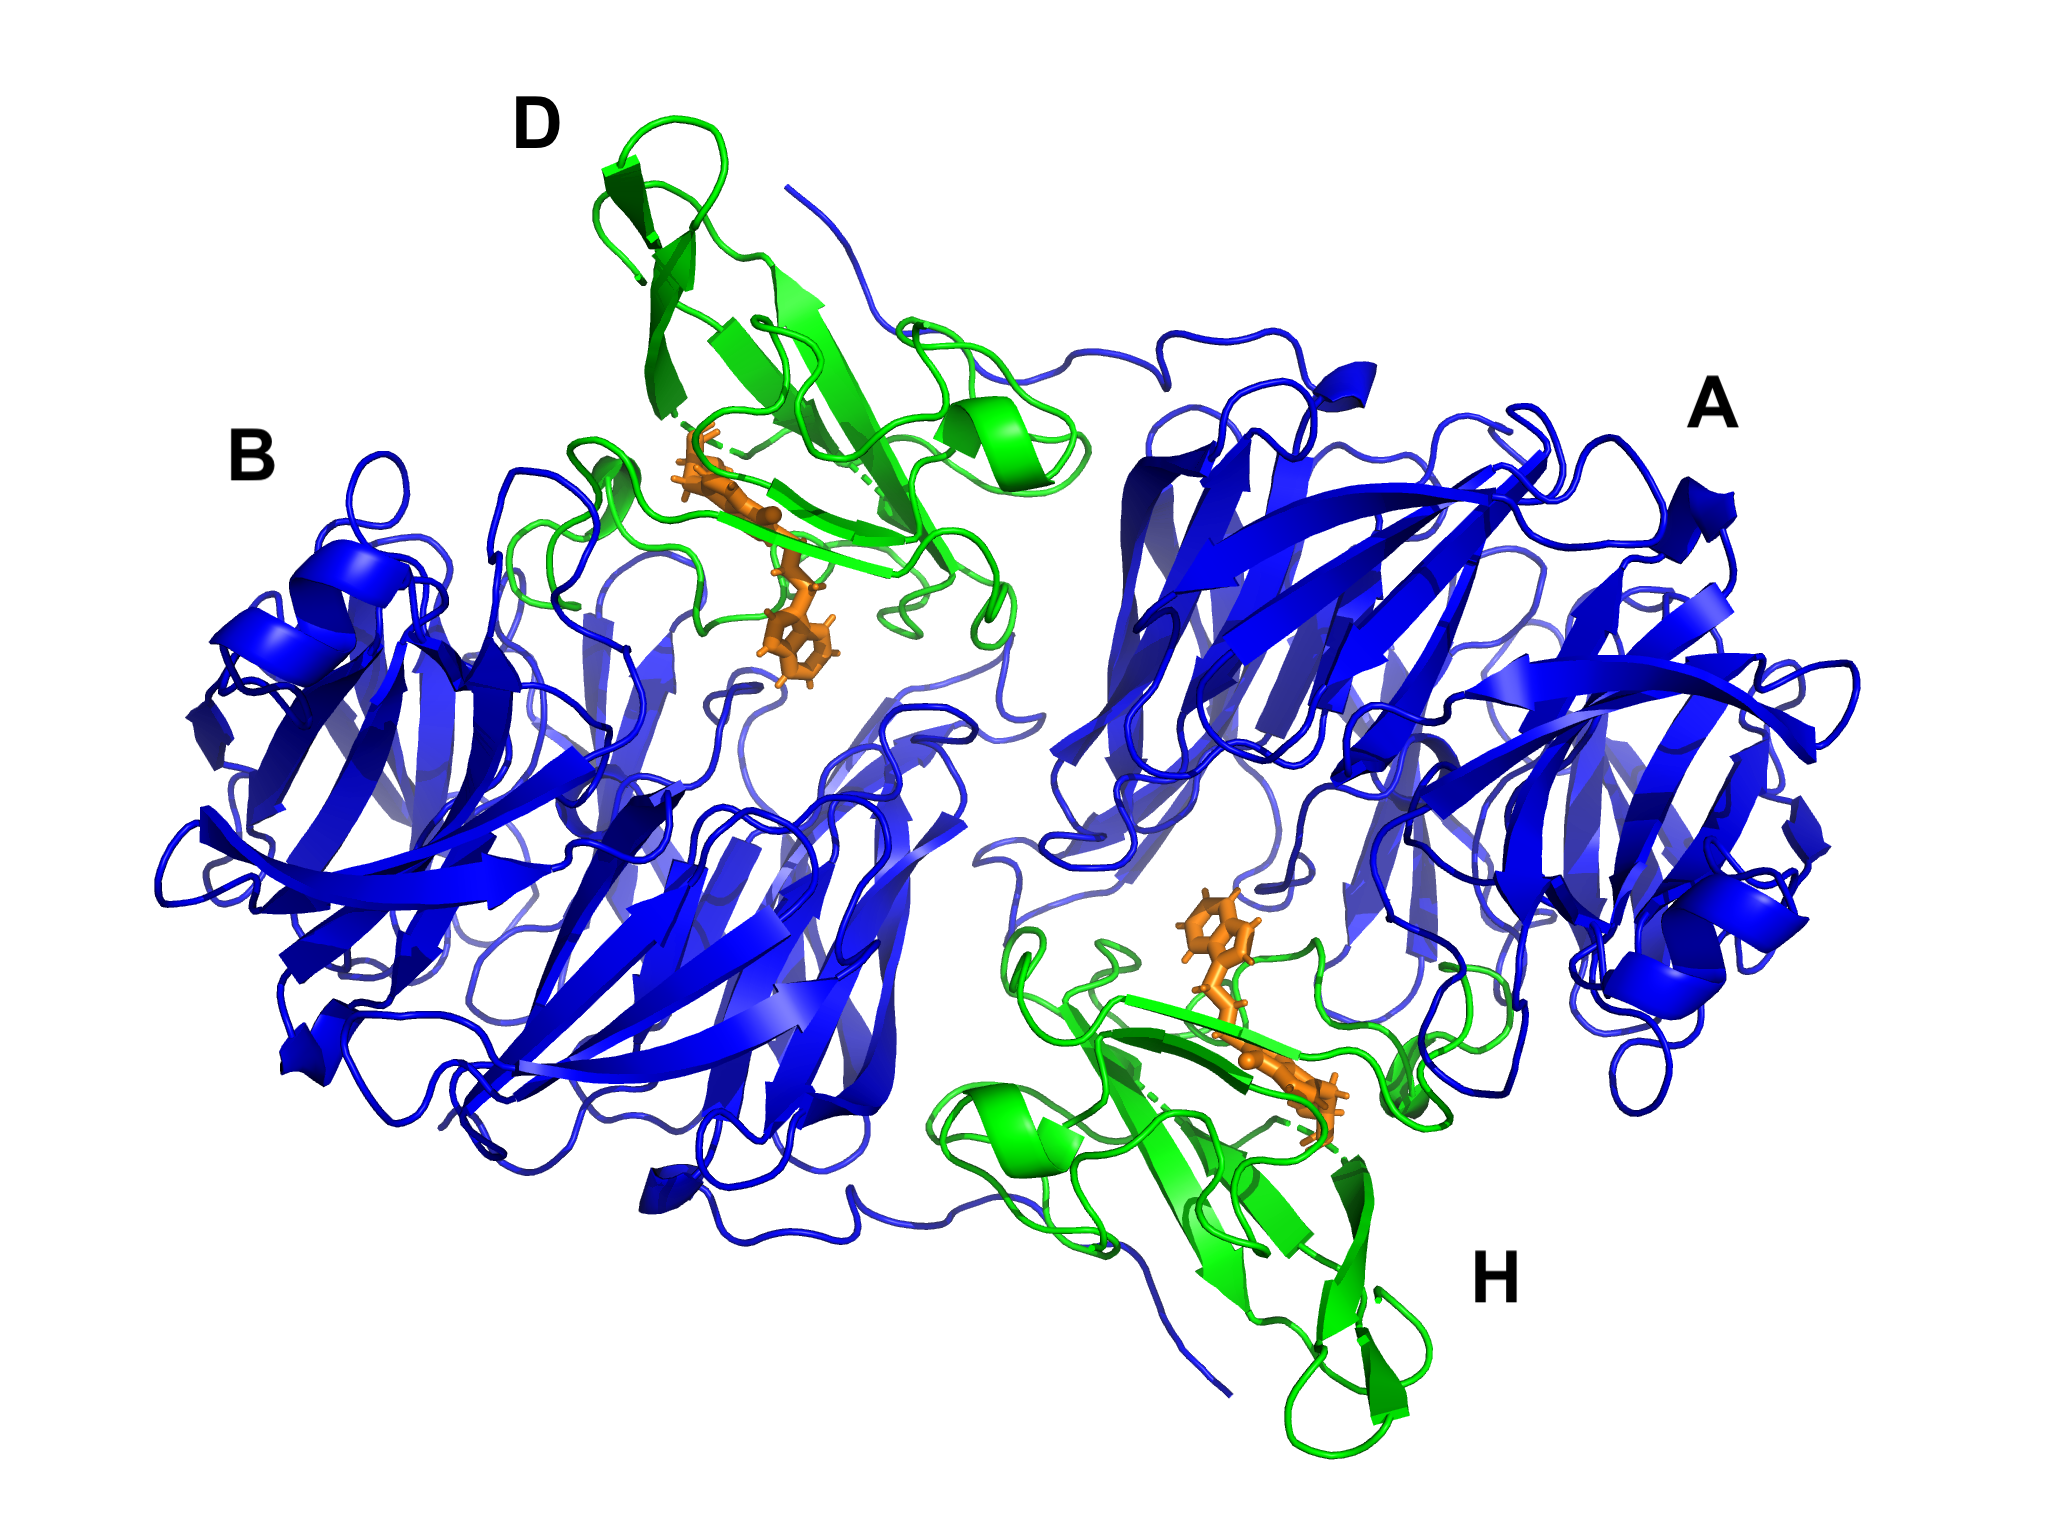
\includegraphics[width=0.8\textwidth]{chapters/aadh/figures/aadh_full_structure.png}
    \label{fig:aadh_full_structure}
\end{figure}

Aromatic amine dehydrogenase (AADH) was isolated from alcaligenses faecalis\cite{nozakiAromaticAmineDehydrogenase1987} a gram-negative soil bacterium\cite{govindarajAromaticAmineDehydrogenase1994a}. Amines are natural by-products of human activity and their degradation is an is an important part of the natural cycle which maintains their balance within organisms and the environment\cite{chistoserdovCloningSequencingMutagenesis2001}. AADH has an $\alpha_{2}\beta_{2}$ structure shown in figure \ref{fig:aadh_full_structure}. The larger $\alpha$ chains have a mass of $\simeq \SI{39}{\kilo\dalton}$ (shown in green and labelled A and B in the crystal structure) while the smaller $\beta$ chains (shown in blue, labelled D and H in the crystal structure) have a mass of $\simeq \SI{18}{\kilo\dalton}$. The D and H chains contain the TTQ prosthetic group that forms part of the active site (shown in orange, after reaction with tryptamine). 

\begin{figure}[p]
    \centering
    \mycaption[The proposed reaction mechanism of AADH]{\textsc{The proposed reaction mechanism of AADH}. This figure is adapted from figure 2 in\cite{masgrauAtomicDescriptionEnzyme2006}. The TTQ prosthetic group is shown in purple, the Asp128$\beta$ group in red and the tryptamine substrate in blue. The boxed step $4$ is the rate determining tunnelling step and step $7$ is the oxidation step. }
    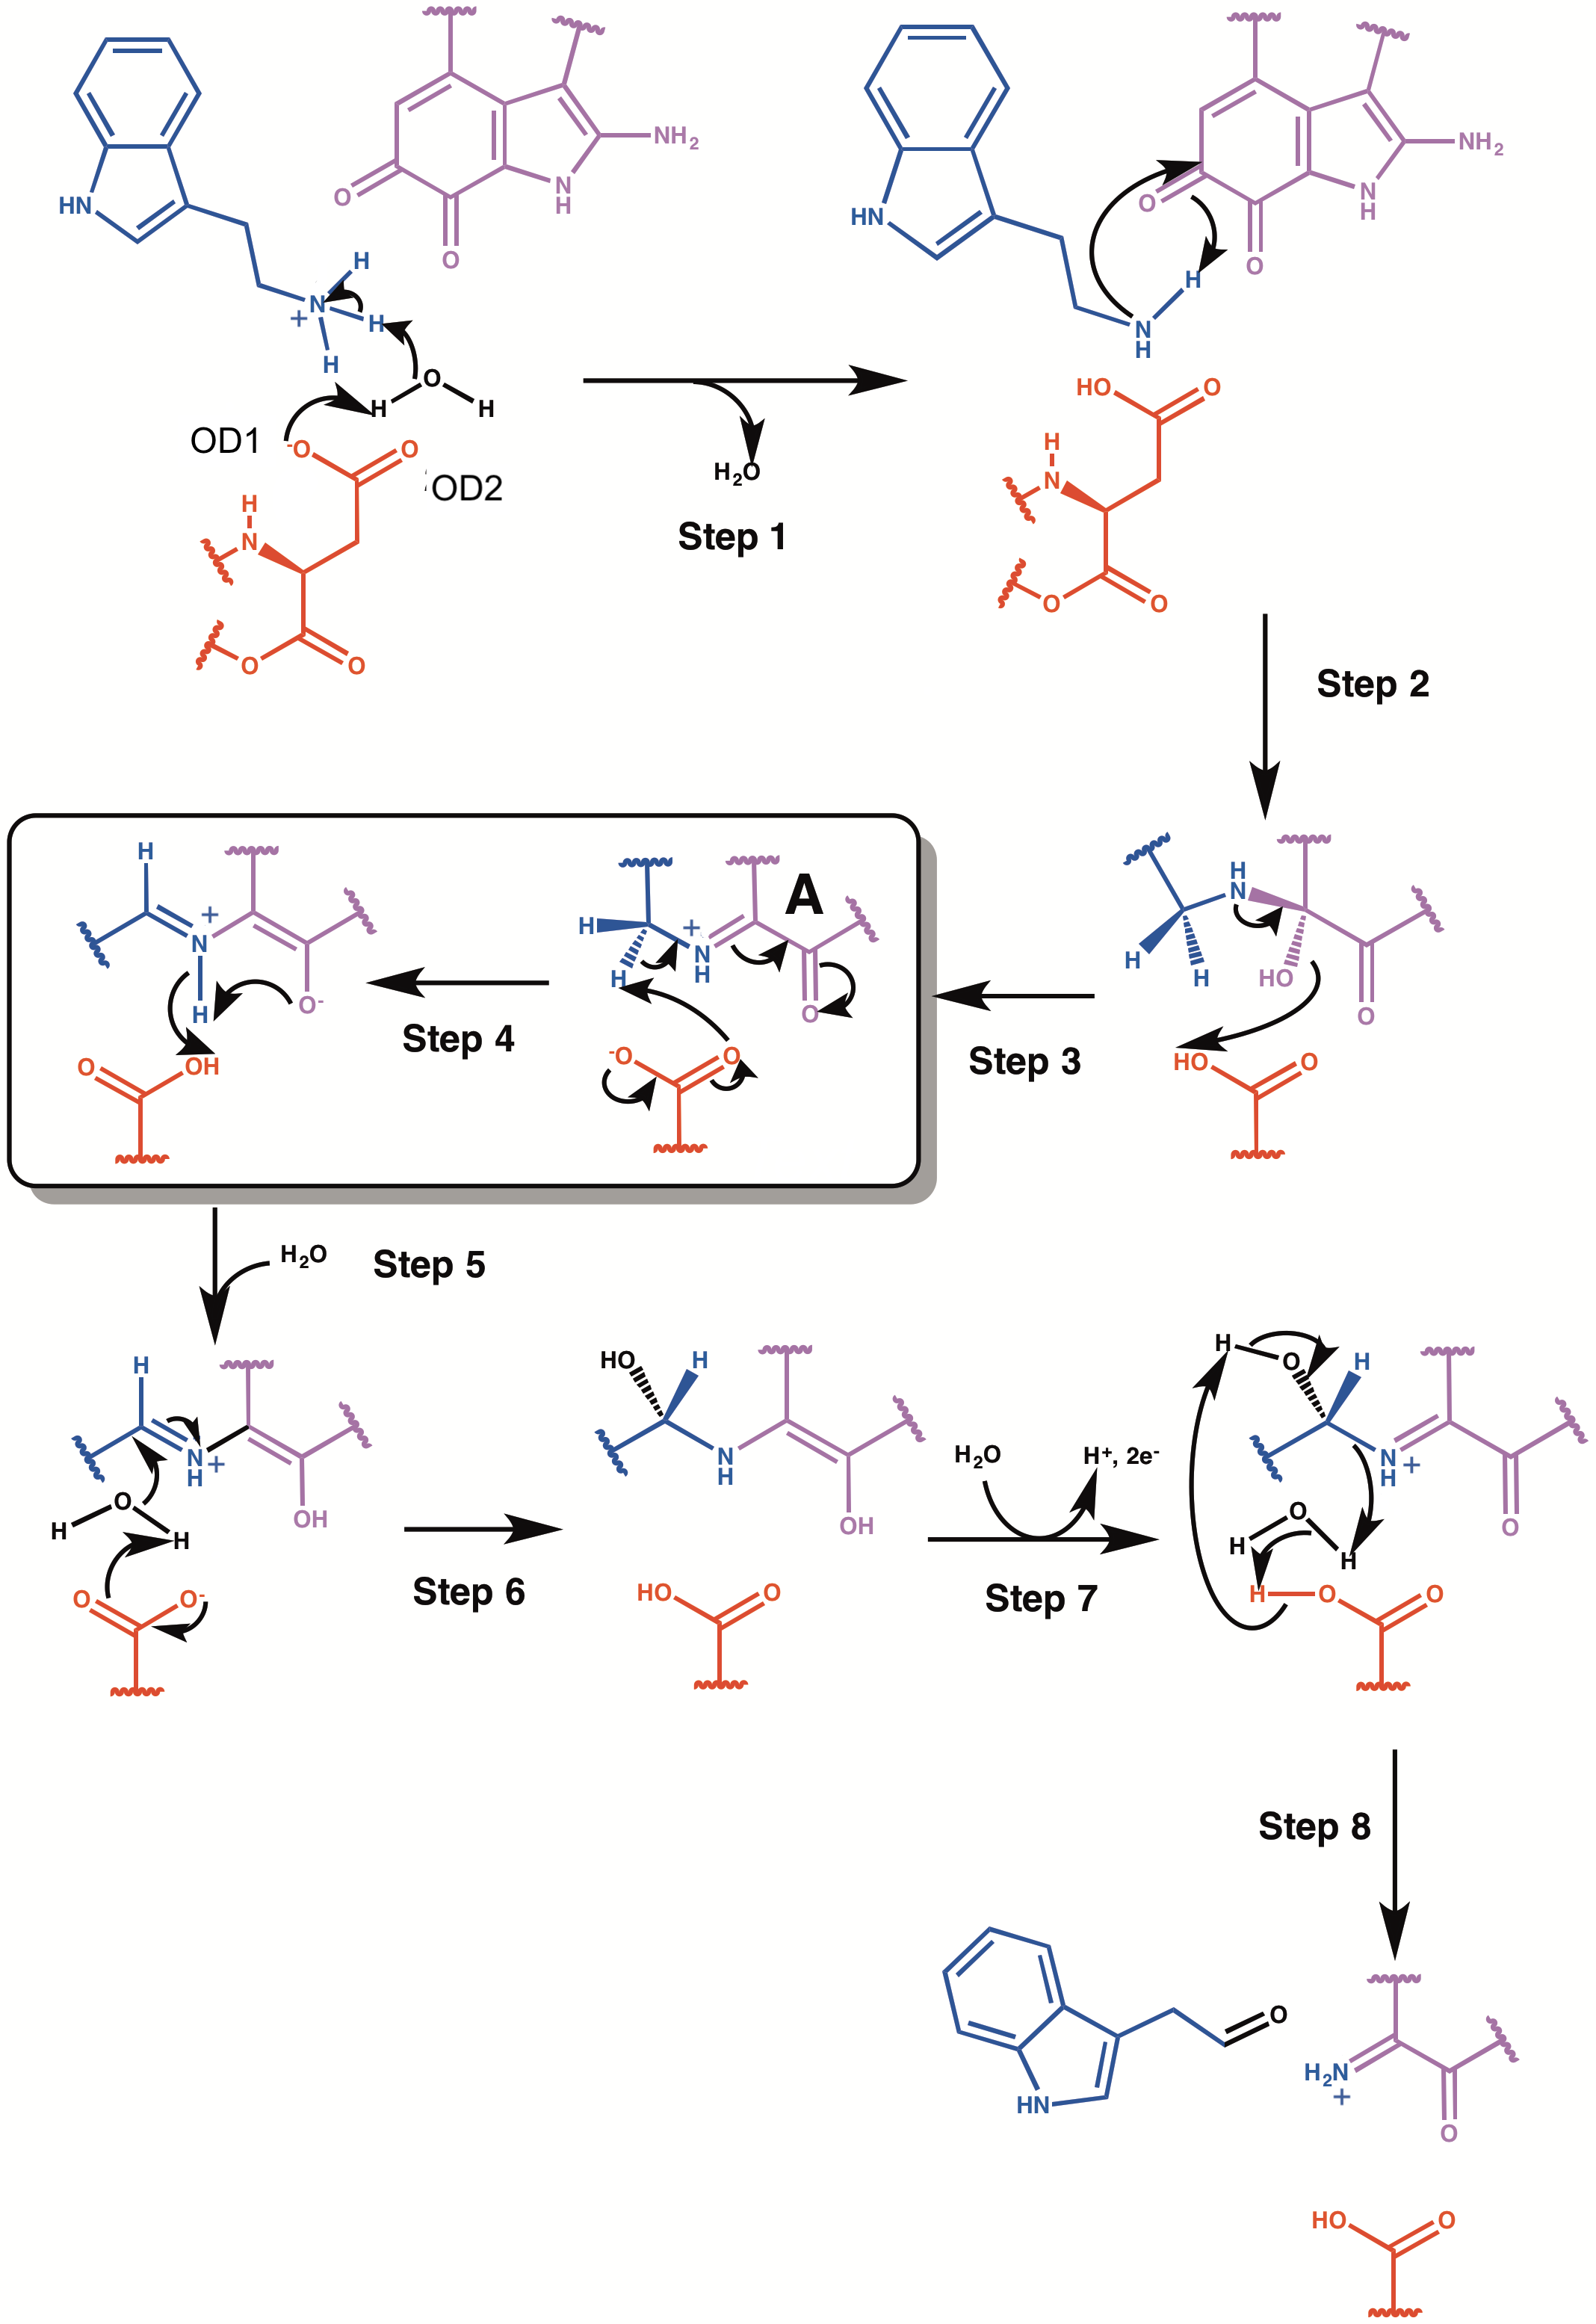
\includegraphics[ width=0.8\textwidth]{chapters/aadh/figures/aadh_mechanism.png}
    \label{fig:aadh_mechanism}
\end{figure}

The reaction mechanism of AADH was proposed in reference \cite{hyunMechanisticStudiesAromatic1995a} and more fully elucidated by a combination X-ray crystallography, experimental and QM/MM studies in references \cite{masgrauAtomicDescriptionEnzyme2006,masgrauTunnelingClassicalPaths2007, ranaghanInitioQMMM2017}, all using tryptamine as a substrate. 
The reaction mechanism is shown in figure \ref{fig:aadh_mechanism} which has been adapted from figure 2 of reference \cite{masgrauAtomicDescriptionEnzyme2006}. The following description is also taken from reference \cite{masgrauAtomicDescriptionEnzyme2006}. The TTQ prosthetic group, attached to the $\beta$ sub-unit, is shown in purple, the protonated tryptamine substrate is shown in blue and the Asp128 residue is shown in red.  The mechanism starts with the enzyme substrate complex of the protonated tryptamine situated next to the TTQ group and Asp128 residue. The tryptamine is deprotonated by oxygen 1 of the Asp128 residue via a bridging water molecule (step 1). The nitrogen atom on the tryptamine attacks one of the carbonyl groups of the TTQ residue to form a carbinol-amine intermediate (step 2) that then goes on to form the iminoquinone intermediate labelled `A' (step 3). Intermediate A was not observed directly but was inferred from the crystal structure of an analogous complex using phenylhydrazine in place of tryptamine. Step 4, shown boxed, is the rate determining step and involves the tunnelling of a proton from the tryptamine carbon atom adjacent to the nitrogen, to an oxygen atom of the Asp128 residue.  The proton is shown here accepted by oxygen 2 of the Asp128 carboxylate group, but in principle oxygen 1 could also serve as an acceptor. The oxyanion on the TTQ/substrate group (hereafter referred to as TTW) is then neutralized by protonation from Asp128 via the hydrogen atom on the protonated Schiff base (step 5). Water is introduced and in step 6 attacks the Schiff base to form a carbinolamine intermediate that is then oxidized in step 7.  The carbinolamine is then hydrolysed in step 8 and releases the aldehyde.  


The experimental free energy barrier for this reaction is approximately\footnote{No error estimate was given in reference \cite{masgrauAtomicDescriptionEnzyme2006}.} $ \SI{12.7}{\kilo\cal\per\mol}$ at $T=\SI{300}{\kelvin}$ with a primary kinetic isotope effect of $55 \pm 6$, independent of temperature\cite{masgrauAtomicDescriptionEnzyme2006} for $T =\SIrange[range-phrase=-]{278}{298}{\kelvin}$. The high KIE is indicative of the hydrogen tunneling through the reaction barrier \cite{masgrauAtomicDescriptionEnzyme2006,kohenEnzymeCatalysisClassical1998,antoniouInternalEnzymeMotions2001,antoniouLargeKineticIsotope1997,allemannQuantumTunnellingEnzymecatalysed2009}. The rate determining hydrogen abstraction can proceed to either OD1 or OD2 of the Asp128. These two atoms are distinguished by the hydrogen bonding network: OD2 is hydrogen bonded to Trp160, and OD1 to Thr172 as shown in figure \ref{fig:aadh_active_site}. In previous AADH simulation studies, \cite{masgrauAtomicDescriptionEnzyme2006,masgrauTunnelingClassicalPaths2007,ranaghanInitioQMMM2017}, the authors labelled OD1 as O2 and OD2 as O1, this convention is not adopted here as the accessible conformations allow OD1 and OD2 to hydrogen bond to both Trp160 and Thr172, so the force-field atoms names will be retained. 

The authors of reference \cite{ranaghanInitioQMMM2017} calculated the potential energy surface for pathways to both oxygen atoms using nudged elastic band with QM/MM using DH\&HLYP/6-311+G(d)/MM. Although not the aim of this study, they incorporated zero-point energy, tunneling and entropic contributions of previous studies\cite{masgrauAtomicDescriptionEnzyme2006,masgrauTunnelingClassicalPaths2007} to estimate the free energy barriers to OD1 and OD2 as $\SI{11.5}{\kilo\cal\per\mol}$ and $\SI{8.84}{\kilo\cal\per\mol}$ respectively, meaning both pathways are distinct but indistinguishable from the experimental free energy.  

AADH and the other known amine dehydrogenase, methylamine dehydrogenase (MADH) are of continued scientific interest because of their large kinetic isotope effect (KIE)\cite{hyunUnusuallyLargeIsotope1995a,basranImportanceBarrierShape2001a,basranEnzymaticHTransferRequires1999}, its anomalous time dependence\cite{glowackiProteinDynamicsEnzyme2012a, glowackiTakingOckhamRazor2012b} and the potential role of dynamics in explaining its catalytic function\cite{mcgeaghProteinDynamicsEnzyme2011,glowackiProteinDynamicsEnzyme2012a,glowackiTakingOckhamRazor2012b}. Both MADH and AADH contain the tryptophan tryptophylquinone (TTQ) prosthetic group\cite{govindarajAromaticAmineDehydrogenase1994a,McIntire817}, formed from two cross-linked tryptophyl residues.


Current theory on the role of protein dynamics in promoting tunneling \cite{kuznetsovProtonHydrogenAtom1999a,masgrau2004hydrogen} uses two types of protein dynamics to explain the rate constants and the temperature dependence of the KIE. `Active dynamics' which enhance the probability of tunneling occurring in a given conformation, and `passive dynamics' which re-arrange the enzyme to achieve such a suitable conformation. Active vibrations, on the sub-picosecond timescale, have been identified in AADH\cite{johannissenEnzymeAromaticAmine2008,johannissenProtonTunnelingAromatic2007} which act to promote the tunneling reaction.  However, the KIE in AADH is independent of temperature\cite{masgrauAtomicDescriptionEnzyme2006}, indicative of passive dynamics being the dominant factor in explaining the observed rate constant. Furthermore in \cite{glowackiProteinDynamicsEnzyme2012a,glowackiTakingOckhamRazor2012b} the authors showed that the kinetics and KIEs of a number of enzymes with large KIEs, including AADH, could be fitted to a simple extension of Transition State Theory (TST). This model posits two interconverting enzyme conformations each linked to a reaction coordinate with different reaction barriers. While this model can be made to  realistically fit experimental data, the conformers, their number and the exact values of the model parameters have not been fully validated. 

It is clear that an accurate and comprehensive description of the conformational dynamics of AADH would be useful in adding to the ongoing debate of enzyme dynamics and their role in catalysis. This chapter attempts to provide such a description utilising the techniques demonstrated in chapters \ref{chap:msm} and \ref{chap:hmm} for optimally building and coarse-graining a Markov state model, and is structured as follows: section \ref{sec:aadh_md} describes the creation of a molecular dynamics data set and compares it to existing computational studies of the reaction mechanism. Section \ref{sec:aadh_optimisation} uses the optimisation techniques from chapter \ref{chap:msm} to create an optimal discretization of the MD data set. This is then coarse-grained in section \ref{sec:aadh_hmm} using an hidden Markov model with the number of metastable states determined using the ICL as described in chapter \ref{chap:hmm}. A short summary and discussion of the implications of the final set of models is given in section \ref{sec:aadh_landscape} and section \ref{sec:aadh_conclusions} concludes and discusses  the limitations. 

\section{Molecular dynamics}\label{sec:aadh_md}

A PDB of AADH was prepared by Dr Kara Ranaghan as described in section \ref{sec:aadh_contributions} at the start of this chapter. The atom types in TTW were changed to be compatible with the CHARMM-36\cite{huangCHARMM36AllatomAdditive2013} force-field although the TTW parameters remained the same. The CHARMM package, version 42a2\cite{brooksCHARMMBiomolecularSimulation2009} was used to create a protein structure file (PSF). 

A solvation shell tracking the surface of the protein was created using the package Solvate (version 1.0)\cite{grubmullerSolvate} which was modified by the author of this thesis to take into account the CHARMM extended PSF format for large systems. The water shell was \SI{12.0}{\angstrom} thick, the maximum boundary curvature radius of the solvent surface was \SI{100}{\angstrom}, and \num{10} Gaussian functions were used to determine the solvent surface. This structure was further solvated to create a cubic simulation cell of size \SI{130}{\angstrom} using the package Visual Molecular Dynamics (VMD) (version 1.9.3)\cite{HUMP96} with a boundary parameter equal to \SI{1.2}{\angstrom}. The size of the box was chosen so that the minimum distance between the enzyme and the edge of the simulation cell was  \SI{14}{\angstrom}. The system was neutralized with VMD using sodium chloride to attain a concentration of \SI{0.15}{\molar}. 
The minimization, heating and equilibration steps were performed in CHARMM with the OpenMM\cite{OpenMMRapidDevelopment} plug-in using the CHARMM-36m\cite{huangCHARMM36AllatomAdditive2013} force-field. The electronic non-bonded forces in all steps were treated with partial mesh Ewald summation\cite{dardenParticleMeshEwald1993} with a cut-off of \SI{14}{\angstrom}, all other parameters were set to their default values. The SHAKE\cite{ryckaertNumericalIntegrationCartesian1977b} algorithm was used throughout to constrain the bonds to hydrogen atoms. The minimization proceeded by first restraining all heavy atoms  using a root mean square deviation (RMSD) restraint with a mass weighted force constant of \SI{5}{\kilo\cal\per\mol\per\square\angstrom} and then minimizing with \num{100} steps using the steepest descent algorithm and \num{3000} steps of adopted basis Newton-Raphson (ABNR) minimization. This was repeated three times, first limiting the  restraint to all the heavy protein atoms, then the heavy protein backbone atoms, and finally with no restraint. The final unrestrained minimization proceeded with \num{5000} instead of \num{3000} steps of ABNR minimization. 

The system was heated from \SIrange{10}{310}{\kelvin} in steps of \SI{25}{\kelvin}, with a harmonic restraint on the heavy protein backbone atoms with mass weighted force constant of \SI{5}{\kilo\cal\per\mol\per\square\angstrom}. At each heating step \SI{10}{\pico\second} of Langevin dynamics\cite{ermakComputerSimulationCharged1974,ermakEquilibriumElectrostaticEffects1974} in a constant volume, constant temperature ensemble were run with a time-step of \SI{2}{\femto\second} and collision frequency of $\gamma=\SI{5}{\per\pico\second}$. 

The system underwent equilibration in two stages: i) restrained equilibration and ii) unrestrained equilibration. In the restrained equilibration stage $11 \times \SI{20}{\pico\second}$ iterations of Langevin dynamics were run in an constant pressure, constant temperature ensemble (P=\SI{1}{\atm}, T=\SI{310}{\kelvin}), with a collision frequency $\gamma=\SI{1}{\per\pico\second}$, a Monte Carlo barostat with volume moves performed every \SI{50}{\femto\second}, and a time-step of \SI{2}{\femto\second}. On the first iteration the backbone atoms had a harmonic restraint with a mass weighted force constant of  \SI{10}{\kilo\cal\per\mol\per\square\angstrom}. On each subsequent iteration the force constant was reduced by \SI{1}{\kilo\cal\per\mol\per\square\angstrom} until the last iteration had no harmonic restraint. The unrestrained equilibration consisted of \SI{200}{\pico\second} of equilibration run under the same conditions as before but with no restraints. 

The simulation system was transferred from CHARMM to AMBER (version 16)\cite{caseAMBER} to make use of the improved user interface and post-simulation analysis tools. A single  \SI{100}{\nano\second} trajectory was produced in a constant volume, constant temperature (T=\SI{310}{\kelvin}) ensemble, using Langevin dynamics with a collision frequency of $\gamma=\SI{5}{\per\pico\second}$, and a time step of \SI{2}{\femto\second}. The non-bonded cut-off distance was reduced to \SI{12}{\angstrom} and SHAKE\cite{ryckaertNumericalIntegrationCartesian1977b} was used to constrain the hydrogen atoms. Coordinates and velocities were written to disk every \SI{100}{\pico\second}.  

The coordinates and velocities at every \SIlist[list-final-separator = { ... }]{1; 2; 100}{\nano\second} were used to seed $100 \times \SI{100}{\nano\second}$ new trajectories, run under the same conditions. These \num{100} trajectories constituted the AADH data set. 

\subsection{Validation}\label{sec:aadh_validation}

\begin{figure}
    \centering
    \mycaption[Structural similarity of seed trajectory]{\textsc{Structural similarity of seed trajectory}. A \SI{100}{\nano\second} trajectory, with coordinates saved every \SI{1}{\nano\second} was used to seed \num{100} production trajectories.  Panel (a) shows the $\alpha$-carbon RMSD of the seed trajectory relative to the crystal structure, (b) shows the distribution of all pairwise $\alpha$-Carbon RMSD within the seed trajectory. }
    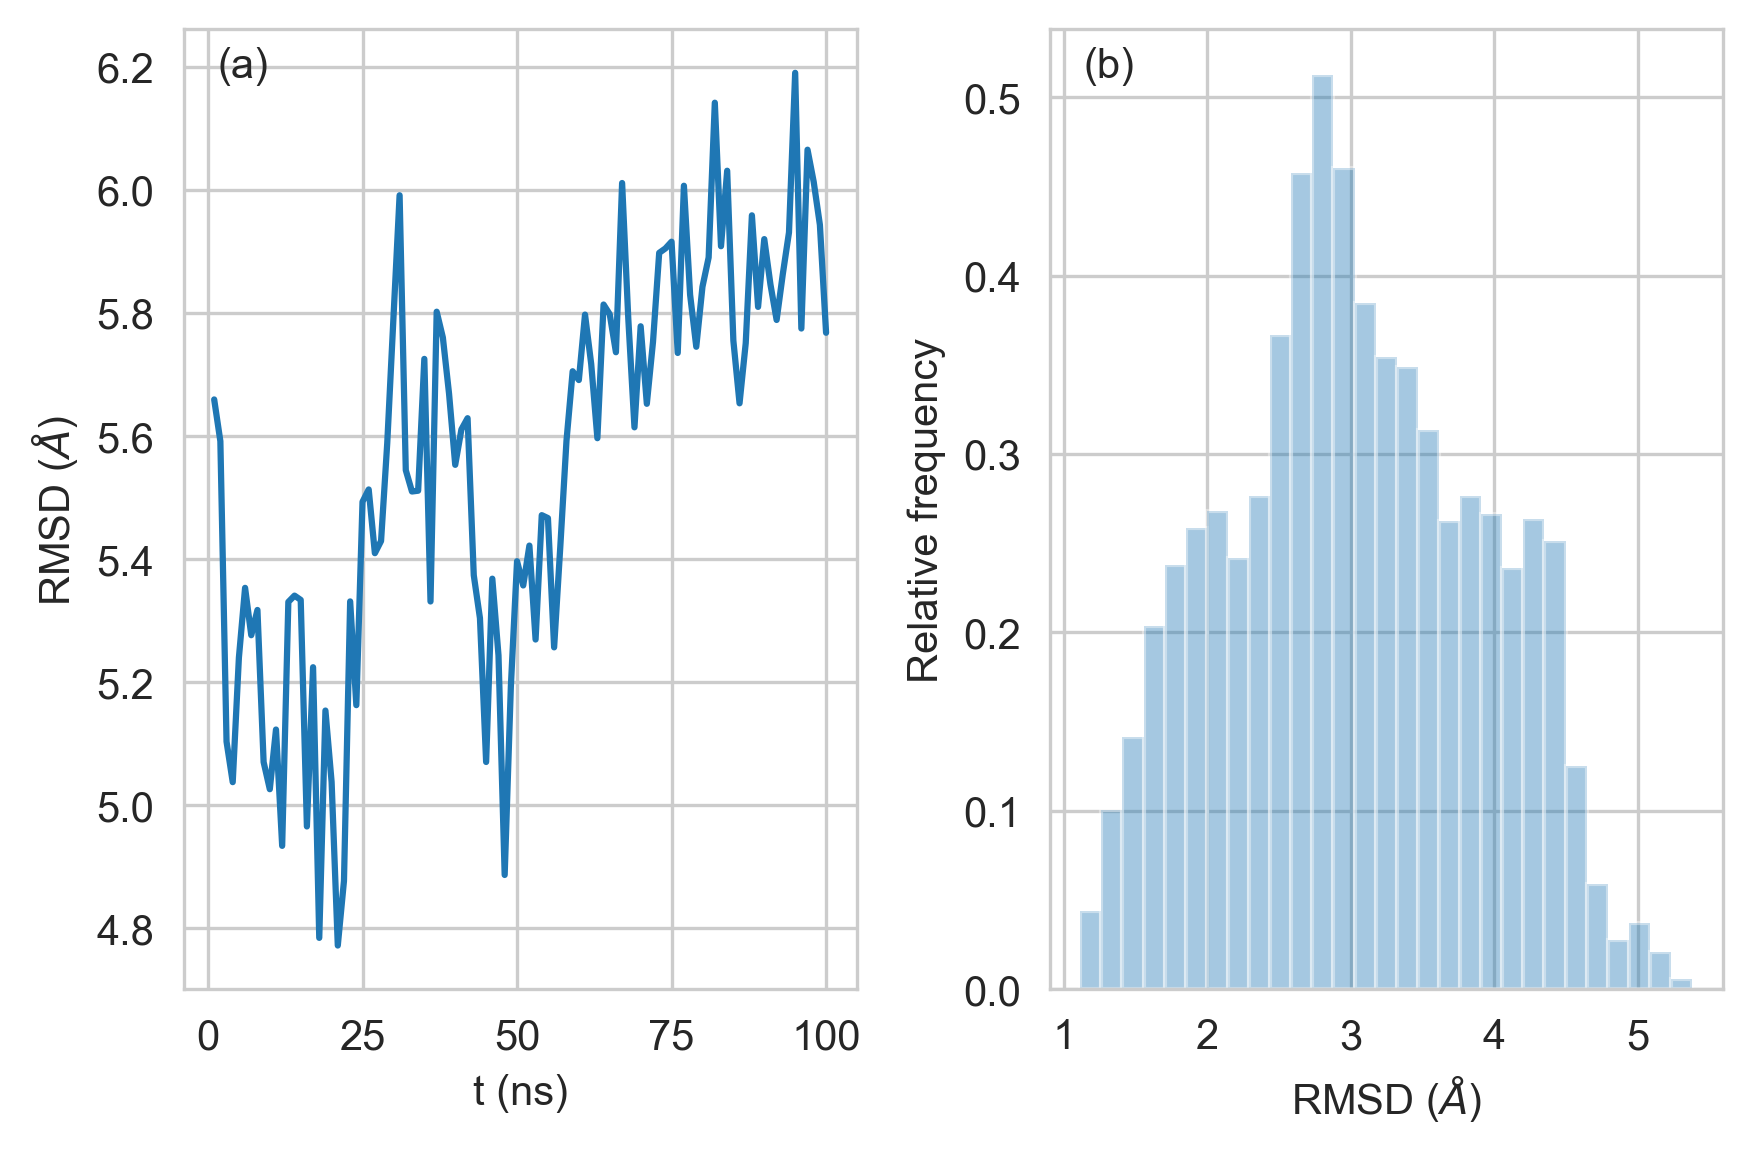
\includegraphics[width=0.8\textwidth]{chapters/aadh/figures/rmsd_seed_trajectory.png}
    \label{fig:rmsd_seed_traj}
\end{figure}
\begin{figure}
    \centering
    \mycaption[alpha-carbon deviation of residues from the seed trajectory]{\textsc{$\alpha$-carbon deviation of residues for seed trajectory}. Each panel depicts a separate chain of the structure from a snapshot of the seed trajectory at \SI{95}{\nano\second}. The RMSD is \SI{6.2}{\angstrom}, the highest value reached, see figure \ref{fig:rmsd_seed_traj} panel (a). In chains D and H the six residues of the active site are shown in orange and residues \numrange[range-phrase=-]{92}{108} are shown in green. The conformational change of loop \numrange[range-phrase=-]{92}{108} is shown in figure \ref{fig:chain_d_loop}}
    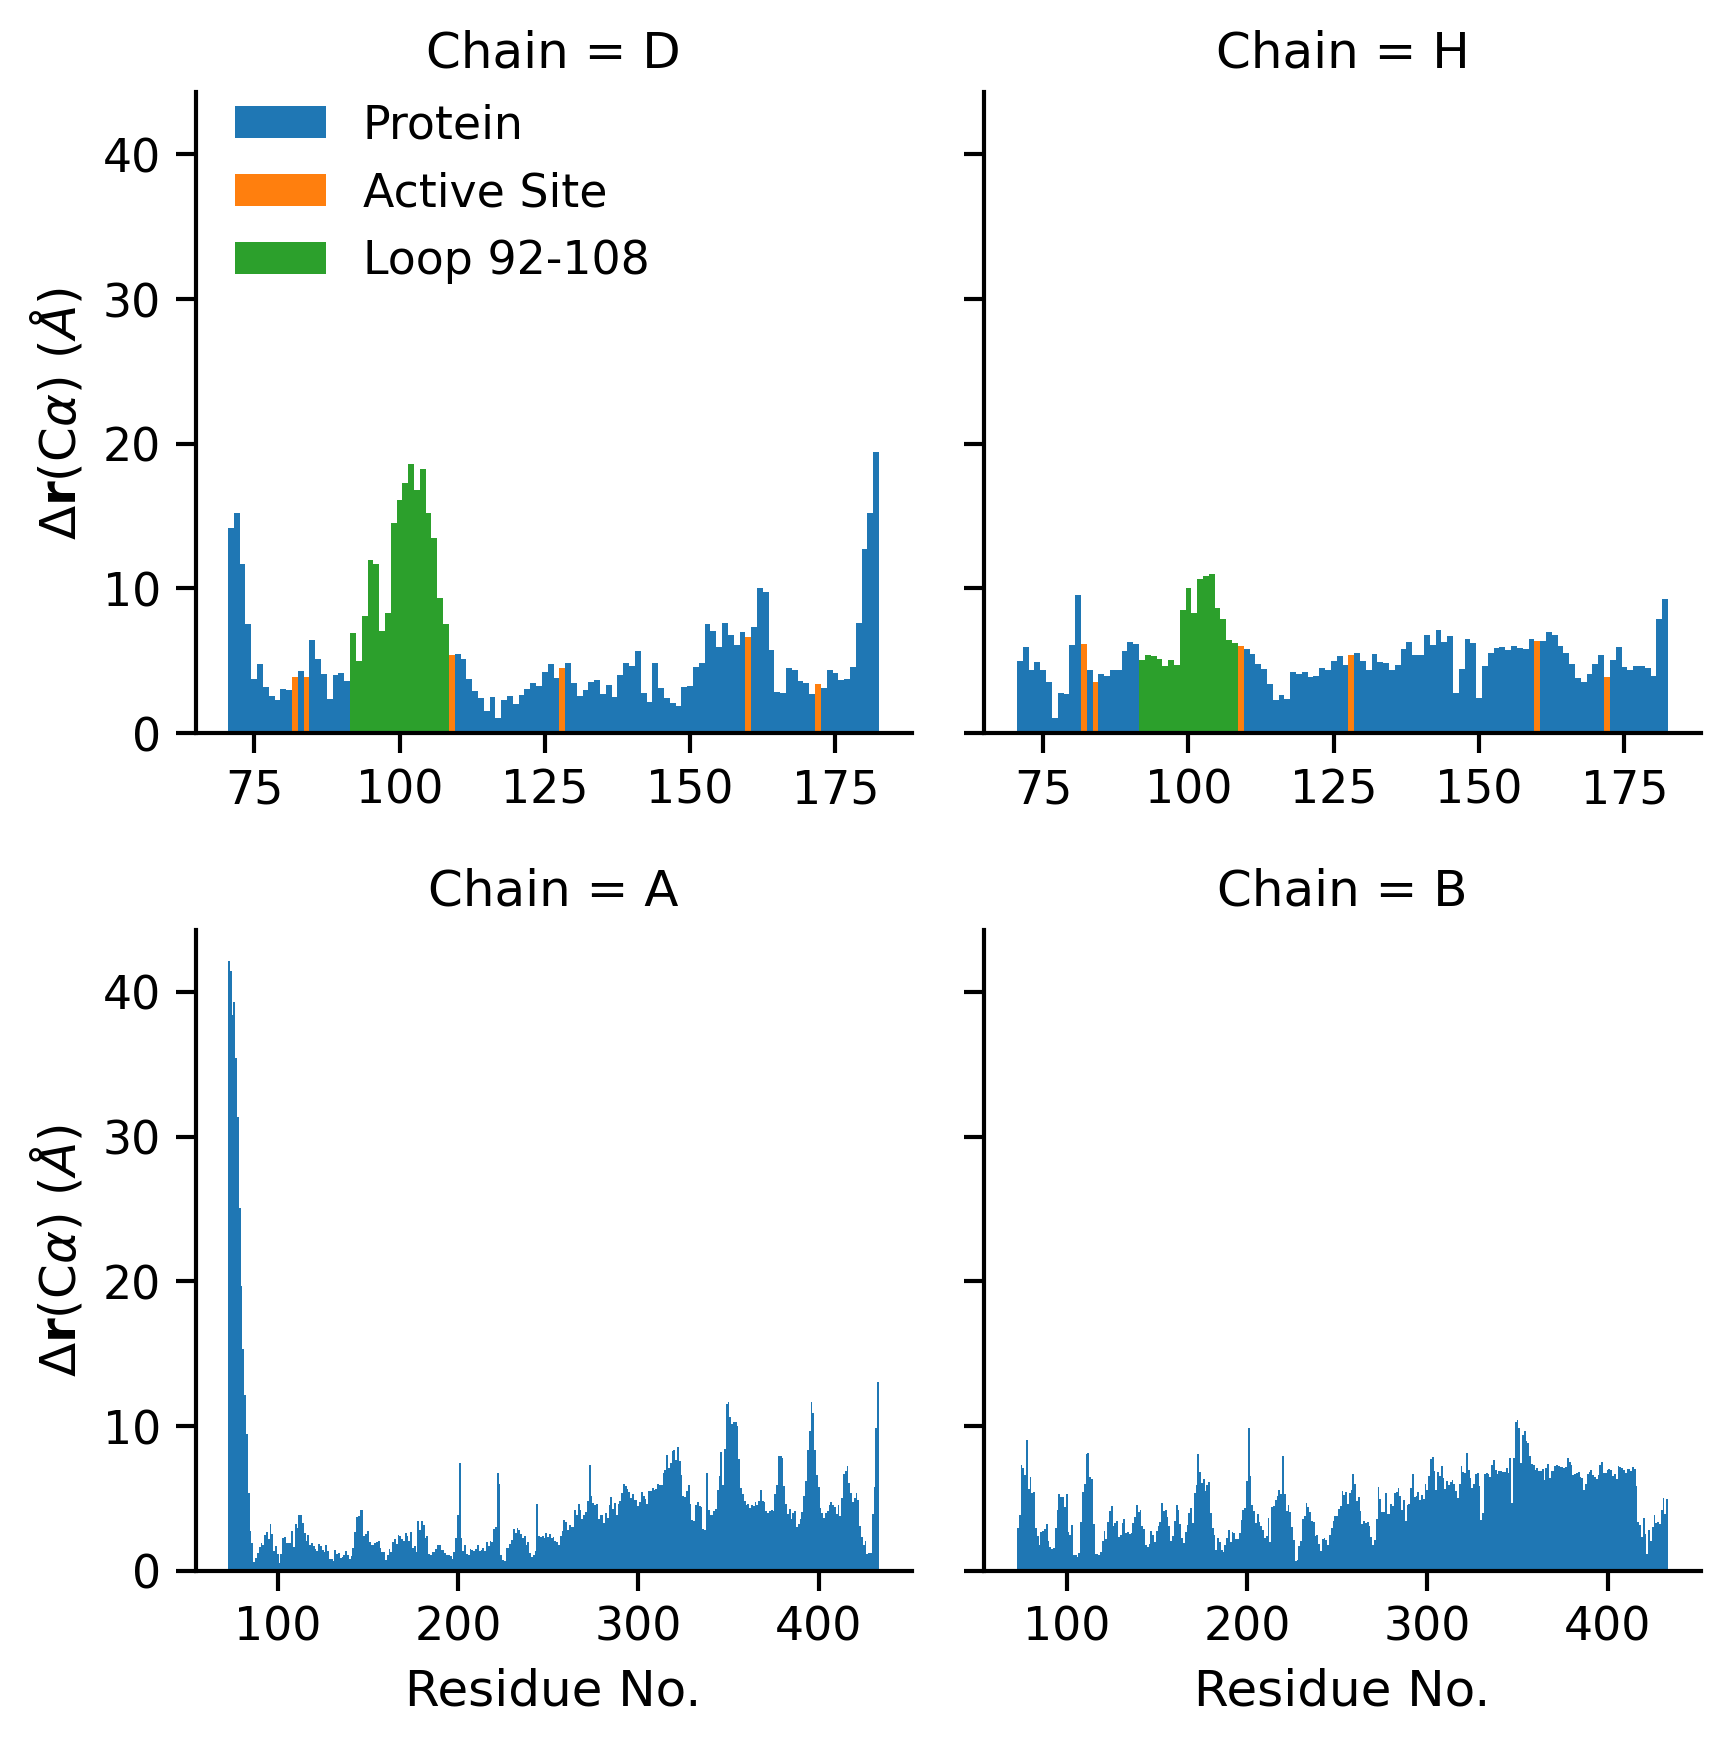
\includegraphics[width=0.8\textwidth]{chapters/aadh/figures/rmsd_by_res.png}
    \label{fig:aadh_rmsd_byres}
\end{figure}

An error was found in the preparation of the initial structure \emph{after} completion of the simulations. The disulphide bridge between Cys81 and Cys113 on the H chain (but not on the D chain) had not been created, instead the two thiol groups were left unoxidized. This will be discussed in full below. 

 The structural similarity between the initial frame of the each of the 100 production trajectories is shown in figure \ref{fig:rmsd_seed_traj}. Panel (a) shows the $\alpha$-carbon RMSD, relative to the crystal structure which shows a persistent, large deviation from the crystal structure and serial correlation between initial frames for $t>\SI{60}{\nano\second}$.  Panel (b) shows the distribution of $\alpha$-Carbon RMSD values between each pair of initial frames (i.e., there are $\sfrac{1}{2}\cdot 100\cdot 99 = 4950$ values in the histogram). This demonstrates a range of differences between the initial conformations: \SI{50}{\percent} of the initial structures have an RMSD of \SI{3.0}{\angstrom} or larger.  
 
The large absolute values of the RMSD are due to the residues at the tails of chains D and A, as well as residues \numrange[range-phrase=-]{92}{108} in chain D. This is shown in figure \ref{fig:aadh_rmsd_byres} which plots the $\alpha$-carbon deviation from the crystal structure of the seed trajectory at \SI{95}{\nano\second}. This frame was chosen as it had the highest RMSD (\SI{6.2}{\angstrom}) of the seed trajectory, shown in panel (a) of figure \ref{fig:aadh_rmsd_byres}. The $10$ residues with deviation of $>\SI{10}{\angstrom}$ at the N-terminus of chain A, clearly show a large contribution to the RMSD. Without these values the RMSD is reduced to \SI{5.3}{\angstrom}. Removing the six residues with a deviation $> \SI{10}{\angstrom}$  at the N- and C-terminus of chain D reduces the RMSD further to \SI{5.2}{\angstrom}. The loop residues \numrange[range-phrase=-]{92}{108} in chain D (and to a lesser extent chain H) show a large deviation due to a significant conformational change, shown in figure \ref{fig:chain_d_loop}. Without these loop residues the RMSD is reduced further to \SI{4.9}{\angstrom}. 

Each trajectory was checked for structural stability over the course of the simulations by calculating the RMSD of the $\alpha$-carbons atoms relative to the crystal structure, shown in figure \ref{fig:rmsd_ca}. The majority of the trajectories showed no increasing RMSD, indicative of potential change in secondary structure or major conformation change. \SI{95}{\percent} of the frames remained within \SIrange{4.5}{6.4}{\angstrom} of the crystal structure. However, seven of the trajectories (24, 27, 30, 42, 78, 87 and 97) had an RMSD trajectory which increased over time, leaving the upper \SI{95}{\percent} bound by at least the final frame, shown in figure \ref{fig:rmsd_ca}. The source of the increase in RMSD was not due to changing secondary structure (figure \ref{fig:dssp_trajs_sens}) but rather due to the high fluctuations in the tail residues, see figure xxx. 


\begin{figure}
    \centering
    \mycaption[The crystal structure of the active site of AADH]{\textsc{The crystal structure of the active site of AADH}. This definition is taken from reference \cite{ranaghanInitioQMMM2017} and consists of the following residues: Ala82, Asp84, TTW109, Asp128, Trp160 and Thr172. The yellow dashed lines show the important stabilizing hydrogen bonds as well as the H---O distances involved in the rate determining step.  The reactive hydrogen atoms are labelled HI-2 and HI-3. The acceptor oxygen atoms are labelled OD2 and OD1 which correspond to O1 and O2 in reference \cite{masgrauAtomicDescriptionEnzyme2006} respectively. All other hydrogen atoms are hidden. Backbone carbonyl bonds may appear as single bonds due to the camera angle.}
    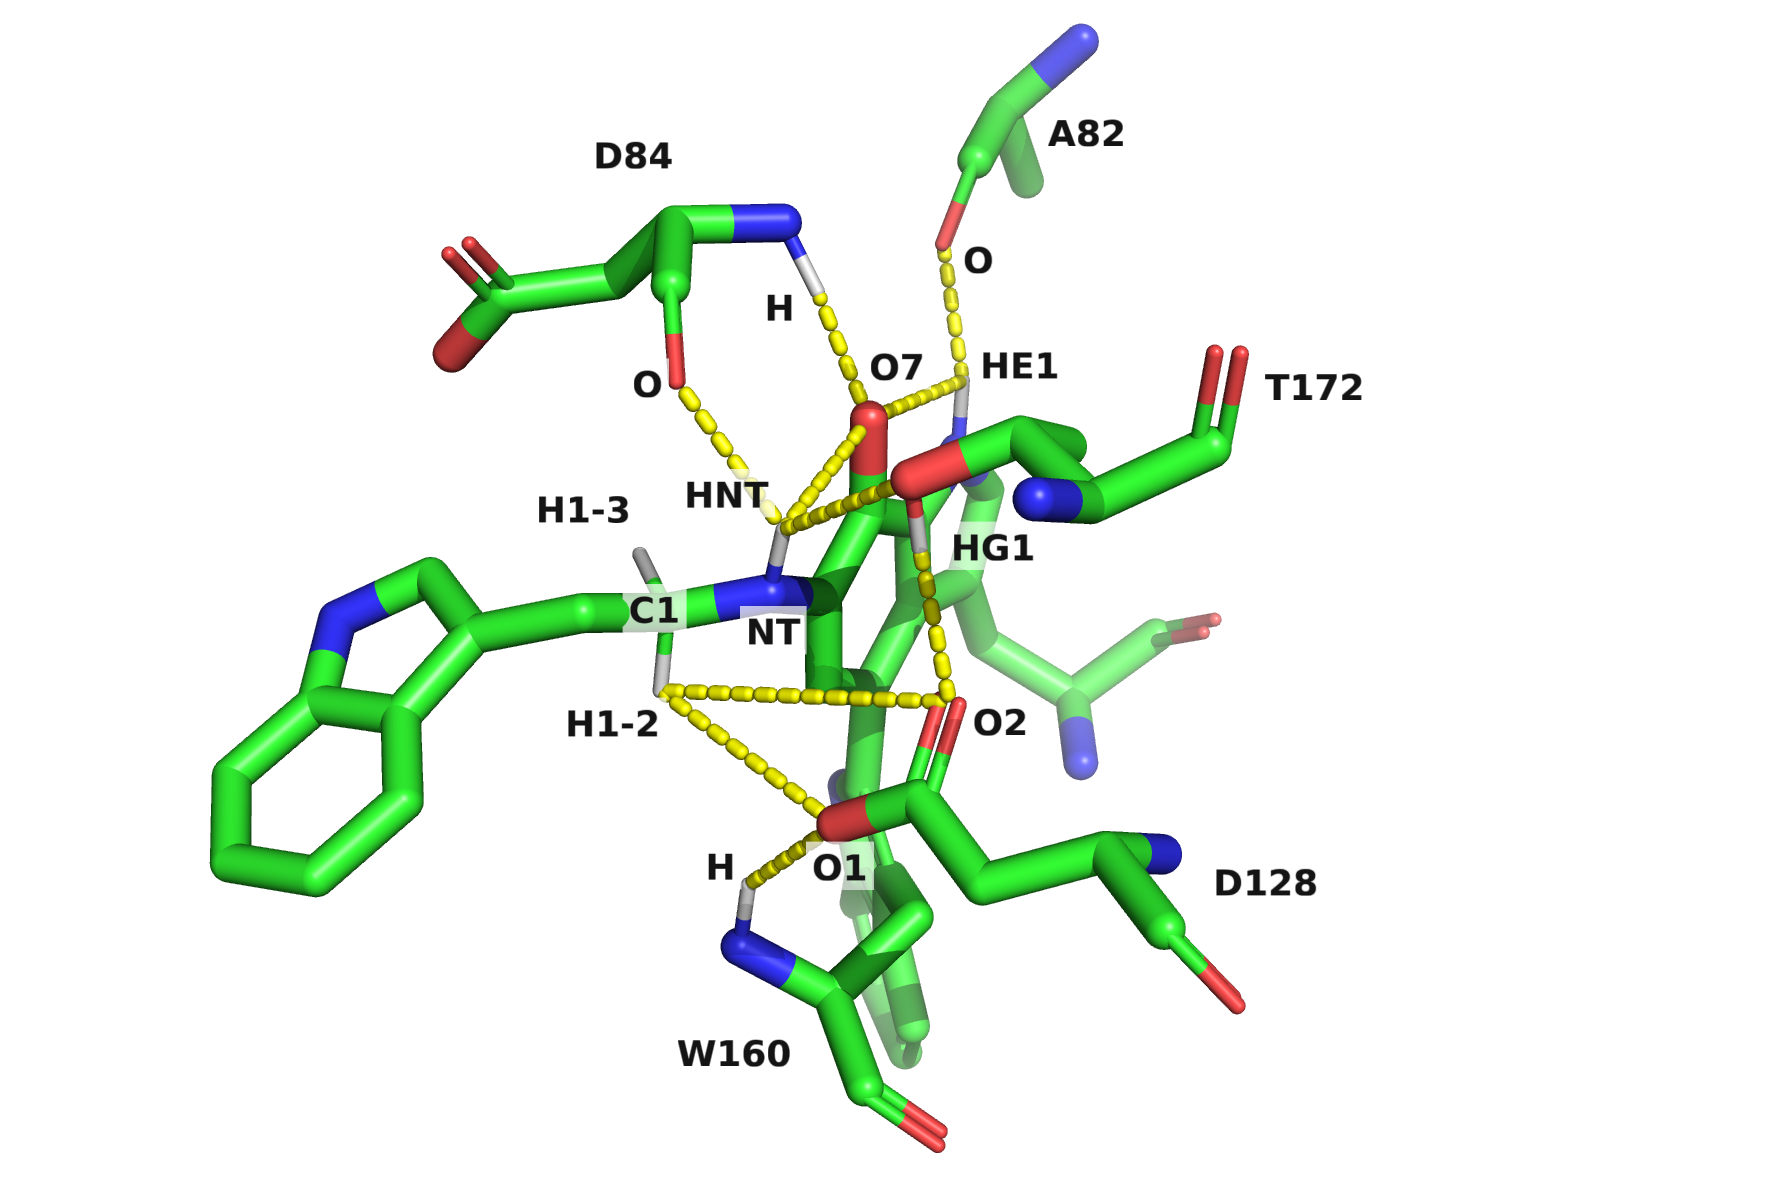
\includegraphics[width=0.8\textwidth]{chapters/aadh/figures/aadh_active_site.png}
    \label{fig:aadh_active_site}
\end{figure}

\begin{figure}
    \centering
    \mycaption[Comparison of the active site in chains D and H]{\textsc{Comparison of the active site in chains D and H}. The distribution of heavy atom RMSD, relative to the crystal structure of the active sites in chain D (blue) and H (orange). }
    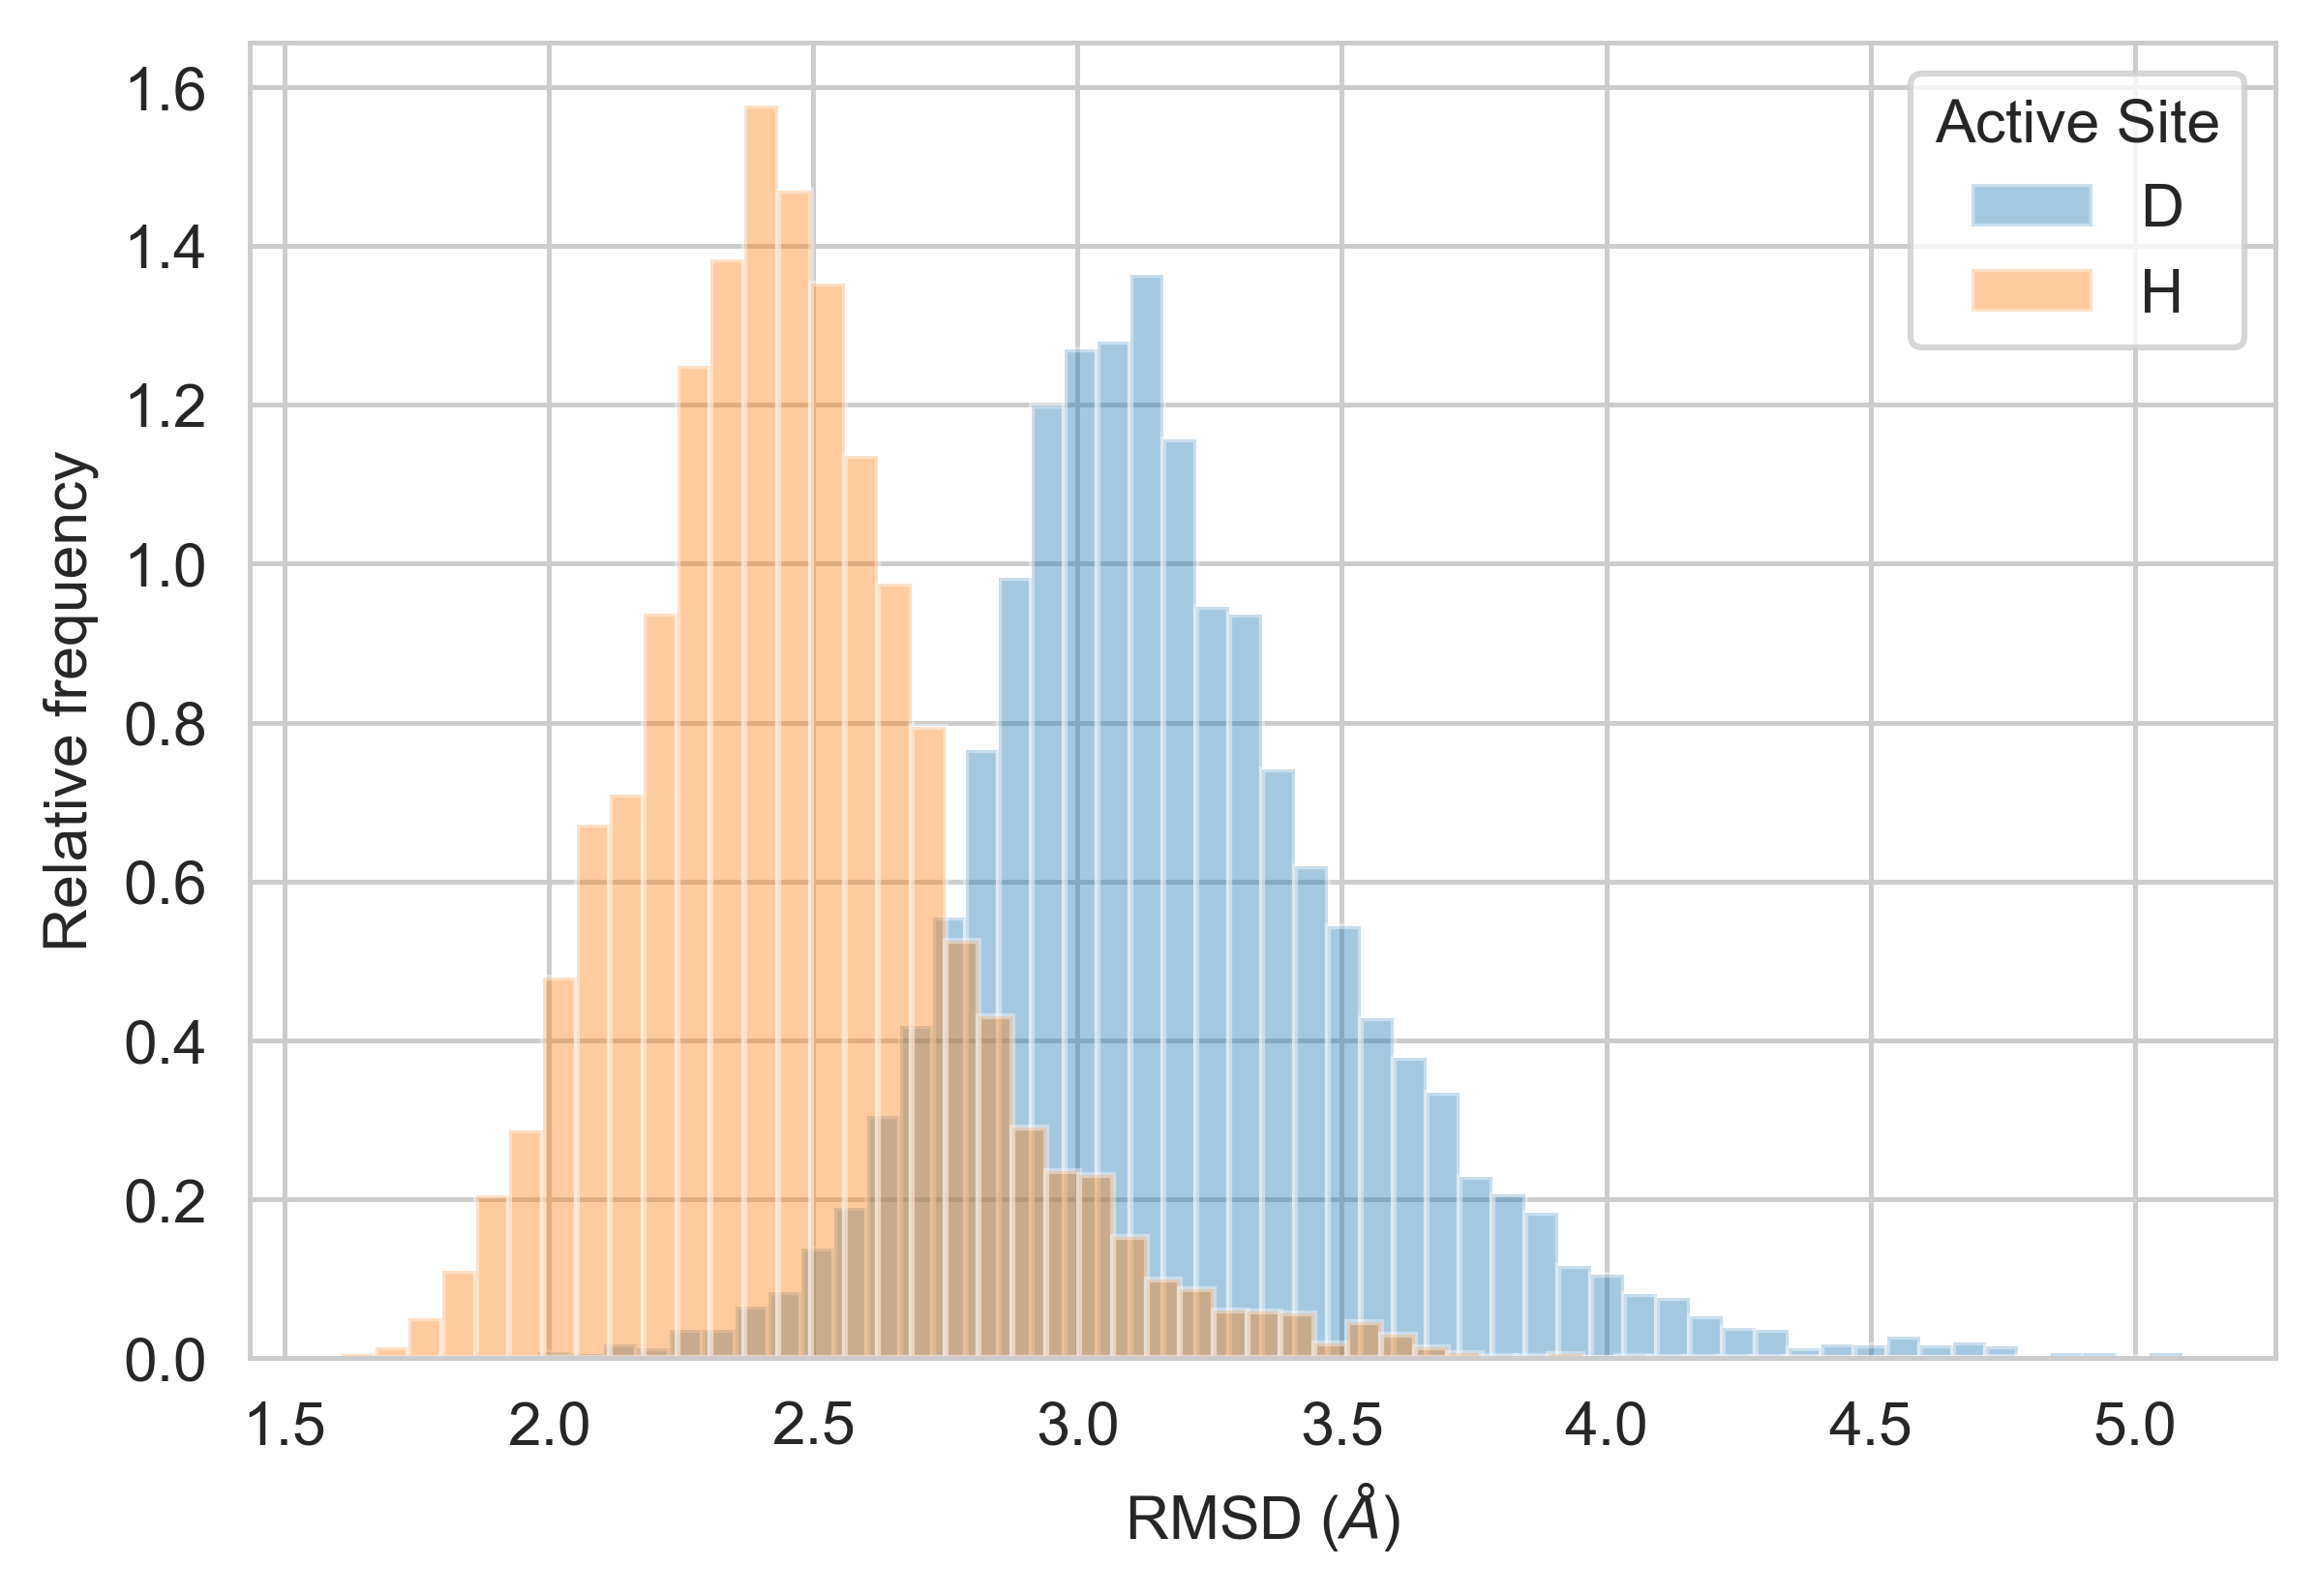
\includegraphics{chapters/aadh/figures/rmsd_dististribution.png}
    \label{fig:as_rmsd_dist}
\end{figure}

The active site of the enzyme was defined in the same way as references  \cite{ranaghanInitioQMMM2017, masgrauAtomicDescriptionEnzyme2006, masgrauTunnelingClassicalPaths2007} in chains D and H: Ala82, Asp84, TTW109, Asp128, Trp160 and Thr172. The TTW residue is the TTQ prosthetic group after reaction with the tryptamine substrate to form the Schiff base intermediate. Hereafter any reference to TTQ will refer to the portion of TTW coming from TTQ originally and not the unreacted prosthetic group. The crystal structure of the active site is shown in figure \ref{fig:aadh_active_site}. 

The structures of the two active sites were also compared to the crystal structure. The distribution of the heavy atom RMSD, relative to the crystal structure, is shown in figure \ref{fig:as_rmsd_dist}. This shows that the H active site is more structurally similar to the crystal structure than the D active site. This could be associated with the difference in the conformations of the loop residues \num{92}{108} between chain D and H in figure \ref{fig:aadh_rmsd_byres} and with the missing disulphide bond in chain H. However, this link has not been investigated. 

\begin{figure}
    \centering
    \mycaption[Distribution of important bond distances in the active site]{\textsc{Distribution of important bond distances in the active site}. Panels (a) - (d) show the four combinations of acceptor ion (O1, O2) - proton (H1-2, H1-3) distances; panels (e) and (f) are the two donor (C1) acceptor (O1, O2) distances; the remaining panels are the hydrogen bonds in the active site.}
    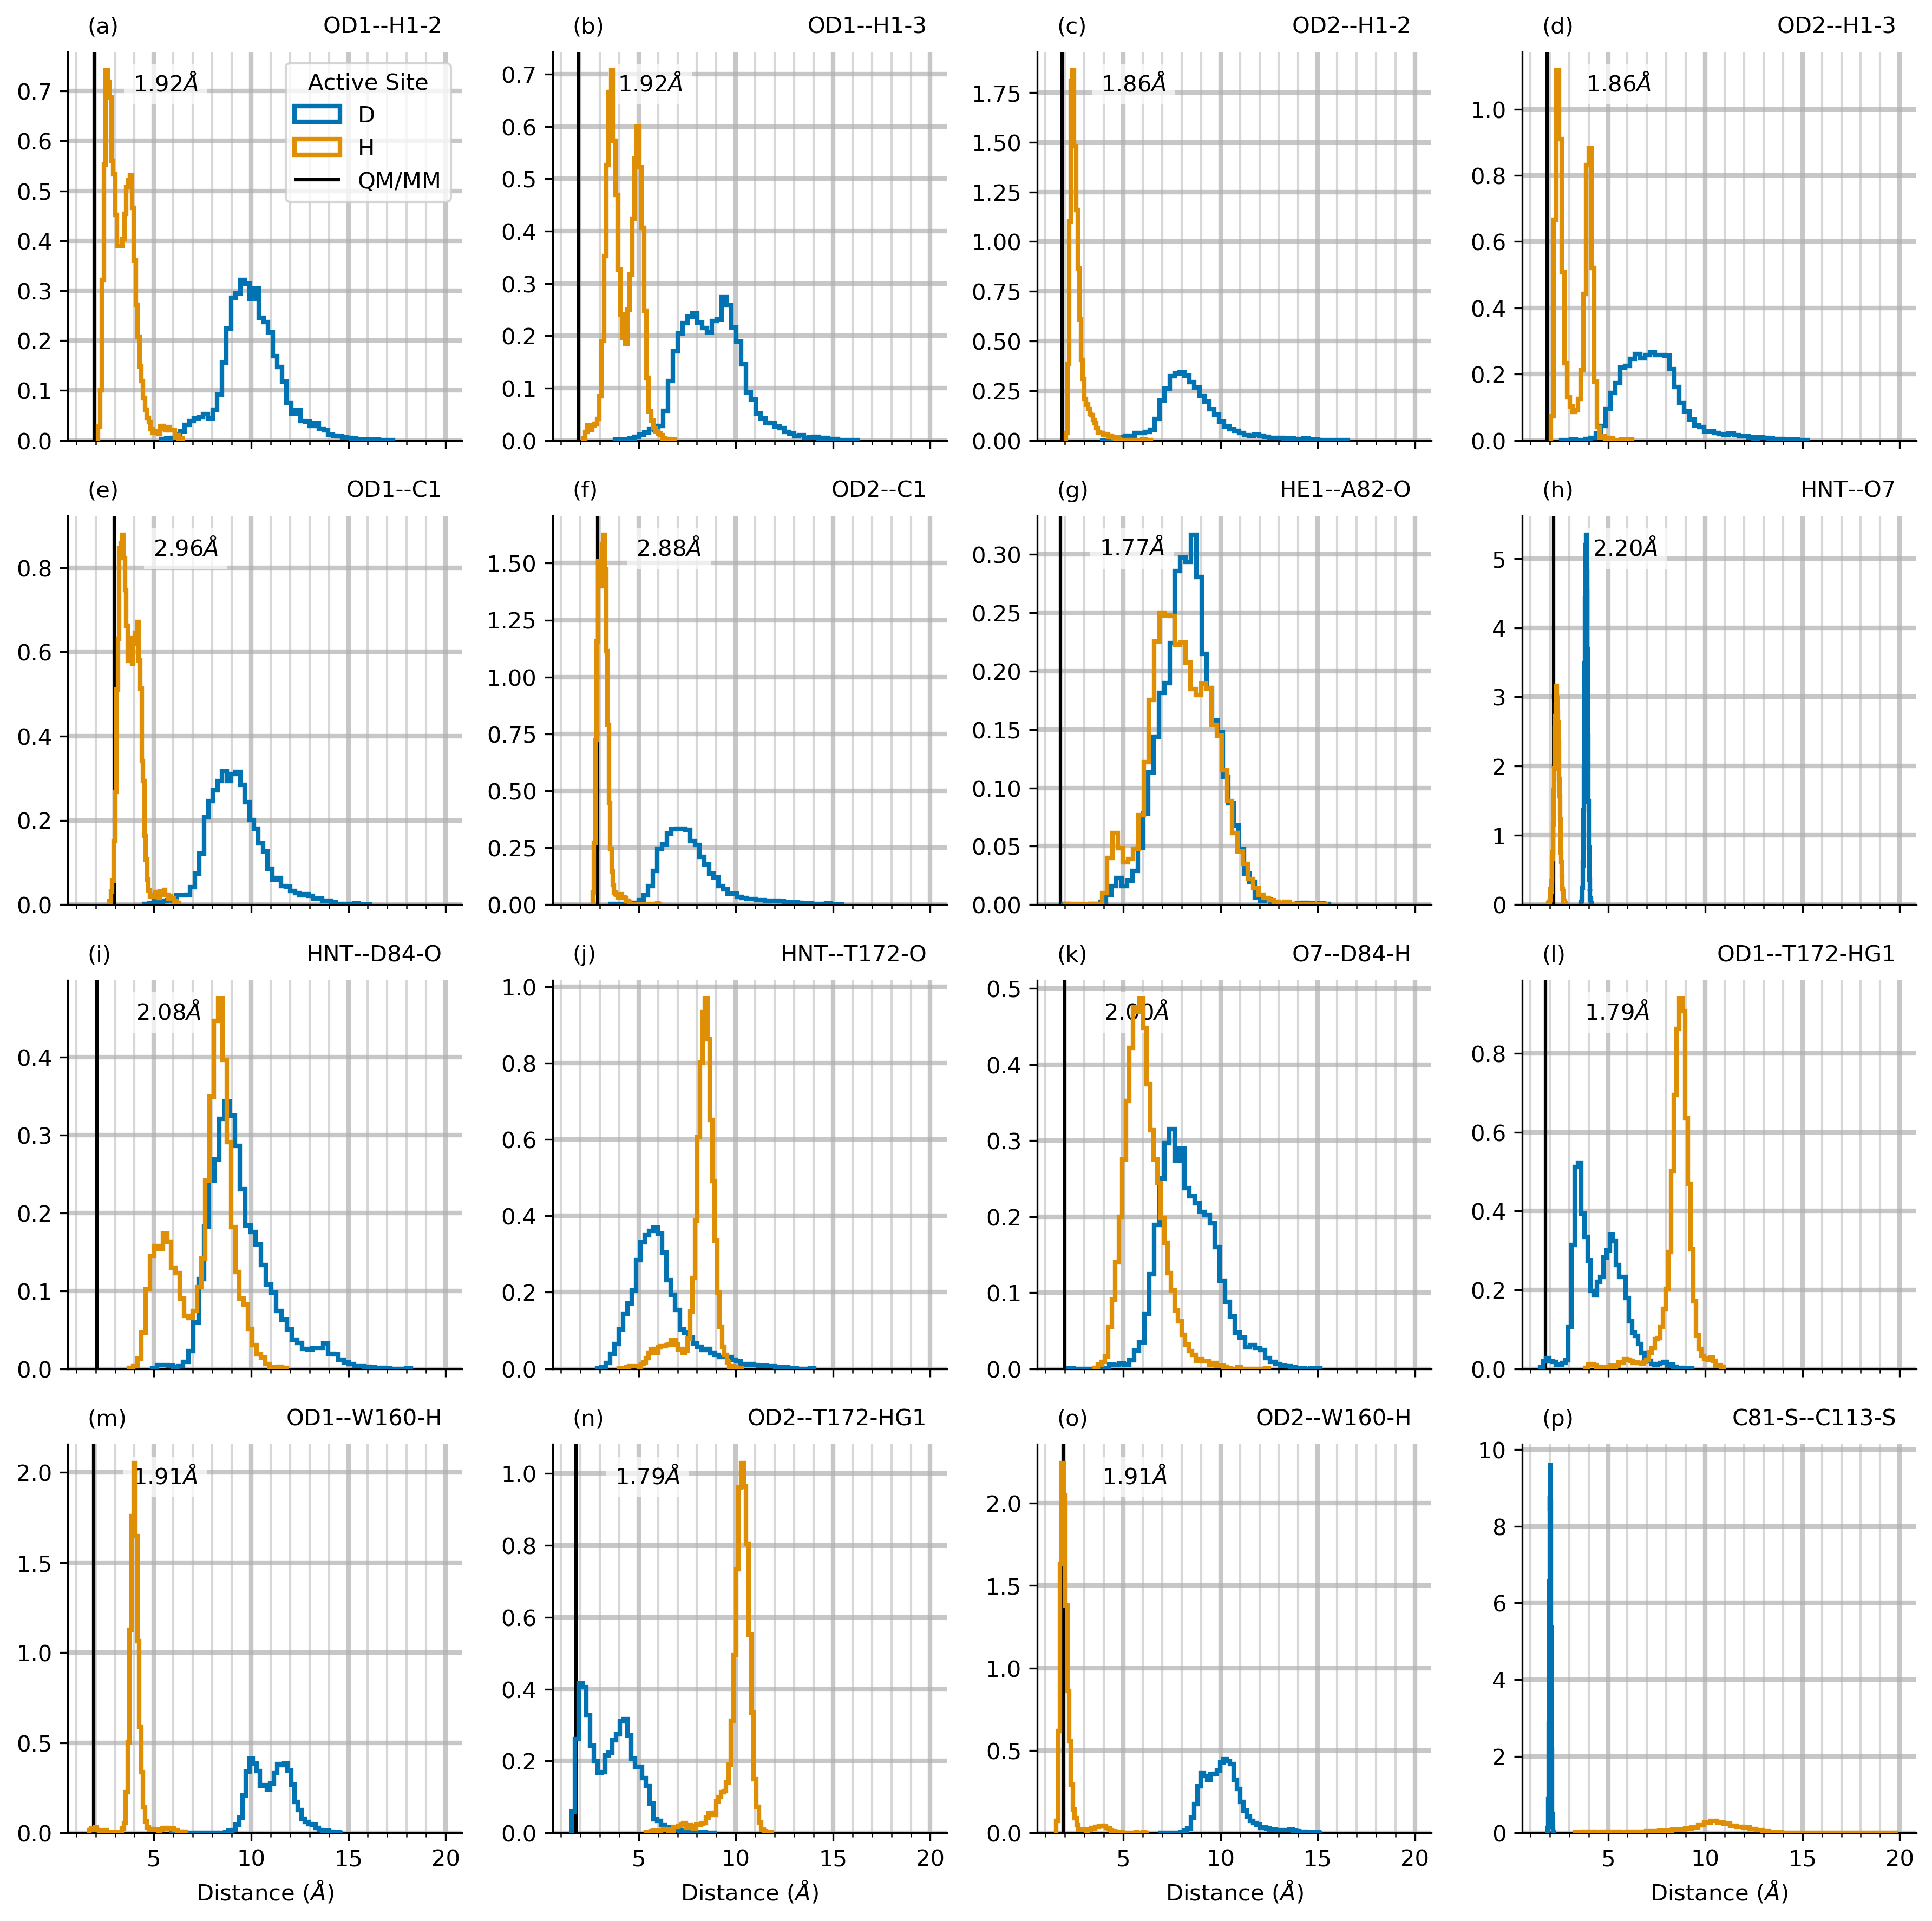
\includegraphics[width=0.8\textwidth]{chapters/aadh/figures/bond_distances_dist.png}
    \label{fig:bond_dist}
\end{figure}

To understand this difference between the active sites further and to explore the similarities between these simulations and previous work\cite{ranaghanInitioQMMM2017}, the distribution of important interatomic distances were calculated and compared. Figure \ref{fig:bond_dist} shows these bond distributions in blue for the D active site and in orange for the H active site. The black vertical lines with labels are the QM/MM interatomic distances in the reactant state\footnote{An average over the pathways to OD1 and OD2 are taken where appropriate.}, taken from table 3 of reference \cite{ranaghanInitioQMMM2017}. Where possible  the atom labels have been kept the same as those in reference \cite{ranaghanInitioQMMM2017}, the exceptions are the atoms directly involved in bond breaking and formation. The correspondence between the interatomic distances in reference \cite{ranaghanInitioQMMM2017} and figure \ref{fig:bond_dist}, and their description are as follows: 
\begin{enumerate}
    \item OD1/OD2---H1:  The bond being formed. These correspond to all four combinations of distances between OD2/OD1 (respectively) and H1-2, H1-3. Shown in panels (a) through (d). 
    \item OD1/OD2---C1: The donor/acceptor distance. These are the two combinations of distances between OD2/OD1 (respectively) and C1. Shown in panels (e) and (f). 
    \item HE1---A82-O: inter-residue hydrogen bond between HE1 of the TTQ prosthetic group and the Ala82 backbone oxygen atom, shown in panel (g). 
    \item HNT---O7: intra-residue hydrogen bond in the TTW residue. Shown in panel (h).
    \item HNT---D84-O: inter-residue hydrogen bond between the TTW residue and the backbone oxygen atom of the Asp84 residue. Shown in panel (i)
    \item HNT---T172-O: inter-residue hydrogen bond between TTW and the backbone oxygen atom in Thr172. This is not described in reference \cite{ranaghanInitioQMMM2017} but is included because of its potential to form a hydrogen bond in certain conformations. Shown in panel (j). 
    \item O7---D84-H: inter-residue hydrogen bond between the TTW residue and the backbone amide hydrogen atom of the Asp84 residue. Shown in panel (k). 
    \item OD1---T172-HG1/W160-H: The inter-residue hydrogen bond between the acceptor oxygen atom OD1 of D128 and hydrogen atoms on the Thr172 and Trp160 residues respectively. Shown in panels (l) and (m).
    \item OD2---T172-HG1/W160-H: The inter-residue hydrogen bond between the acceptor oxygen atom OD2 of D128 and hydrogen atoms on the Thr172 and Trp160 residues respectively. Shown in panels (n) and (o).\label{o1_t172}
    \item C81-S---C113-S: The sulphur-sulphur distance corresponding to the missing disulphide bond in the H chain. Shown in panel (p). \label{cs_cs} 
\end{enumerate}

In general, the bond lengths in the D active site show greater variance and do not, in general, overlap with those in the H active site. The main exception to this are the from the Cysteine residues 81 and 113. These have clearly drifted apart due to the lack of disulphide bond: the distribution of the S---S distances in the H active site, shown in panel (p) varies between \SIrange{3}{20}{\angstrom} compared to the effectively fixed distance of $\simeq \SI{2}{\angstrom}$ in the D active site. 

The O---H distances are smaller, closer to the QM/MM values, and show less variation in the H active site compared to the D active site by a significant margin (panels (a) - (d)). The distances in the H site are almost all less than \SI{5}{\angstrom} (within $\simeq\SI{3}{\angstrom}$ of the QM/MM values), where almost all the D active site values are between \SIrange{5}{10}{\angstrom}. The donor/acceptor distances, C---O (panels (e) and (f)) show a similar story. The closest hydrogen atom to both acceptor oxygen anions in the H active site is H1-2, the differences in the D active site are less obvious. These differences are due to the crystal structure preparation,  missing disulphide bond, and potentially due to conformational changes in loop residues \num{92}{108}, as: i) there is no difference between the active sites in the crystal structure (the difference in heavy atom RMSD  $<\SI{0.01}{\angstrom}$); and ii) the broken disulphide bond is incompatible with the pathways determined in references \cite{masgrauTunnelingClassicalPaths2007, ranaghanInitioQMMM2017}. 

There is no conclusive similarity between the QM/MM results and these simulations with respect to the stabilization of OD1 and OD2 by Thr172 and Trp160 by hydrogen bonds. This is important as it is these hydrogen bonds which help define the difference in between the hydrogen abstraction pathways. The orientation of Trp160-H, OD2, OD1 and Thr172-HG1 in the crystal structure and QM/MM is approximately linear. For OD1 to be hydrogen bonded with Thr172, the bond lengths would be ordered OD1---Thr172-HG1 $<$ OD1-Trp160-H, i.e. panel (l) $<$ panel (m). This is true for D but not for H. While for OD2 to be hydrogen bonded with Trp160, the bond lengths would be ordered OD2---Thr172-HG1 $>$ OD2-Trp160-H, i.e. panel (n) $>$ panel (o). This is true for H but not for D. In the D active site, Asp128 has moved away from Trp160 entirely but remained close to Thr172 as seen by comparing the distributions in  panels (m) and (o)  with panels (l) and (n). Noting that TTW is covalently bonded to Trp160, this is then consistent with the picture in panels (a) through (f) where OD1 and OD2 are between \SIrange{5}{15}{\angstrom} from the relevant atoms on TTW.  

The TTW intra-residue hydrogen bond, HNT---O7, shows good agreement with the QM/MM value in the H active site, while in the D active site it is larger by almost \SI{2}{\angstrom}. The two distinct HNT---O7 bond lengths define whether the NT---C1 bond is either syn or anti the C---O7 carbonyl bond in the tryptophan ring system of TTQ. The anti conformation, with has the shorter HNT---O7 distance, is adopted in active site H and in the crystal structure as shown in figure \ref{fig:aadh_active_site}.  Here the NT---HNT bond points in the same direction as the C---O7 bond and forcing the NT---C1 bond into the anti-conformation. The syn conformation has the has the NT---HNT bond pointing in the opposite direction, forcing the NT---C1 bond to eclipse the the C---O7 carbonyl bond. 

The syn and anti conformations allow radically different conformational states to be accessed as demonstrated in figure \ref{fig:ttw_wiggle}. Each panel shows \num{500} configurations, selected evenly across all trajectories, for the D (panel (a)) and H (panel (b)) active sites. The entire TTW residue and carbonyl group of Asp128 is shown and the conformations have been aligned to the tryptophan part of the TTW residue. The only two hydrogen atoms shown are H1-2 \& H1-3 and are coloured white. The syn conformation of the D active site clearly demonstrates a `looser' set of conformations with the  C1-H1 bond pointing away from the acceptor Asp128 residue, although whether this is due to missing disulphide bond or loop \num{92}{108} has not been determined. The anti conformation of the H active site shows a `tighter' set of conformations with the C1-H1 bond pointing towards the Asp128 residue. 

\begin{figure}
    \centering
    \mycaption[Conformations of the TTW residue in the D and H active sites]{\textsc{Conformations of the TTW residue in the D and H active sites}. Five conformations were taken from each trajectory at intervals of \SI{20}{\nano\second} and aligned along the heavy atoms of the trypotophan part of the TTW residue.  The hydrogen atom shown is the donor atom, all other hydrogen atoms are hidden.}
    \subbottom[Active site D]{
    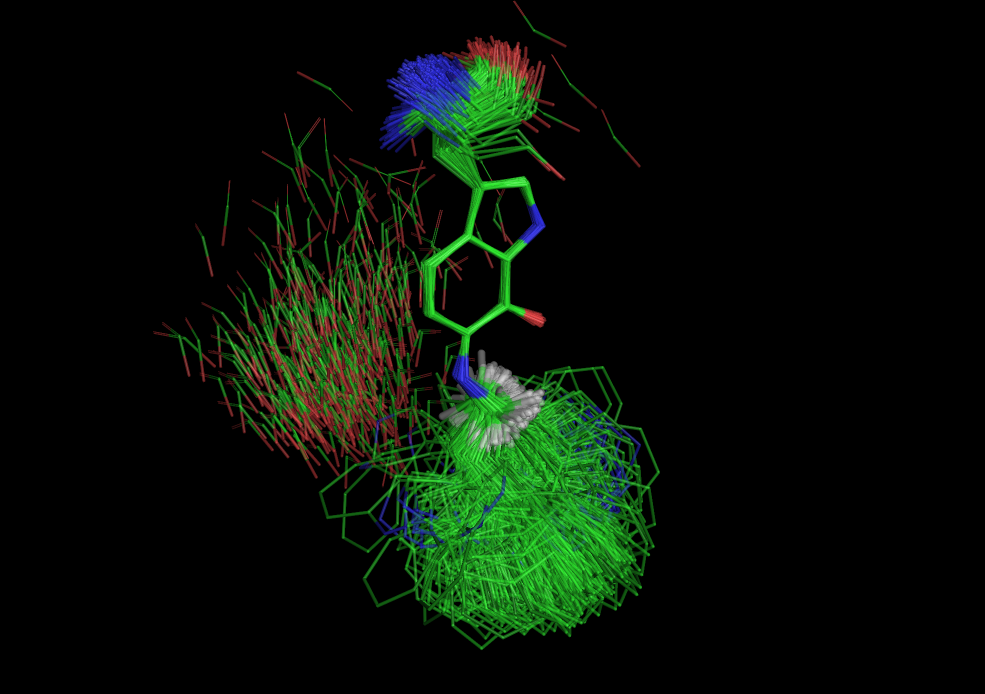
\includegraphics[trim={1cm, 0, 1cm, 0}, clip=True]{chapters/aadh/figures/as_d_wiggle.png}}
    \subbottom[Active site H]{
    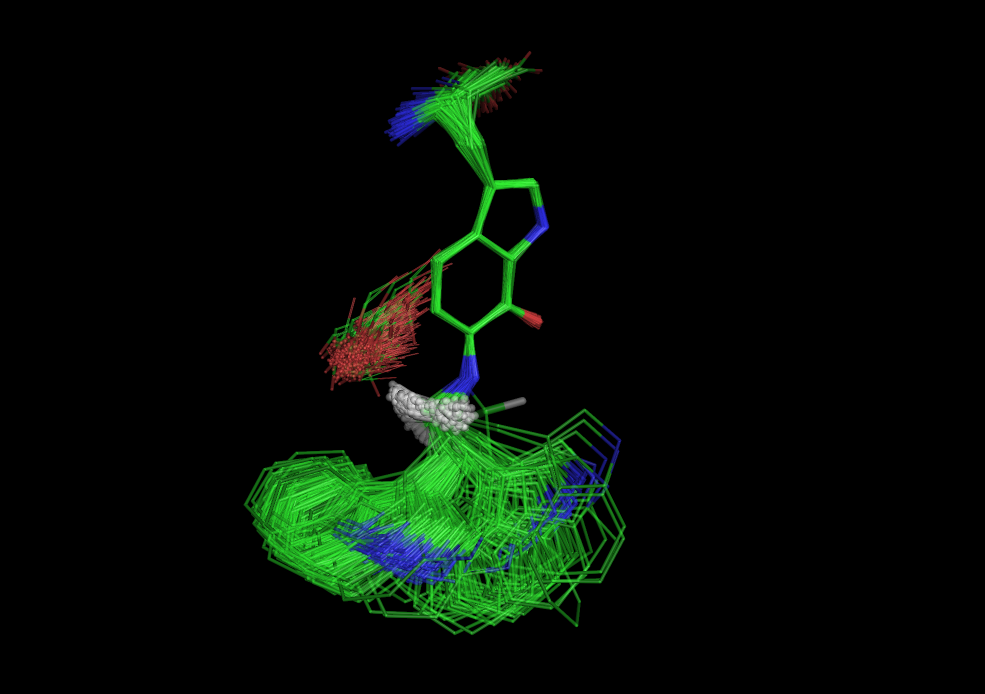
\includegraphics[trim={1cm, 0, 1cm, 0}, clip=True]{chapters/aadh/figures/as_h_wiggle.png}
    }
    \label{fig:ttw_wiggle}
\end{figure}

In summary, the two active sites show distinct differences in their accessible conformations. The missing disulphide bridge between residues Cys81 and Cys113 invalidates the trajectories of the H active site. However, it is not clear whether this missing bond can explain the difference in conformations between the two sites or whether this is due to the loop \numrange[range-phrase=-]{92}{108} dynamics. The two sites are differentiated in three main ways. First, the relevant interatomic distances and hydrogen bonds between TTW and Asp128 are more consistent with the QM/MM results in the H than in the D active site. Second, the orientation of the NT---C1 bond is syn the C---O7 carbonyl bond in the D active site, and anti in the H active site and QM/MM results. Third, the H site is more constrained with less variation in the available conformations compared to the  D active site. The apparent greater compatibility of the H active site with QM/MM results is surprising given the missing disulphide bridge occurs in the H active site. Despite this, only the trajectories for the D active site will be used in all further analysis.  

\section{MSM optimisation}\label{sec:aadh_optimisation}

The aim of this section is to create an optimised Markov state model of the active site of AADH using Bayesian optimisation and response surface methods developed in chapter \ref{chap:msm}. In addition, to test the robustness of the modelling procedure a sensitivity analysis based on the response surface of the MSM will be produced. This section proceeds in four steps: first in subsection \ref{sec:aadh_est_tau_k}, a suitable  value of the Markov lag time $\tau(\mathrm{MSM})$, and number of slow relaxation processes, $k$ will be estimated using a reference MSM. These will be used to specify the MSM and the VAMP-2 score so that in the second step, subsection \ref{sec:aadh_rsm},  the MSM response surface can be modelled as a Gaussian process (GP). Third, using this model of the response surface Bayesian optimisation will be used to determine the optimal set of hyperparameters, these will constitute the base case model.  In the fourth step, subsection \ref{sec:aadh_sens_analysis}, a number of alternate models will be proposed (`sensitivity 1, 2' etc.)  using knowledge of MSM response surface and eigenvalue spectrum.  

\subsection{Estimating Markov lag-time and number of metastable states}\label{sec:aadh_est_tau_k}

% The conformational dynamics and metastable states of the active site of AADH will be explored later chapters. In particular, chapter \ref{chap:msm} will detail the how to choose the trajectory pre-processing choices (hyperparameters) to estimate an optimal MSM. This requires fitting and evaluating a number of MSMs which in turn requires the specification of a Markov lag time ($\tau(\mathrm{MSM})$) and the number, $k$, of dominant eigenvalues. 
Suitable values of the Markov lag-time, $\tau(\mathrm{MSM})$, and  the number of dominant relaxation processes, $r$, were estimated by inspection of the eigenvalue spectrum of a reference MSM. The following results are for the D active site only as the missing disulphide bond in the H active site rendered these trajectories invalid.

The trajectories were discretized by first projecting the cartesian coordinates onto a set of features, applying TICA to reduce the dimension of the feature space and then clustering the frames into a small set of discrete states.  The features used were the bond lengths identified in reference \cite{ranaghanInitioQMMM2017} i.e., those whose histograms are depicted in panels (a) - (g), (i), (k), (l), (o) of figure \ref{fig:bond_dist}. The intramolecular hydrogen bond in panel (h), originally included in reference \cite{ranaghanInitioQMMM2017}, was excluded due to its small variance. The trajectories were strided to give a trajectory time-step \SI{0.1}{\nano\second}. TICA was applied with a lag time of $\tau=\SI{1}{\nano\second}$ and the number of components set so as to retain \SI{95}{\percent} of the kinetic variance. This equated to retaining $m=10$ components. k-means clustering was used to cluster the trajectories into $n = 316$ microstates states. The number of microstates was chosen as the square root of the number of observations, inline with the heuristic in reference  \cite{husicWardClusteringImproves2017a}. 

The Markov lag time must be chosen large enough so that the Markov assumption holds. This equates to the implied timescales:
\begin{equation*}
    t_{i}=-\frac{\tau(\mathrm{MSM})}{\ln{|\lambda_{i}|}}, 
\end{equation*} 
being independent of $\tau(\mathrm{MSM})$. However, the eigenvalue spectrum will be heavily influenced by choice of hyperparameters, in particular the protein feature. So a suitable lag time for this particular set of hyperparameters may not prove suitable for another set. In other words, a suitable lag time cannot be chosen independent of the hyperparameters, but the hyperparameters cannot be optimised without specifying a lag time. The same reasoning also applies to the number of dominant eigenvalues used in the VAMP-2 score. 

\begin{figure}
    \centering
    \mycaption[The implied timescales and relative VAMP-2 scores as a function of the Markov lag time]{\textsc{The implied timescales and relative VAMP-2 scores as a function of the Markov lag time $\tau(\mathrm{MSM})$}. The TICA lag time was $\tau=\SI{1}{\nano\second}$ with $m=10$ components retained. The number of cluster centres was $n=316$. Panel (a) shows the first five implied timescales for $\tau(\mathrm{MSM})=\SIrange[range-phrase=-]{0}{5}{\nano\second}$, panel (b) shows the first five implied timescales for $\tau(\mathrm{MSM}) = \SIrange[range-phrase]{0}{50}{\nano\second}$. The solid lines and coloured shaded areas are the mean and \SI{95}{\percent} credible intervals respectively, estimated using MCMC with \num{500} posterior samples. The grey shaded area is the region for which the implied timescales are smaller than the lag time. Panel (c) and (d) show the VAMP-2 scores, scored on the first \numrange{2}{5} eigenvalues for the same ranges. The VAMP-2 scores are indexed to their value at $\tau(\mathrm{MSM})=\SI{0.1}{\nano\second}$. The colour coding is consistent between the implied timescale plots ((a) and (b)) and VAMP-2 plots ((c) and (d)). e.g. the blue line in (c) and (d) is the VAMP-2 score with two eigenvalues ($r=2$) while in (a) and (b) blue is the second implied timescale, $t_{2}$. }
    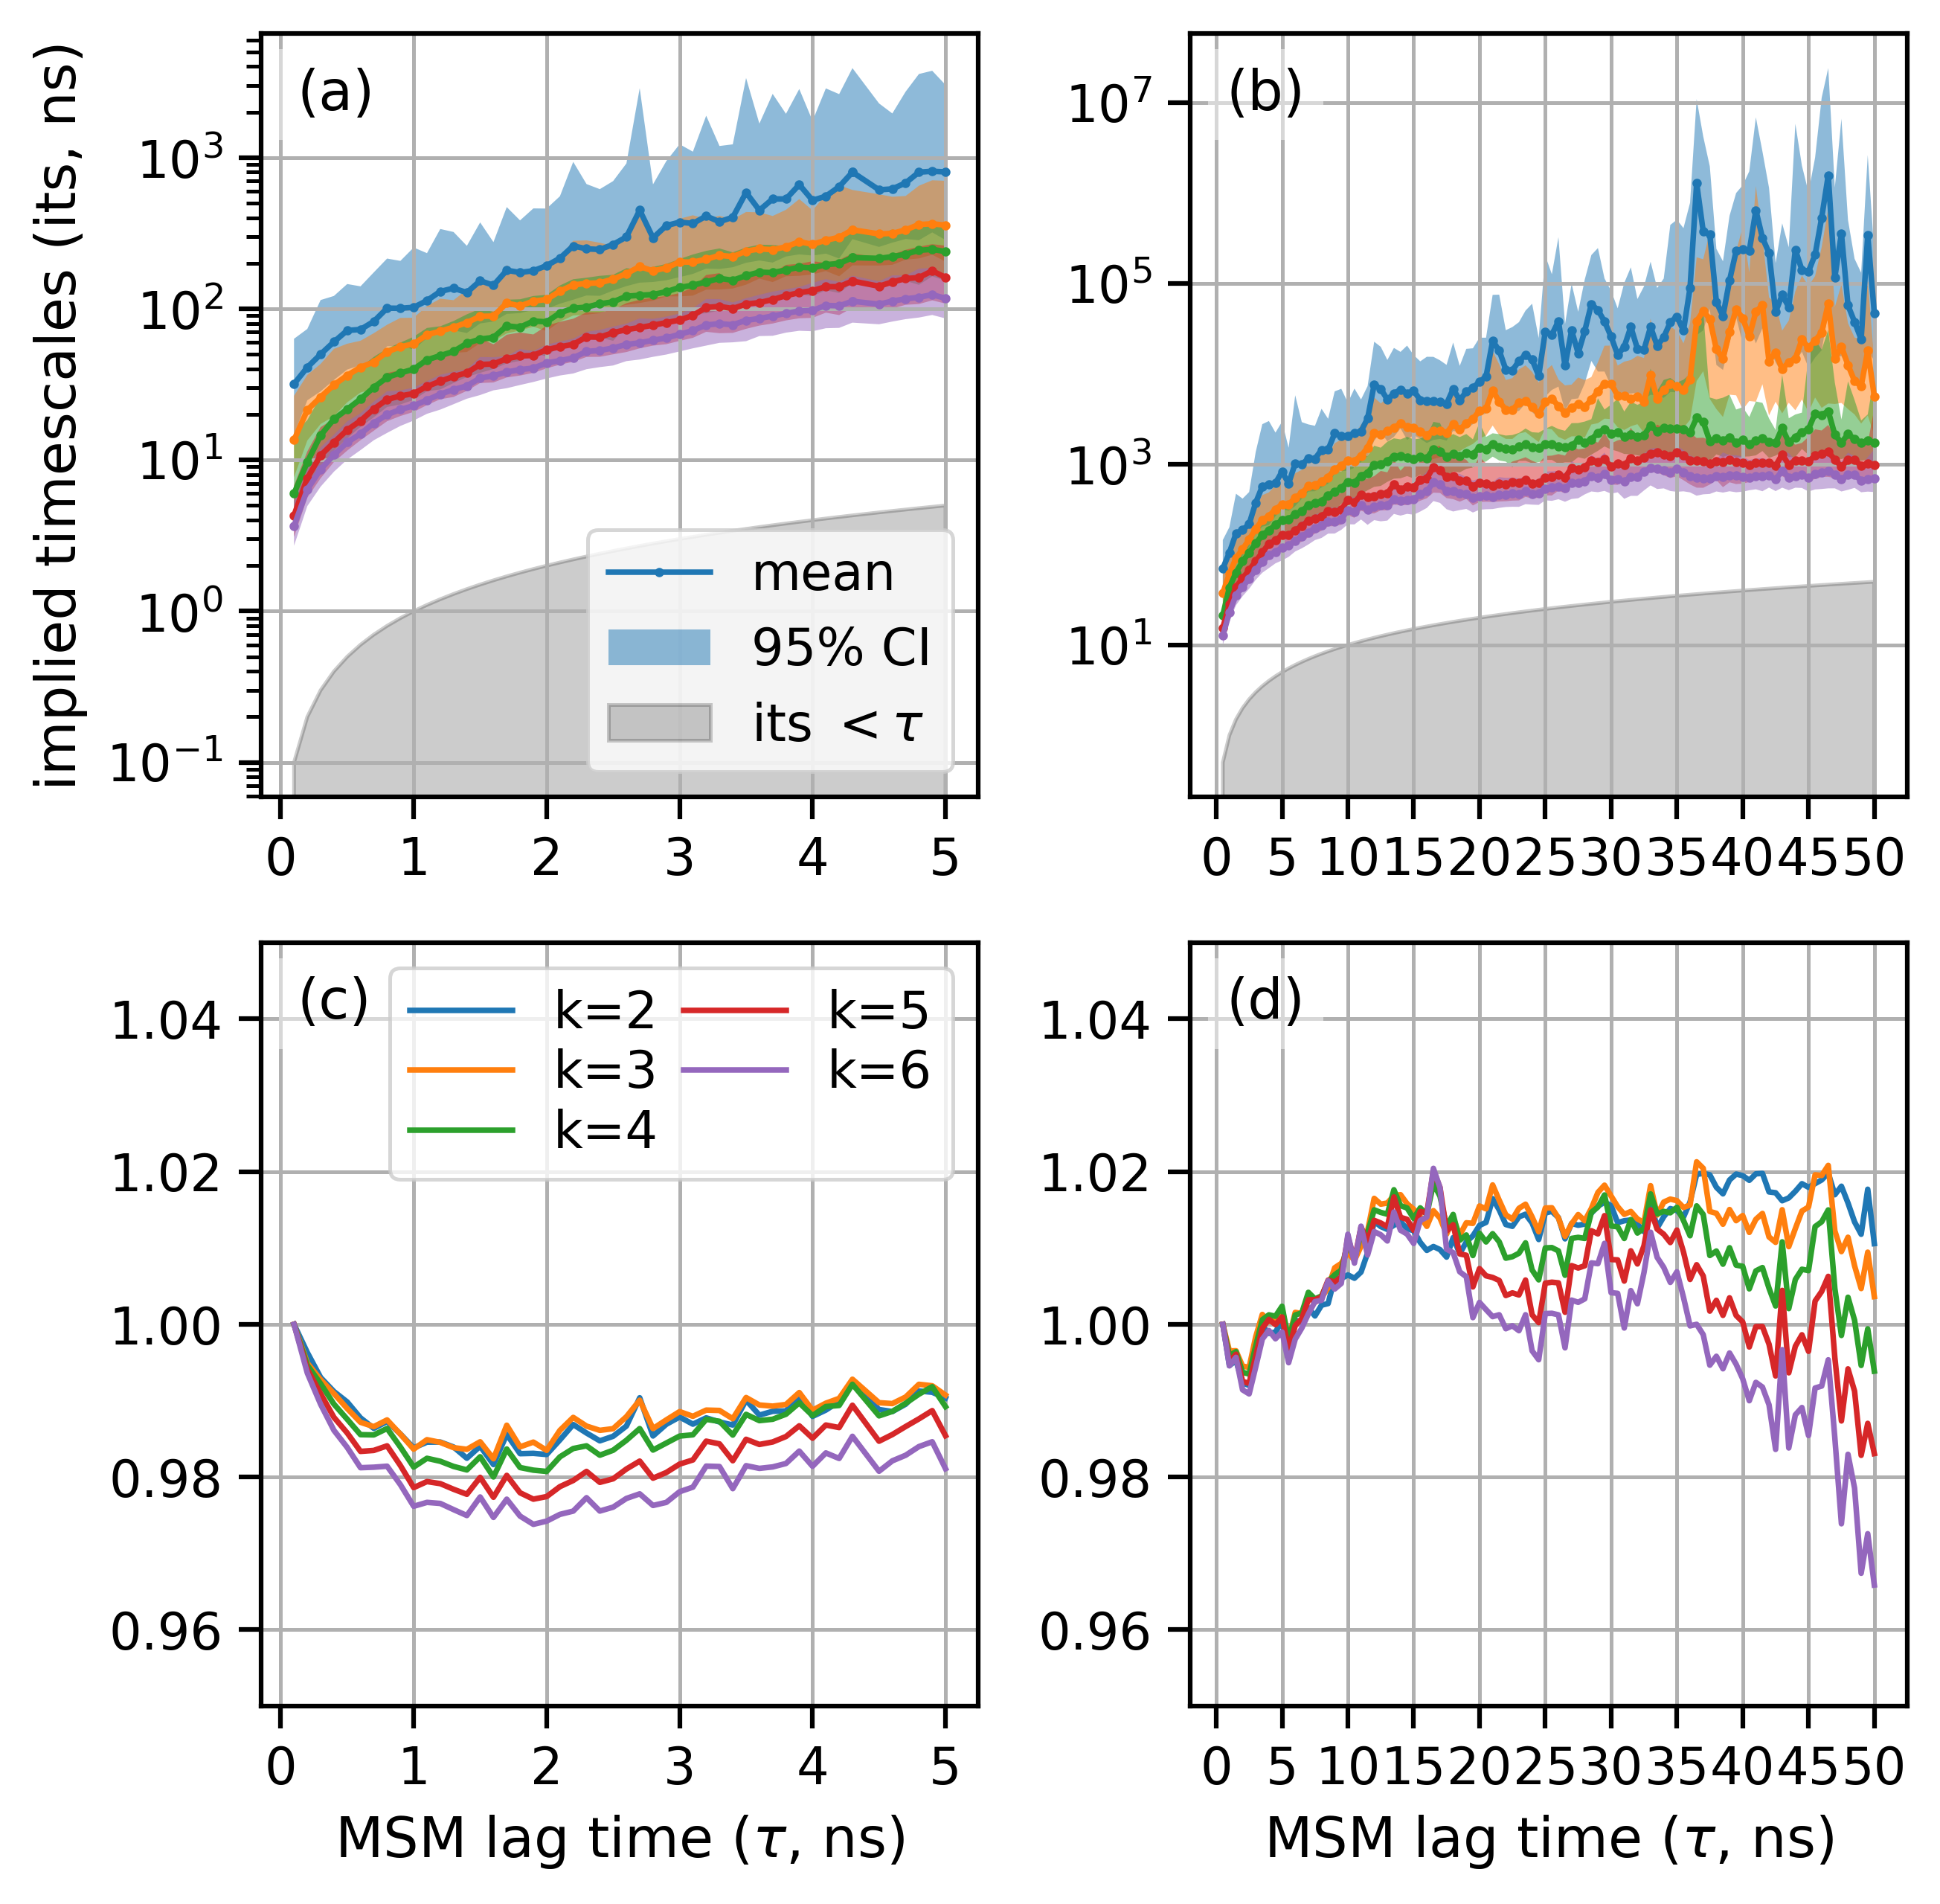
\includegraphics[width=0.8\textwidth]{chapters/aadh/figures/implied_timescales_D.png}
    \label{fig:its_d}
\end{figure}

A way out of this circular reasoning problem can be found by noting the following. First, the purpose of specifying the lag time and number of dominant processes is to provide a starting point from which the hyperparameters of the MSM can be optimised. It is therefore only necessary that the choice of $\tau(\mathrm{MSM})$ do not affect the optimisation, rather than provide a strictly valid MSM specification. The lag time and number of dominant relaxation processes has only a small effect on the value of the VAMP-2 score as demonstrated by figure \ref{fig:its_d}. The first five implied timescales are shown a panel (a)  for $\tau(\mathrm{MSM})$ in the range \SIrange{0}{5}{\nano\second} and panel (b) for $\tau(\mathrm{MSM})$ in the range \SIrange{0}{50}{\nano\second}. Underneath, in panels (c) and (d) are shown the VAMP-2 scores with $r$ ranging from \numrange{2}{5}, which correspond to successively including the implied timescales shown in panels (a) and (b). The implied timescale (shown in blue) appears to become independent of the lag time from approximately \SI{12}{\nano\second}. However as panels (c) and (d) show the lag time has little effect on the VAMP-2 scores which vary by less than $\pm\SI{4}{\percent}$ from their initial values over all lag times. The value of $r$ also has little effect on VAMP-2 scores, at least up to $\tau(\mathrm{MSM})=\SI{15}{\nano\second}$ where their relative values start to diverge. Third, a value of $\tau(\mathrm{MSM})$ and $r$ used for inference can be determined after optimisation through appropriate sensitivity analysis. A value of $\tau(\mathrm{MSM})=\SI{2}{\nano\second}$ was chosen based on the relatively small variation of the VAMP-2 score (panel (c) of figure \ref{fig:its_d}) and the larger number of observations that a small value affords. 

\begin{figure}
    \centering
    \mycaption[The ratio of successive eigenvalues and implied timescales of the reference MSM]{\textsc{The ratio of successive eigenvalues and implied timescales of the reference MSM}. Panel (a) shows the ratio of eigenvalues and panel (b) the implied timescales for the reference MSM with $\tau(\textrm{MSM})=\SI{2}{\nano\second}$, estimated using MCMC with \num{1000} posterior samples. The TICA lag time was  $\tau=\SI{1}{\nano\second}$, with \SI{95}{\percent} of the variance ($m=10$ components) retained. The number of cluster centres was $n=316$. The blue dots and error bars are the mean and \SI{95}{\percent} credible intervals.}
    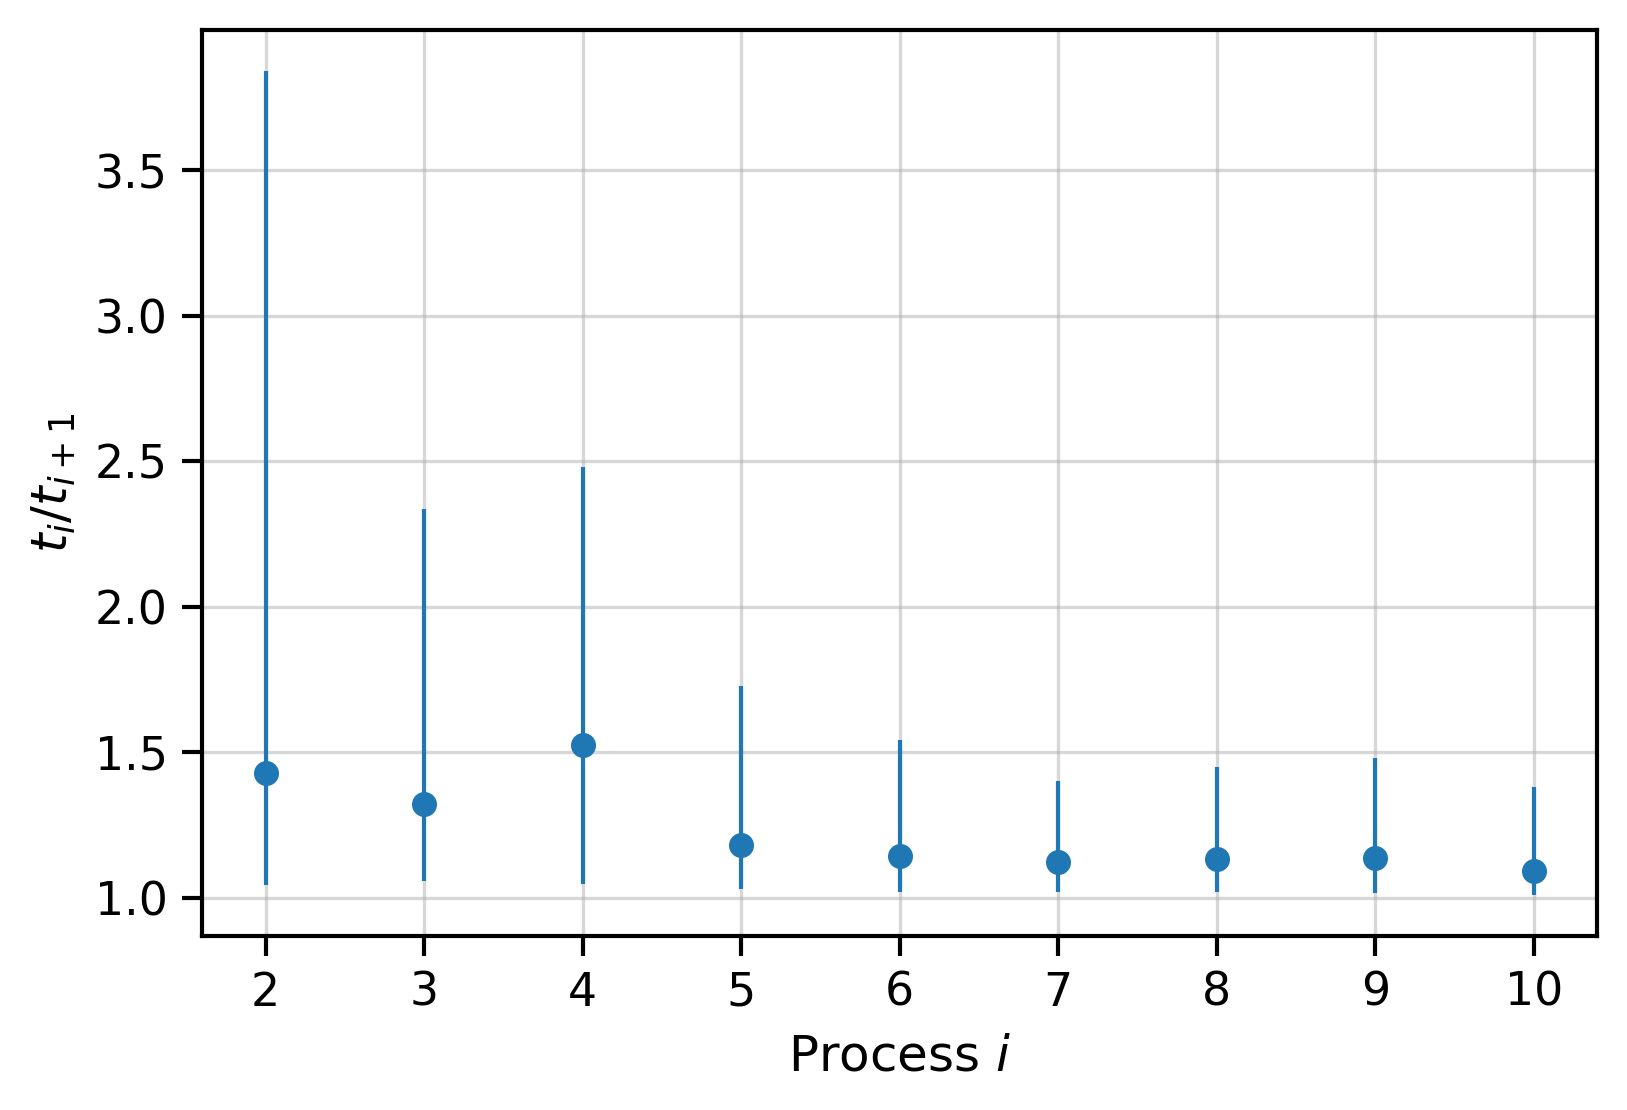
\includegraphics[width=0.8\textwidth]{chapters/aadh/figures/timescale_ratios_D.png}
    \label{fig:ts_ratios_d}
\end{figure}

There were no significant gaps in eigenvalues at $\tau(\mathrm{MSM})=\SI{2}{\nano\second}$  shown figure \ref{fig:ts_ratios_d} panel (a). So the number of dominant processes was determined by inspection of the relative gaps in the timescale spectrum shown in  panel (b). The largest timescale separation was between the fourth and fifth relaxation process, suggesting a value of $r=4$. 

An alternative analysis was performed using a TICA lag time of $\tau=\SI{10}{\nano\second}$ with \SI{95}{\percent} of the variance ($m=8$ components) retained with same number of cluster centres, $n=316$. The implied timescale plots are shown in figure \ref{fig:its_d_sens} and  do not change the Markov lag time suggestion of \SI{2}{\nano\second}. The ratio of eigenvalues and implied timescales  are shown in figure \ref{fig:ts_ratios_d_sens}. There was no clear separation in either the eigenvalues or the implied timescales and so the value of $4=4$ from reference MSM was retained.

\subsection{Response surface}\label{sec:aadh_rsm}

\begin{table}[h]
    \mycaption[The hyperparameter search space for AADH]{\textsc{The hyperparameter search space for AADH}. TICA was applied to every feature except RMSD. Dihedral angles, $\theta$, were given $(\sin(\theta),\cos(\theta)$ representations to account for their periodicity.  The Cartesian coordinates were first aligned to a single, randomly chosen, trajectory frame so that feature (5) did not include spurious rotational or translational motion. The number of dimensions, `Dim.', refers to the number of individual feature variables created by $\chi$.}
    \centering
    \begin{tabularx}{0.9\textwidth}{ |>{\raggedright\arraybackslash}l|l|>{\raggedright\arraybackslash}X|c| >{\raggedright\arraybackslash}X | } 
    \hline
    \textbf{Hyperparameter} & \textbf{Type} & \textbf{Range} & \textbf{Dim.} &\textbf{Details} \\
     \hline\hline
    Feature, $\chi$ & Categorical & (1) $(\phi, \psi, \chi)$ & $\num{116}$  & \\
    & & (2) $|\mathbf{r}_{1}-\mathbf{r}_{2}|$  & $\num{ 2346}$& Heavy atom interatomic distances \\
    & & (3) $C_{\alpha}-C_{\alpha}$ & $\num{15}$ & $\alpha$-carbon contacts\\ 
    & & (4) $X-X$  & $\num{15}$ & Heavy atom contacts\\ 
    & & (5) RMSD & $\num{1}$ &  Heavy atoms only\\ 
    \hline
    TICA lag time, $\tau$ & Integer &\SIlist[list-final-separator = { ... }]{1;1.1;100}{ns} &  & \\
    \hline
    TICA components, $m$& Integer &\numlist[list-final-separator = { ... }]{1;2;20} & & \\
    \hline
    Cluster centres, $n$ & Integer & \numlist[list-final-separator = { ... }]{10;11;1000}& &  Clustered using k-means clustering  \\
    
     \hline
    \end{tabularx}
    \label{tab:aadh_searchspace}
\end{table}

The response surface of an MSM for the active site of AADH was estimated using the same method for alanine dipeptide, detailed in chapter \ref{chap:msm}. A summary of this method applied to AADH is as follows. The MD data used were the $100$ coordinate trajectories of the six residues of the D active site of AADH defined in figure \ref{fig:aadh_active_site}. These trajectories were pre-processed into discrete states by first projecting onto a continuous feature $\chi$; applying TICA with a lag time of $\tau$ and retaining $m$ independent components (IC$1$, ..., IC$m$);  then clustering into $n$ discrete microstates using k-means clustering. Collectively these are the MSM hyperparameters $\mathbf{x} = (\chi, \tau, m, n)$. The range of possible values of $\mathbf{x}$, the hyperparameter search space, are shown in table \ref{tab:aadh_searchspace}. The $(\phi, \psi, \chi)$ feature  was the usual backbone and residue dihedral angles but augmented with the six dihedral angles joining the two \num{9} membered rings in the TTW residue. \num{500} different sets of hyperparameters were sampled from the search space (\num{100} per feature). To each value of $\mathbf{x}$ an MSM was fitted with a lag time of $\tau(\mathrm{MSM}) = \SI{2}{\nano\second}$ and the response, $y$, measured with VAMP-2 with $r=4$ eigenvalues using 20 iterations of 50:50 shuffle split (algorithm \ref{alg:shuffle_split}). The \num{500} pairs of hyperparameter/response measurements  constituted the hyperparameter trial data set, $\mathcal{D}_{500} = \{(\mathbf{x}_{i}, y_{i}),\ i = 1, \ldots, 500\}$. The response surface $f(\mathbf{x}; \mathcal{D}_{500})$, was modelled as a Gaussian process (GP), with covariance kernel and input warping selected using a combination of the mean standardized log-loss (MSLL) and the standardized mean square error (SMSE). The relevance of the hyperparameters were extracted, discussed, and also used to inform suitable visualisations of the response surface. 

\begin{figure}[p]
    \centering
    \mycaption[The VAMP-2 scores of the hyperparameter trials for MSMs of AADH]{\textsc{The VAMP-2 scores of the hyperparameter trials for MSMs of AADH}. The test response, $f^{test}=f\left(\mathbf{x}; \{s^{test}\}\right)$, is shown in blue, for (a) the $(\phi, \psi, \chi)$ dihedral angles, (c) heavy atom interatomic distances, (e) $\alpha$-carbon contact distances, (g) heavy atom contact distances, (i) root mean square deviation of heavy atoms. The difference between $f^{train}$ and $f^{test}$ is shown in orange for (b) the the $(\phi, \psi, \chi)$ dihedral angles and so on. The horizontal axis is the rank of the trial according to the test score. Each trial was scored with \num{20} iterations of 50:50 shuffle split cross-validation. The error bars represent the 25th and 75th quantiles of the cross-validation folds. The features are ordered according to the mean of the their test scores.}
    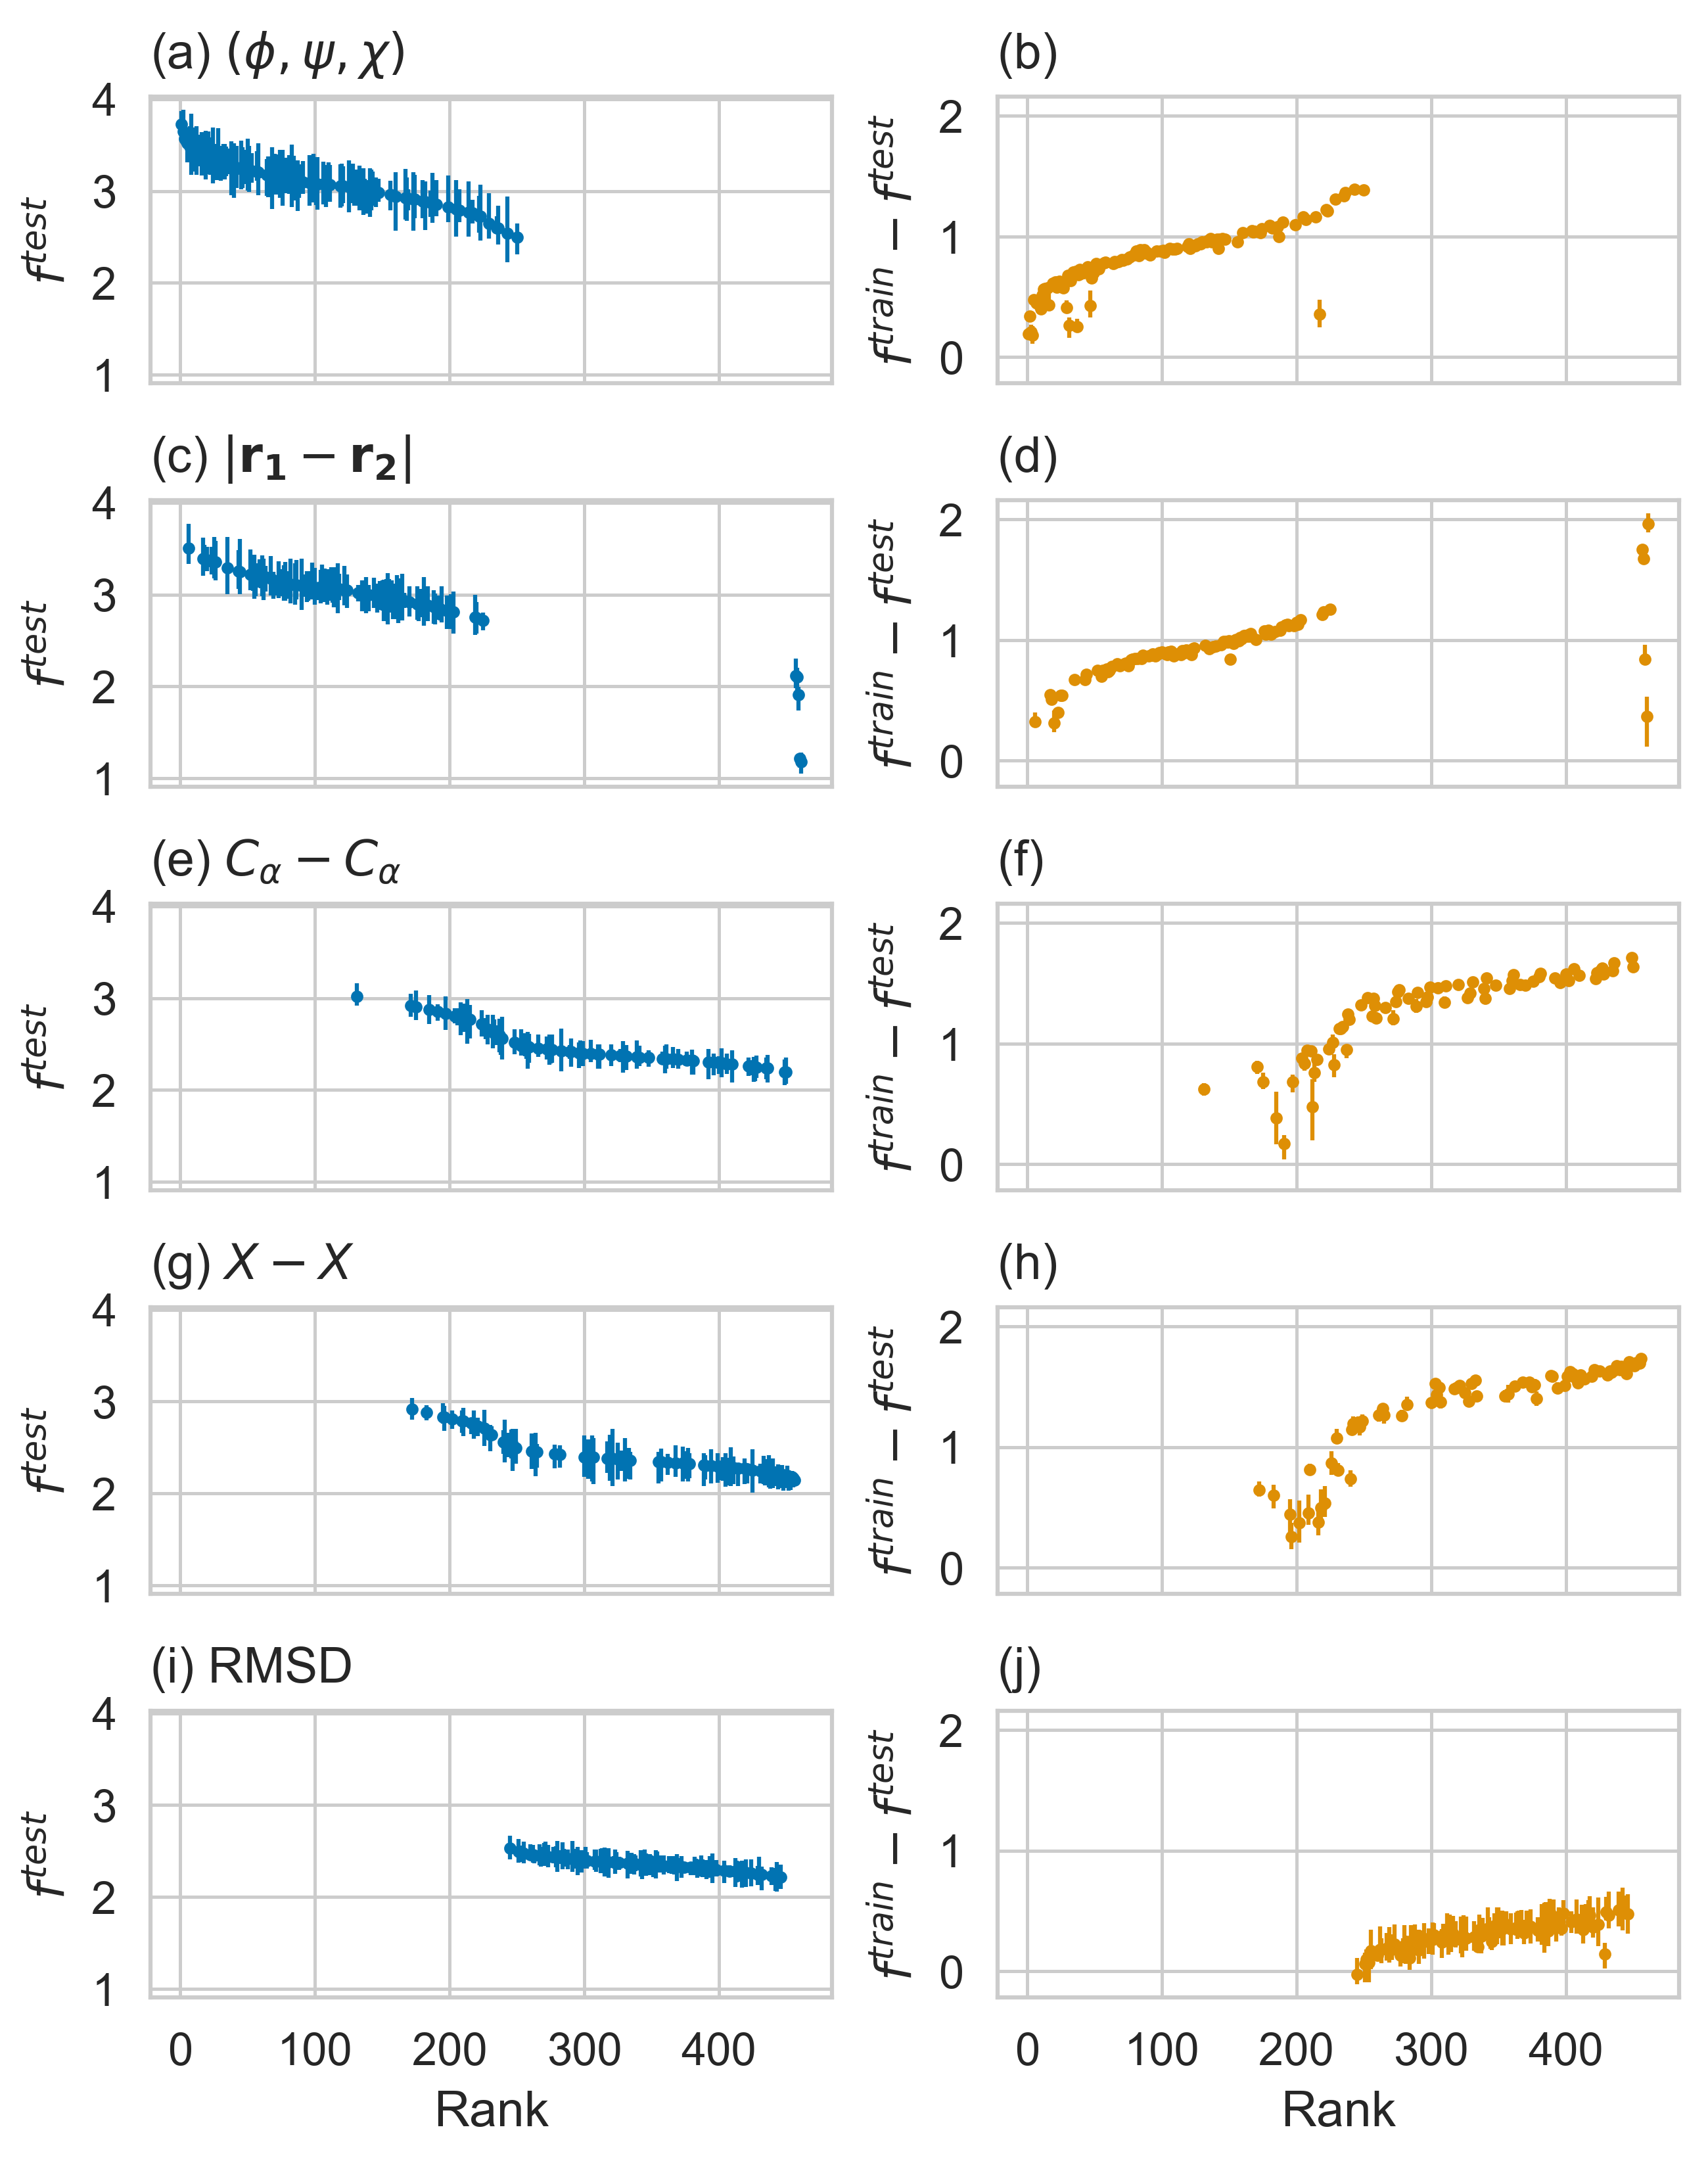
\includegraphics[width=0.8\textwidth]{chapters/msm_optimization/figures/aadh_train_test_results.png}
    \label{fig:aad_train_test}
\end{figure}

The hyperparameter trial data set, $\mathcal{D}_{500}$, is shown in figure \ref{fig:aad_train_test}. The mean test response is shown in blue and the difference between the training and test response shown in orange. Not all trials were successful (for example, if the number of TICA dimensions retained, $m$, exceeded the number of dimensions of the feature, $\chi$) and these trials were ignored in the following analysis, this resulted in a final trial data set of size $N=461$. The panels correspond to the value $\chi$ and are ordered according to their average of the test responses. The horizontal axis is the rank of the trial determined by their test response. There is clear range of response values in the range $2 < \operatorname{VAMP-2} < 4$ with the $(\phi, \psi, \chi)$ dihedral angles  (panel (a)) and the interatomic distances feature ( $\left|\mathbf{r}_{1}-\mathbf{r}_{2}\right|$) (panel (c)) both performing the best out of the five features. 

In contrast to the case of alanine dipeptide, all features show a marked degree of over-fitting $\Delta f$. However, within each feature there are combinations of the remaining hyperparameters for which $\Delta f=0$ implying that it is possible to create a consistent picture of relaxation processes which generalize well for each feature. The response of the $(\phi, \psi, \chi)$ feature  approaches the maximum response of $VAMP-2 = 4$ for the highest ranked trials, indicating the possibility of at least three slow relaxation processes. 

\begin{figure}
    \centering
    \mycaption[goodness-of-fit for the GP modelled response surface of AADH]{\textsc{goodness-of-fit for the GP modelled response surface of AADH}.  Panels (a) - (d) shows the goodness-of-fit conditional on each feature. The GP uses an exponential kernel with linear input warping on $\tau, m$ and $n$. The MSLL and SMSE were $-0.01298$ and  $0.3087$ respectively. The horizontal axis ($y$) are the observed trial values and the vertical axis is the mean response ($f(\mathbf{x})$). The error bars are $\pm 2\sigma$ where $\sigma$ is the standard deviation of the response surface including the noise term $\sigma_n$.}
    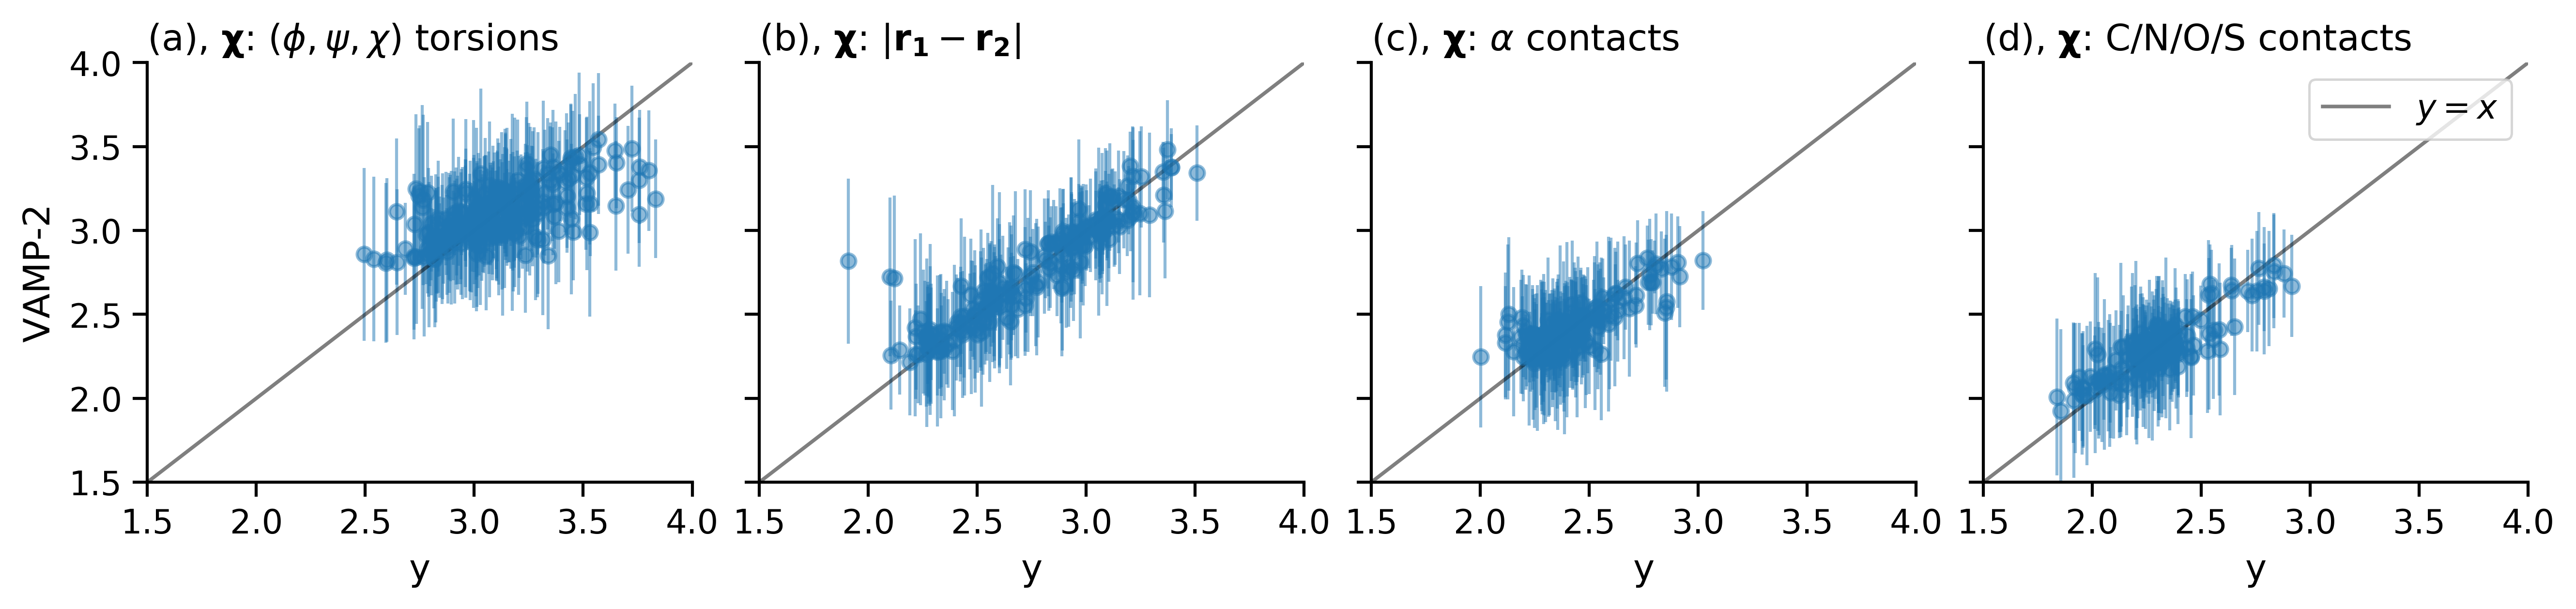
\includegraphics[width=0.8\textwidth]{chapters/msm_optimization/figures/aadh_response_surface_fit_d.png}
    \label{fig:aadh_rsm_fit}
\end{figure}

The response surface as a function of the feature, $\chi$, TICA lag time, $\tau$, number of TICA components retains $m$, and the number of cluster centres, $n$ was estimated with a GP. The RMSD feature trials were removed from data set because the $\tau$ and $m$ hyperparameters do not apply, which would have created a \emph{conditional} search space\cite{bergstraAlgorithmsHyperParameterOptimizationa} which  can't easily be modelled by GPs (there are attempts to mitigate this\cite{swerskyRaidersLostArchitecture2014}). While this is a problem in general for this method, the poor performance of RMSD as a feature both here and with alanine dipeptide means that this will not affect finding the optimum hyperparameters. There were also a number of trials which failed to converge an MSM, these were also removed. The final hyperparameter trial data set had $N=361$ observations, $\mathcal{D}_{361}$. 
The covariance kernel was chosen from amongst the same set as for alanine dipeptide: exponential, Mat\'{e}rn 3-2, Mat\'{e}rn 5-2 and  Gaussian (equations \ref{eqn:kern_exp} - \ref{eqn:kern_gauss}). In addition, the choice of logarithmic  input warping was optionally applied to $\tau$, $m$ and $n$. The best combination, based on their combined rank using the MSLL and SMSE metrics, was an exponential kernel and a linear input transformation for $\tau, m$ and $n$. See table \ref{tab:aadh_rsm_metrics_all_data} for  all the models' selection metrics. A more intuitive assessment of the fit of the can be found in figure  \ref{fig:aadh_rsm_fit} which shows the correlation between observed and predicted values for each feature. There is clearly a good fit for all the features except for $(\phi, \psi, \chi)$ where the predicted values are slightly under and over estimated for the highest and lowest values with this feature respectively. This creates the possibility of a false bimodal response surface which must be checked when determining the optimal hyperparameters.  The relatively poor fit on this feature is likely due to the fully multiplicative nature of the kernel. More flexible kernels (as discussed in e.g., reference \cite{duvenaud2011additive}) which model lower order interactions may be able to overcome this problem in future work. 

\begin{figure}
    \centering
    \mycaption[The relevance of the hyperparameters of AADH]{\textsc{The relevance of the hyperparameters of AADH}. The distribution of the parameters of the response surface were estimated using MCMC with \num{1000} posterior samples. The relevance of the features (levels of $\chi$) are shown in blue, labelled `Feature'. The relevance of the the other hyperparameters are shown in orange, labelled `Other'.}
    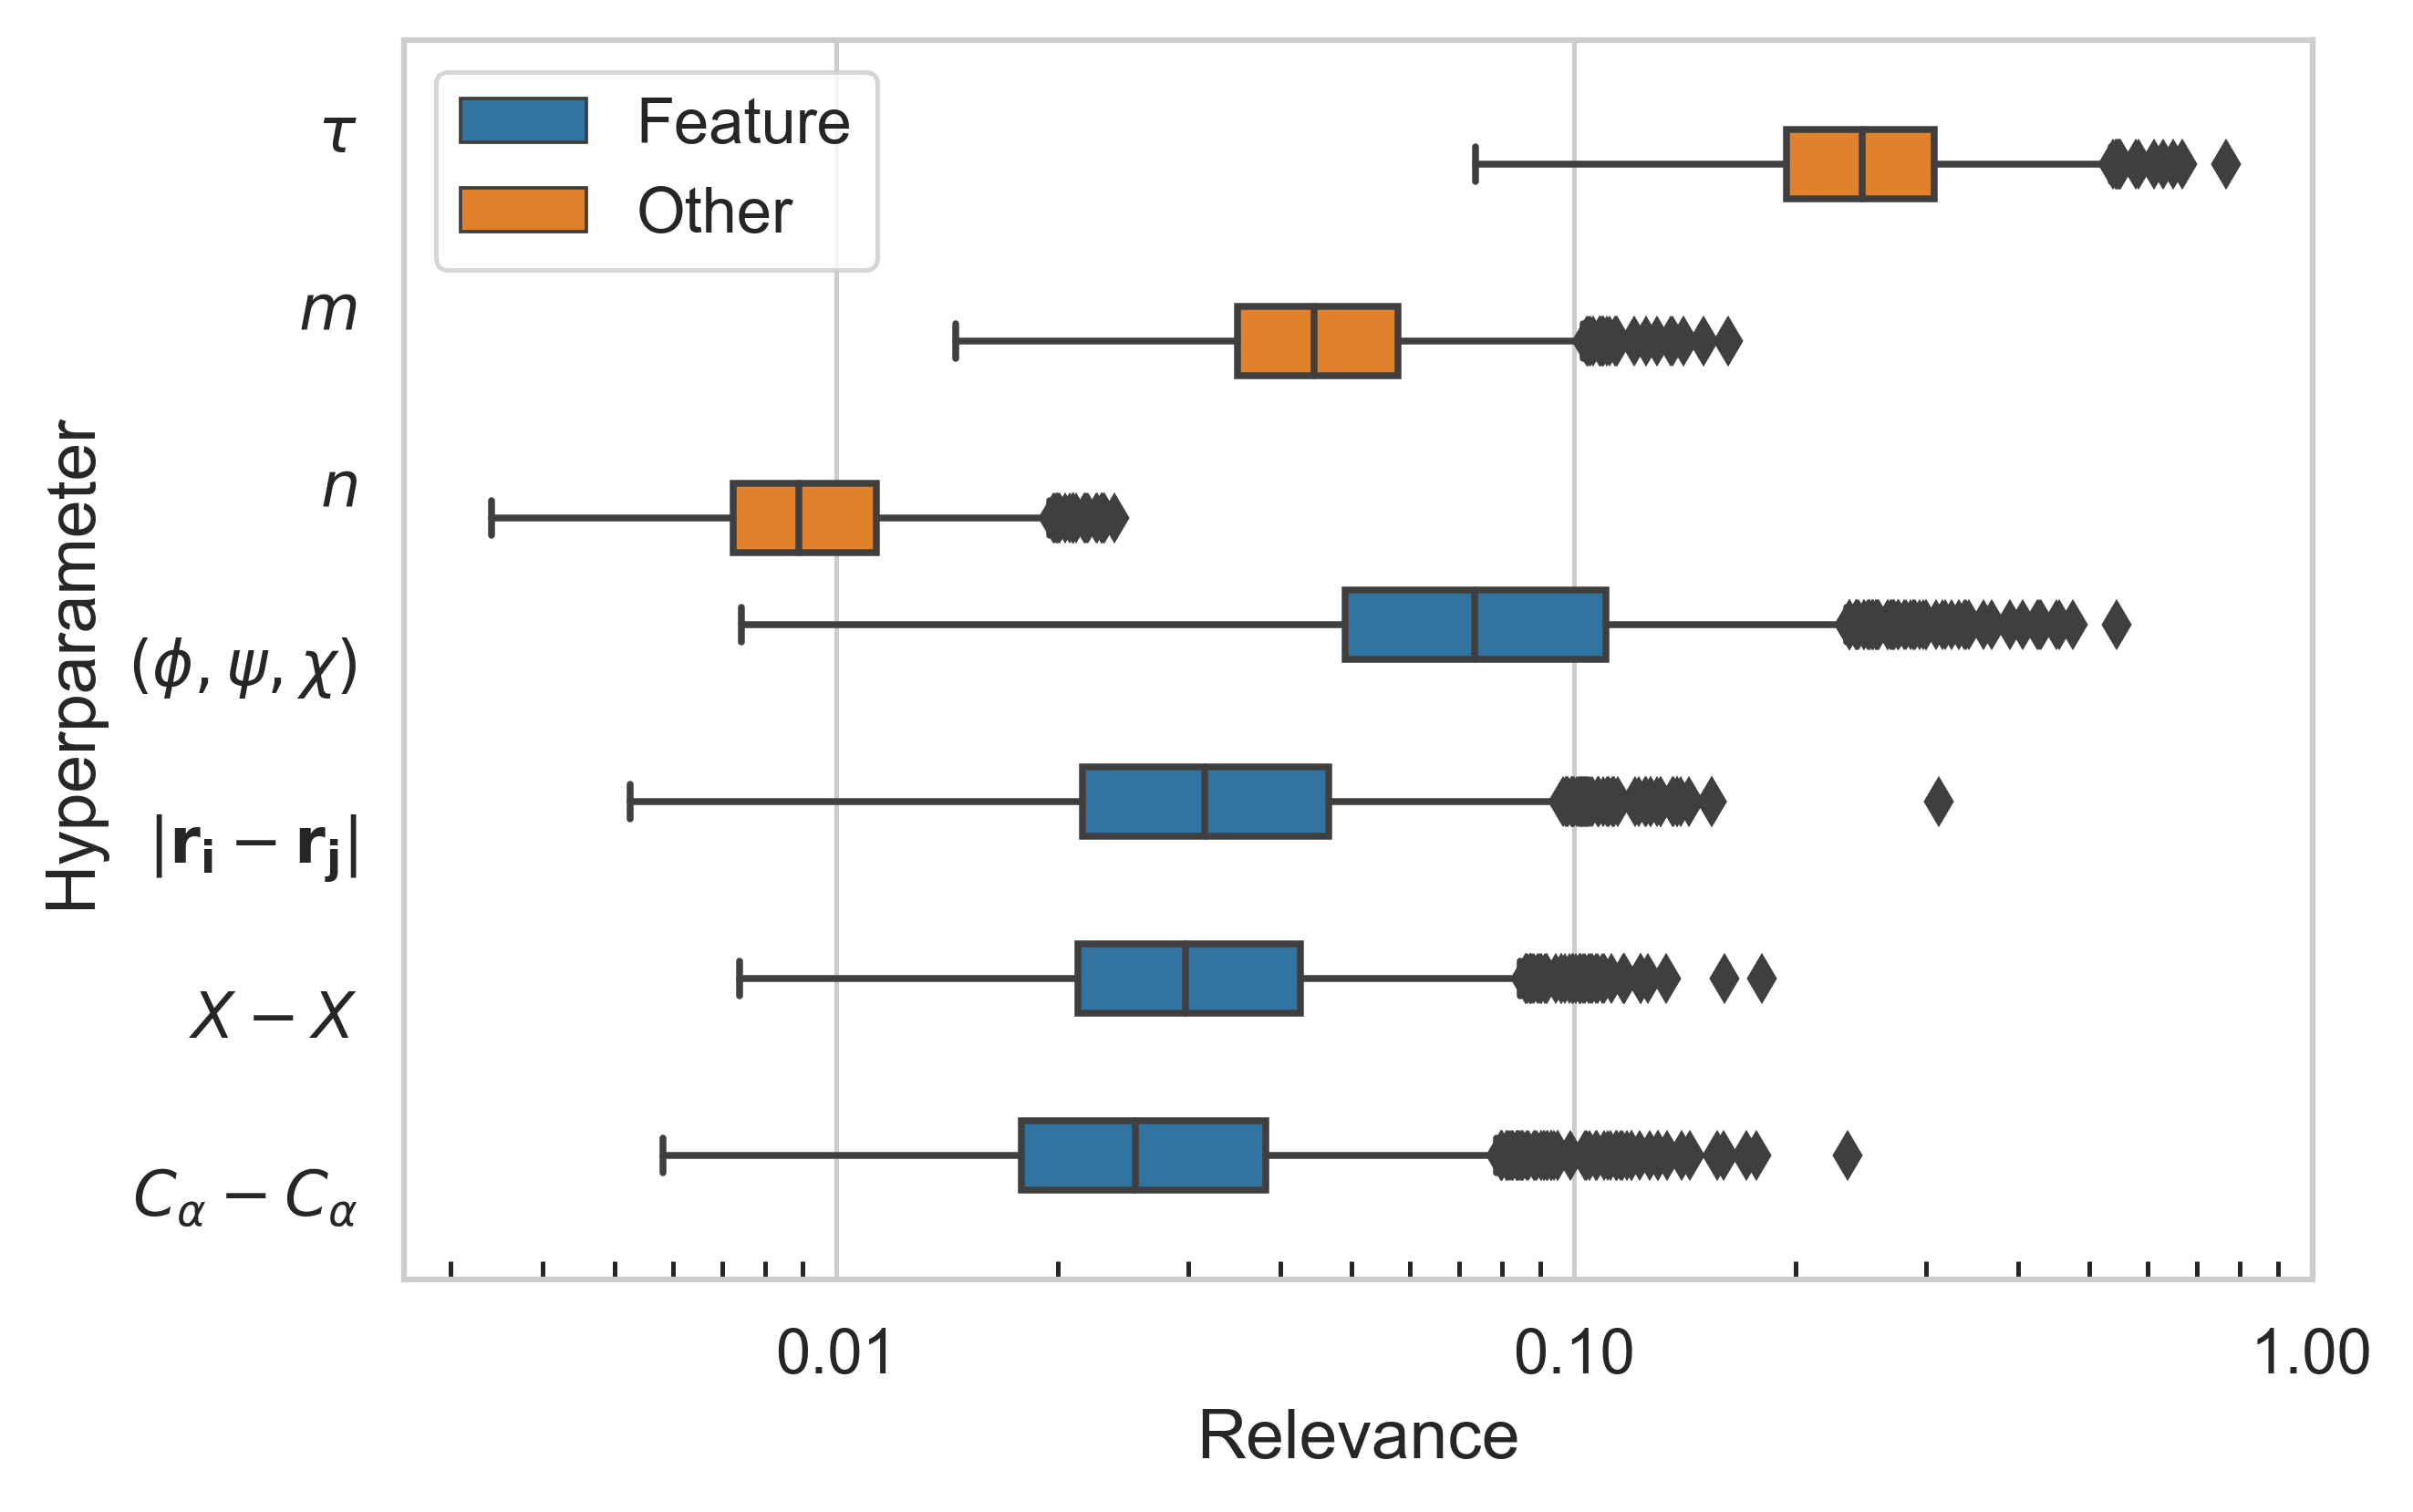
\includegraphics[width=0.8\textwidth]{chapters/msm_optimization/figures/AADH_relevance_d.png}
    \label{fig:aadh_relevance}
\end{figure}

\begin{table}
    \centering
    \mycaption[Posterior distributions of GP parameters]{\textsc{Posterior distributions of GP parameters}. Shown are the median and $\SI{95}{\percent}$ credible intervals for the kernel hyperparameters of the AADH response surface estimated using MCMC with \num{1000} posterior samples. The length-scale parameters in equation \ref{eqn:kernel_form} are re-written here as relevances.}
    \begin{tabular}{|l|r|l|}
    \hline
                             hyperparameter &  Median &     (\SI{95}{\percent}C.I.) \\
    \hline\hline
                    $R_{(\phi, \psi, \chi)}$ &   0.073 &  (0.021-0.248) \\
     $R_{|\mathbf{r_{1}} - \mathbf{r_{2}}|}$ &   0.032 &  (0.012-0.098) \\
                 $R_{C_{\alpha}-C_{\alpha}}$ &   0.025 &  (0.009-0.084) \\
                                   $R_{X-X}$ &   0.030 &  (0.012-0.083) \\
                                  $R_{\tau}$ &   0.246 &  (0.126-0.474) \\
                                     $R_{m}$ &   0.044 &  (0.022-0.095) \\
                                     $R_{n}$ &   0.009 &  (0.005-0.018) \\
                                      $\eta$ &   1.540 &  (1.117-2.154) \\
                                  $\sigma_n$ &   0.011 &  (0.001-0.035) \\
    \hline
    \end{tabular}
    \label{tab:aadh_rel}
\end{table}

The multidimensional nature of the response surface poses problems for visualisation and for understanding the interaction between the hyperparameters in determining the response. However, calculating the hyperparameter relevance can help by suggesting the displayed granularity of the inputs. Figure \ref{fig:aadh_relevance} shows the posterior distribution of relevance for the features (blue) and the remaining hyperparameters (orange). The median and $\SI{95}{\percent}$ credible intervals are tabulated in table \ref{tab:aadh_rel}. 

Figure \ref{fig:aadh_rsm} shows a projection of the response surface, $f(\mathbf{x})$, informed by the relevance. $\tau$ and $m$ are the two highest relevance hyperparameters ($R_{\tau} = \num{0.246}\ [\numrange[range-phrase=-]{0.126}{0.474})]$, $R_{m} = \num{0.044}\ [\numrange[range-phrase=-]{0.022}{0.095}]$) so the response surface is shown as a 2D heat map with $\tau$ on the vertical and $m$ on the horizontal axis. Only odd values of $m$ are shown given the slightly lower relevance of this feature. The number of cluster features is, like the case of alanine dipeptide, the lowest relevance hyperparameter ($R_{n} = \num{0.009}\ [\numrange[range-phrase=-]{0.005}{0.018}]$ and so heat maps for only two value of $n$ are shown: the value at the maximum of the response surface ($n=207$ although the value displayed is rounded to $210$) and $n=1000$. With only four features, it is  simple to show the response surface for each of them. With a larger number of features, displaying the high relevance features and \emph{only one} of the low relevance features would be sufficient. This is because low relevance features are similar.  Note, that this doesn't mean they have a low absolute value but rather that their values are highly correlated. This is clearly borne out with this surface - the two lower relevance features, the contact distances, are very similar and including both in the visualisation is redundant. However, as all features have absolutely low relevance ($R<1$) then their response surfaces are expected to be similar. The maximum of the response surface, shown highlighted with a  white star, occurs at $\mathbf{x}=\left(\chi=(\phi, \psi, \chi), \tau = \SI{12.5}{\nano\second}, m=1, n=207\right)$ with a value of $\mu=\num{3.543 \pm 0.396}$. The features of this response surface will be discussed in the context of sensitivity analysis in section \ref{sec:aadh_sens_analysis}. 

\begin{figure}[p]
    \centering
    \mycaption[The unoptimized response surface of AADH]{\textsc{The unoptimized response surface of AADH, $f\left(\mathbf{x}; \mathcal{D}_{361}\right)$}. For each feature two heat maps are shown with $\tau$ on the vertical axis and $m$ on the horizontal axis. Panel (a) shows the  $(\phi, \psi, \chi)$ feature  with $n=210$,  panel (b) for $n=1000$,  and similarly for the remaining features. The white star denotes the approximate location of the maximum of the surface, the true maximum occurs at $\tau=\SI{12.5}{\nano\second}, m=1, n=207$  The value of the response surface denoted by the color (lighter implies higher values) and with the text annotations.}
    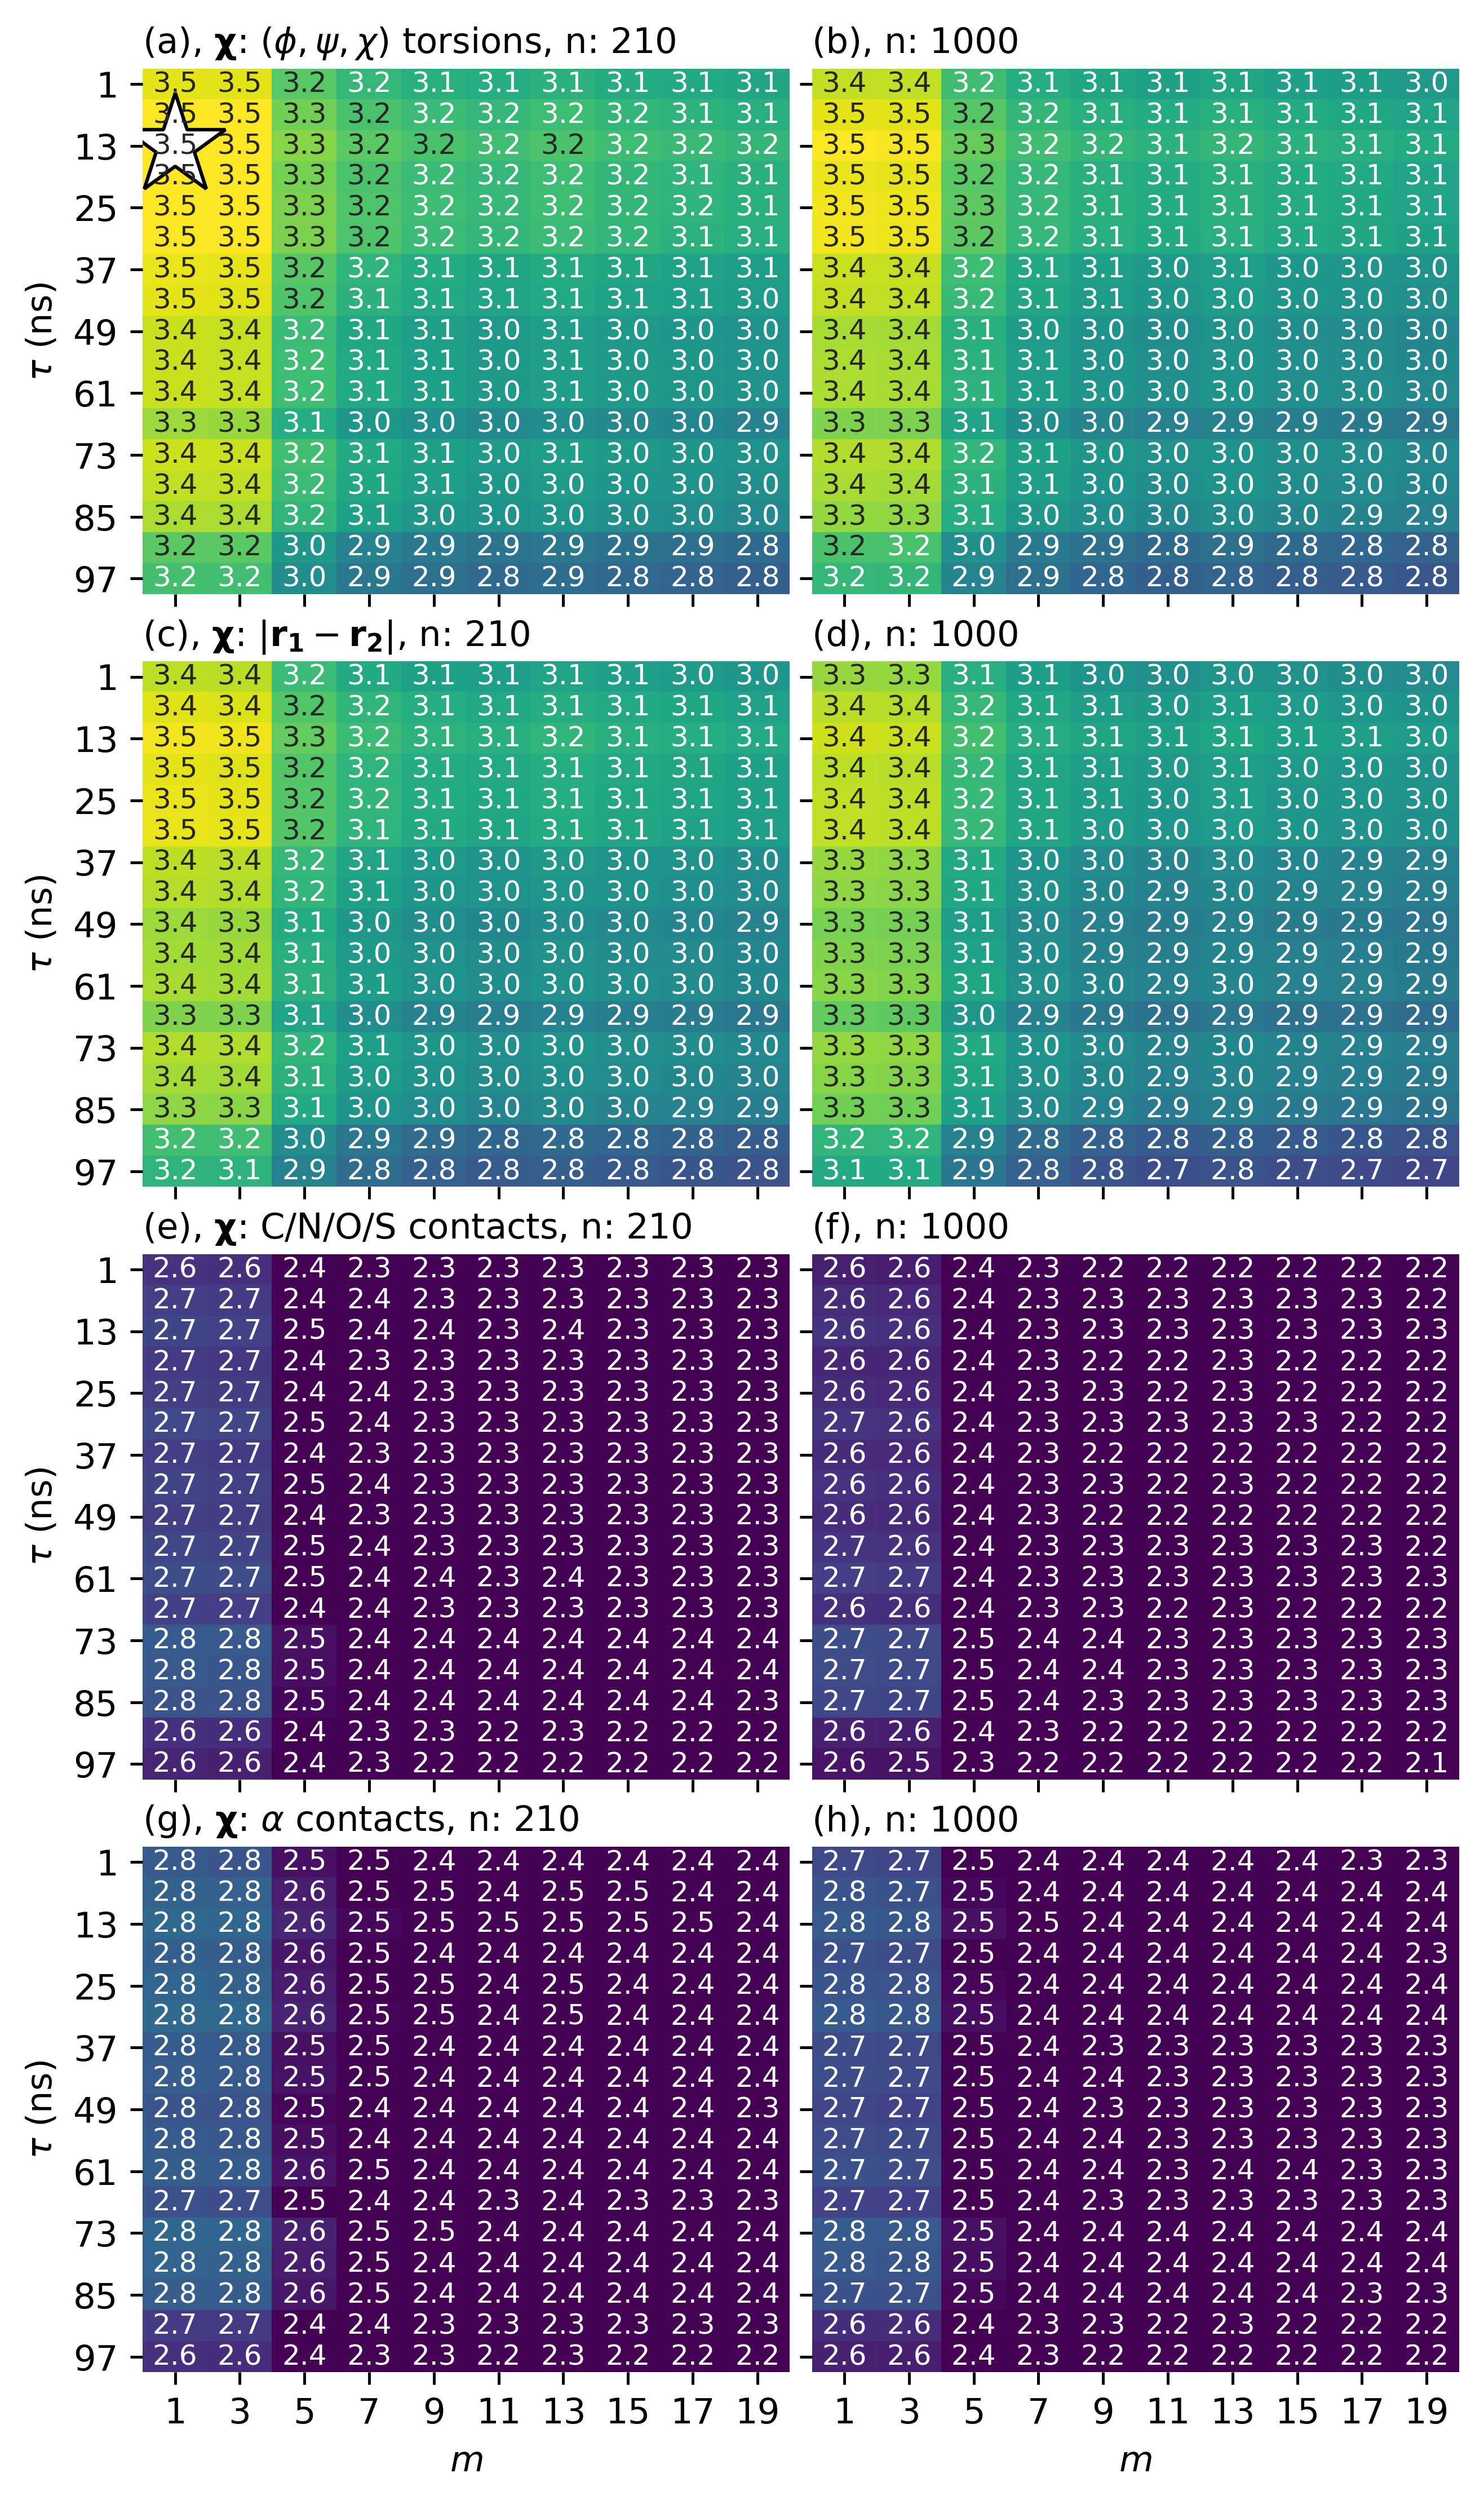
\includegraphics[width=0.7\textwidth]{chapters/msm_optimization/figures/aadh_response_surface_d.png}
    \label{fig:aadh_rsm}
\end{figure}

\subsection{Bayesian optimisation}\label{sec:aadh_bayes_opt}

\begin{table}
    \centering
    \mycaption[MSM hyperparameters pre- and post-Bayesian optimisation]{\textsc{MSM hyperparameters pre- and post-Bayesian optimisation}. Each column represents a Bayesian optimisation experiment, seeded with $N_{\mathrm{seed}}$ randomly sampled hyperparameter trials. Five iterations of optimisation were run with $N_{\mathrm{seed}}=100$ (labelled $\# 1, 2$ etc.) and a single iteration optimising the response surface using all the trial data ($N_{\mathrm{seed}}=361$). Each row is a variable or outcome with values associated with the optimum value of $\mu$ before and after Bayesian optimisation.}
    \begin{tabular}{|ll|lllll|l|}
    \hline
    &$N_{\mathrm{seed}}$ & 100 & & & & &361\\
    &\#&1&2&3&4&5&1\\
    \hline\hline
    $N_{\mathrm{total}}$&Pre&100&100&100&100&100&361\\
    &Post&150&150&150&150&150&410\\
    \hline
    $\mu$&Pre&3.487&3.355&3.599&3.473&3.478&3.543\\
    &Post&3.500&3.558&3.545&3.581&3.569&3.558\\
    \hline
    $\sigma$&Pre&0.152&0.135&0.306&0.234&0.126&0.198\\
    &Post&0.202&0.117&0.101&0.084&0.072&0.091\\
    \hline
    $\chi$&Pre&$(\phi,\psi,\chi)$&$|\mathbf{r_{i}}-\mathbf{r_{j}}|$&$(\phi,\psi,\chi)$&$(\phi,\psi,\chi)$&$|\mathbf{r_{i}}-\mathbf{r_{j}}|$&$(\phi,\psi,\chi)$\\
    &Post&$(\phi,\psi,\chi)$&$(\phi,\psi,\chi)$&$(\phi,\psi,\chi)$&$(\phi,\psi,\chi)$&$(\phi,\psi,\chi)$&$(\phi,\psi,\chi)$\\
    \hline
    $\tau$&Pre&51.0&57.8&12.5&12.5&18.0&12.5\\
    &Post&1.0&4.0&3.0&1.0&1.0&10.0\\
    \hline
    $m$&Pre&1&3&1&1&1&1\\
    &Post&2&1&2&1&1&2\\
    \hline
    $n$&Pre&396&234&207&207&79&207\\
    &Post&10&180&10&230&540&310\\
    \hline
    \end{tabular}
    \label{tab:aadh_opt_results}
\end{table}

% $f(\mathbf{x}; \mathcal{D})$ was then optimized using $50$ iterations of Bayesian optimisation. The final, optimal, set of hyperparameters $\mathbf{x}^{*}\in \mathcal{D}$ were determined as those which maximize the optimized response surface. 

In order to test the convergence of the maximum of $f\left(\mathbf{x}; \mathcal{D}_{361}\right)$, \num{50} steps of Bayesian optimisation was performed. The optimisation was seeded with all the hyperparameter trial observations using the GP model determined in section \ref{sec:aadh_rsm}. At each step of the optimisation, candidate MSM hyperparameters were determined as those which had the highest expected improvement. The grid of points, $\mathbf{X}_{M}$, used to maximize the acquisition function was a $4 \times 100 \times 20 \times 100$ ($\chi \times \tau \times m \times n$) evenly spaced grid. The values of the response and associated hyperparameters pre- and post-optimisation (i.e. $f\left(\mathbf{x}; \mathcal{D}_{361}\right)$ and $f\left(\mathbf{x}; \mathcal{D}_{410}\right)$) are tabulated in the final column of table \ref{tab:aadh_opt_results}. The optimisation resulted in a small improvement in the response from $\mu=3.543 \pm 0.396 \rightarrow 3.558 \pm 0.182$ (a $\SI{0.4}{\percent}$ improvement) with no change in the optimum feature ($(\phi, \psi, \chi)$) and only small changes in the other hyperparameters. The final optimised hyperparameters were: $\chi=(\phi, \psi, \chi), \tau=\SI{10}{\nano\second}, m=2, n=310$. 

In order to see whether this maximum could be reached with a fewer number of trials, five response surfaces fit on random subsets of the trial data with $100$ observations, $f^{i}\left(\mathbf{x};\mathcal{D}_{100}\right),\ i = 1 - 5$, were optimized with \num{50} steps of Bayesian optimisation. The kernel and input warping for $f^{i}\left(\mathbf{x};\mathcal{D}_{100}\right)$ were determined for each $i$ separately. The model selection metrics for each combination of kernel and input warping are tabulated in tables \ref{tab:aadh_rsm_metrics_iter_1} - \ref{tab:aadh_rsm_metrics_iter_5}. The results of the optimisation trials are shown in table \ref{tab:aadh_opt_results} and the incumbent trajectories are shown in are shown in figure \ref{fig:aadh_opt_traj_d}. Also shown, for comparison, in figure \ref{fig:aadh_opt_traj_d} are the maximum of the response surface $f\left(\mathbf{x};\mathcal{D}_{361}\right)$ as orange lines, and the maximum of $f\left(\mathbf{x};\mathcal{D}_{410}\right)$ as blue lines. 

\begin{figure}[p]
    \centering
    \mycaption[Bayesian optimisation trajectories]{\textsc{Bayesian optimisation trajectories}. Each column shows the trajectories of the incumbent $\mu^{*} \pm  2\sigma$ (panels (a) - (e)), and the accompanying value of: $\chi$ (panels (f) - (j)), $m$ (panels (k) - (o)), $\tau$ (panels (p) - (t)) and $n$ (panels (u) - (y)). The location of the final value of the trajectory is highlighted with a black star. For reference the corresponding values determined from the response surface using all the hyperparameter trials are shown as solid horizontal lines: the response surface before optimisation ( $f\left(\mathbf{x}; \mathcal{D}_{361}\right)$) are shown in orange and after Bayesian optimisation ( $f\left(\mathbf{x}; \mathcal{D}_{410}\right)$) in blue.}
    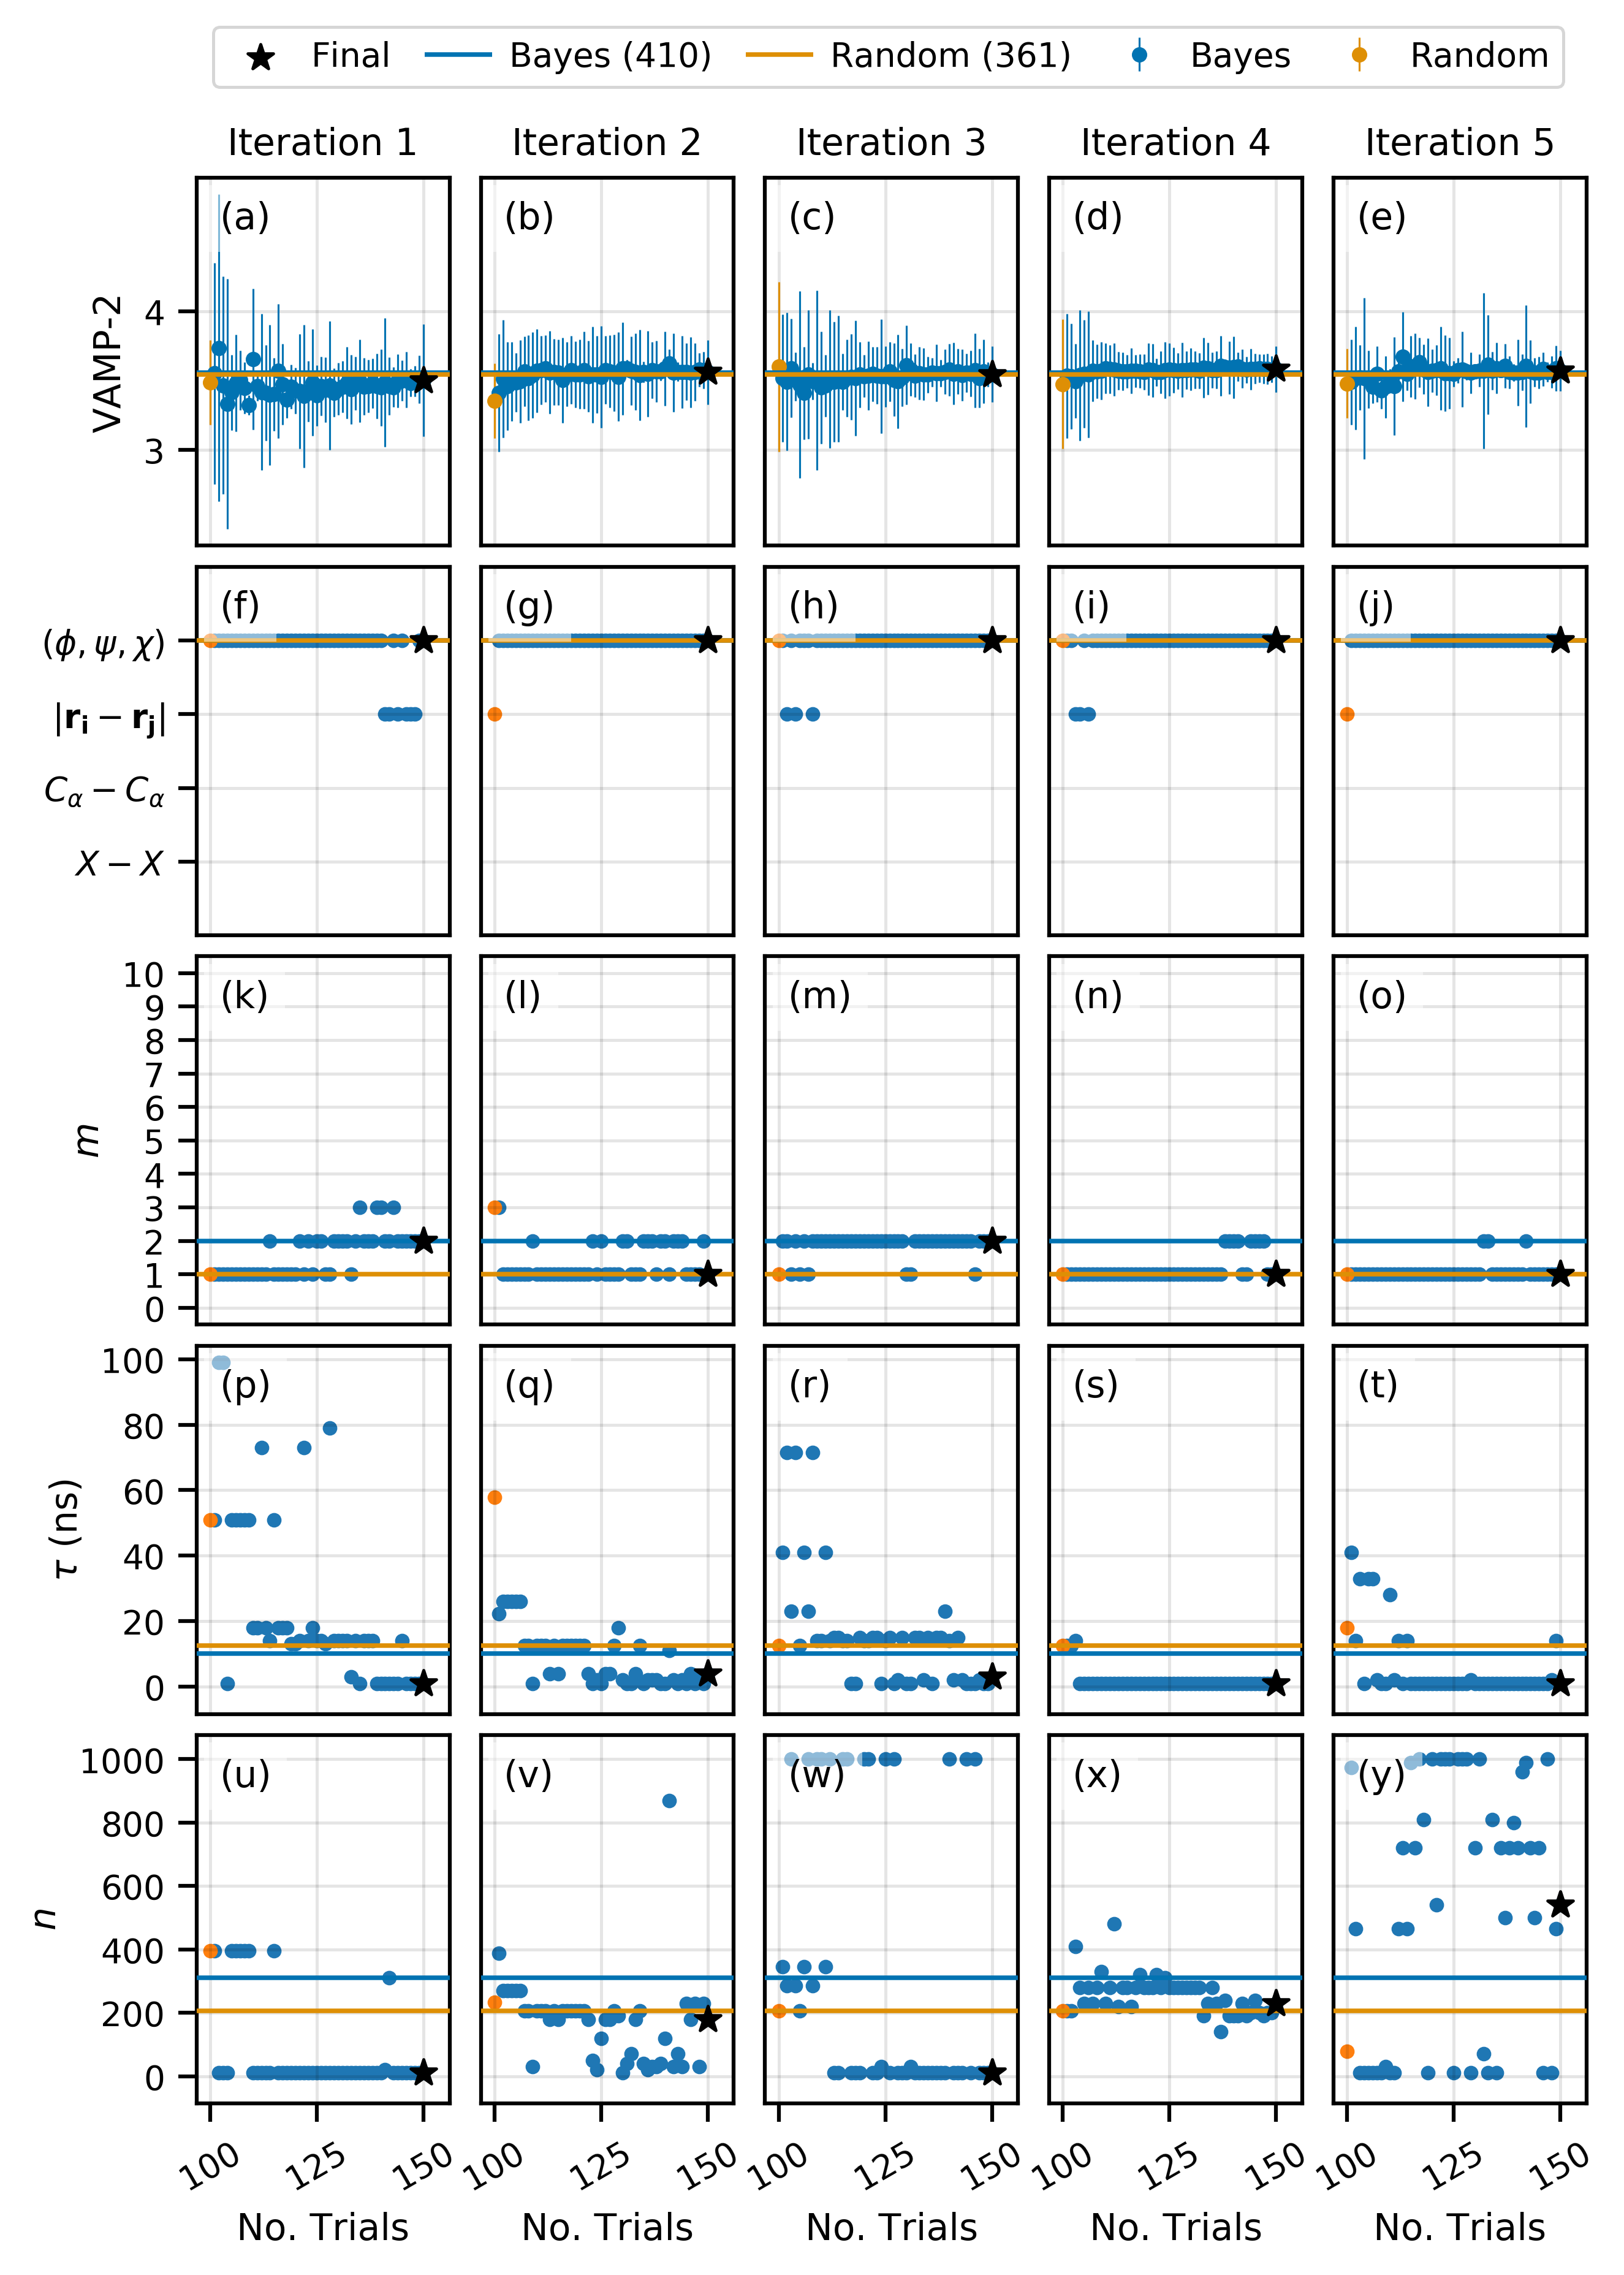
\includegraphics[width=0.8\textwidth]{chapters/msm_optimization/figures/aadh_opt_traj_act_s_d.png}
    \label{fig:aadh_opt_traj_d}
\end{figure}

From  table \ref{tab:aadh_opt_results} it can be seen that after Bayesian optimisation each subset had maxima indistinguishable from the maxima after seeding with the full data set $f\left(\mathbf{x};\mathcal{D}_{461}\right)$: each had the same optimal feature ($(\phi, \psi, \chi)$ dihedral angles), slightly smaller values of $\tau$ (\SIrange{1}{4}{\nano\second} cf. \SI{10}{\nano\second}), similar values of $m$ ($\numrange{1}{2}$ cf. $2$) but with a range of different values of $n$ ($\numrange{10}{540}$ cf. $310$). The extent to which these differences to make a difference the final MSM and its interpretation will be discussed in section \ref{sec:aadh_sens_analysis} in the context of the sensitivity analyses.

It is clear that Bayesian optimisation only had a small effect on the value of the incumbent and on the optimum hyperparameters.  The value of incumbent throughout the procedure (figure \ref{fig:aadh_opt_traj_d} panels (a) - (e)) remained relatively constant. The largest increase came from iteration $4$, with $\Delta \mu 0.108$ and there was even a slight decrease in iteration $3$ with $\Delta \mu = -0.054$ although when including the uncertainty they were statistically indistinguishable from each other. The optimisation procedure also had negligible effects on the value of $\chi$, $m$ and $n$. It did however explore large values of  $\tau$ before settling on its final optimum value in most of the iterations.

The optimisation procedure did not strongly increase the incumbent of each iteration, i.e.,  $f^{i}(\mathbf{x};\mathcal{D}_{150})-f^{i}(\mathbf{x};\mathcal{D}_{100})$ was small. However, the maxima and optimum hyperparameters of the optimized response surfaces $f^{i}\left(\mathbf{x};\mathcal{D}_{150}\right)$ are almost indistinguishable from $f\left(\mathbf{x};\mathcal{D}_{461}\right)$. This suggests that the Bayesian optimisation procedure could be seeded with fewer than \num{100} trials if a GP model of the response surface could be estimated reliably. 

\subsection{Sensitivity analysis}\label{sec:aadh_sens_analysis}

\begin{figure}
    \centering
    \mycaption[Implied timescales of the base case MSM]{\textsc{Implied timescales of the base case MSM}. Timescales were estimated using MCMC with \num{500} posterior samples. Panel (a) shows the implied timescales for $\tau(\mathrm{MSM}) = \SIrange[range-phrase=-]{0.1}{5}{\nano\second}$  and panel (b) for $\tau(\mathrm{MSM}) = \SIrange[range-phrase=-]{0.1}{50}{\nano\second}$. The solid lines are the mean of the posteriors, the shaded areas are the  \SI{95}{\percent} credible intervals. The grey shaded area is the region for which the implied timescales are smaller than $\tau(\mathrm{MSM})$.}\label{fig:aadh_its}
    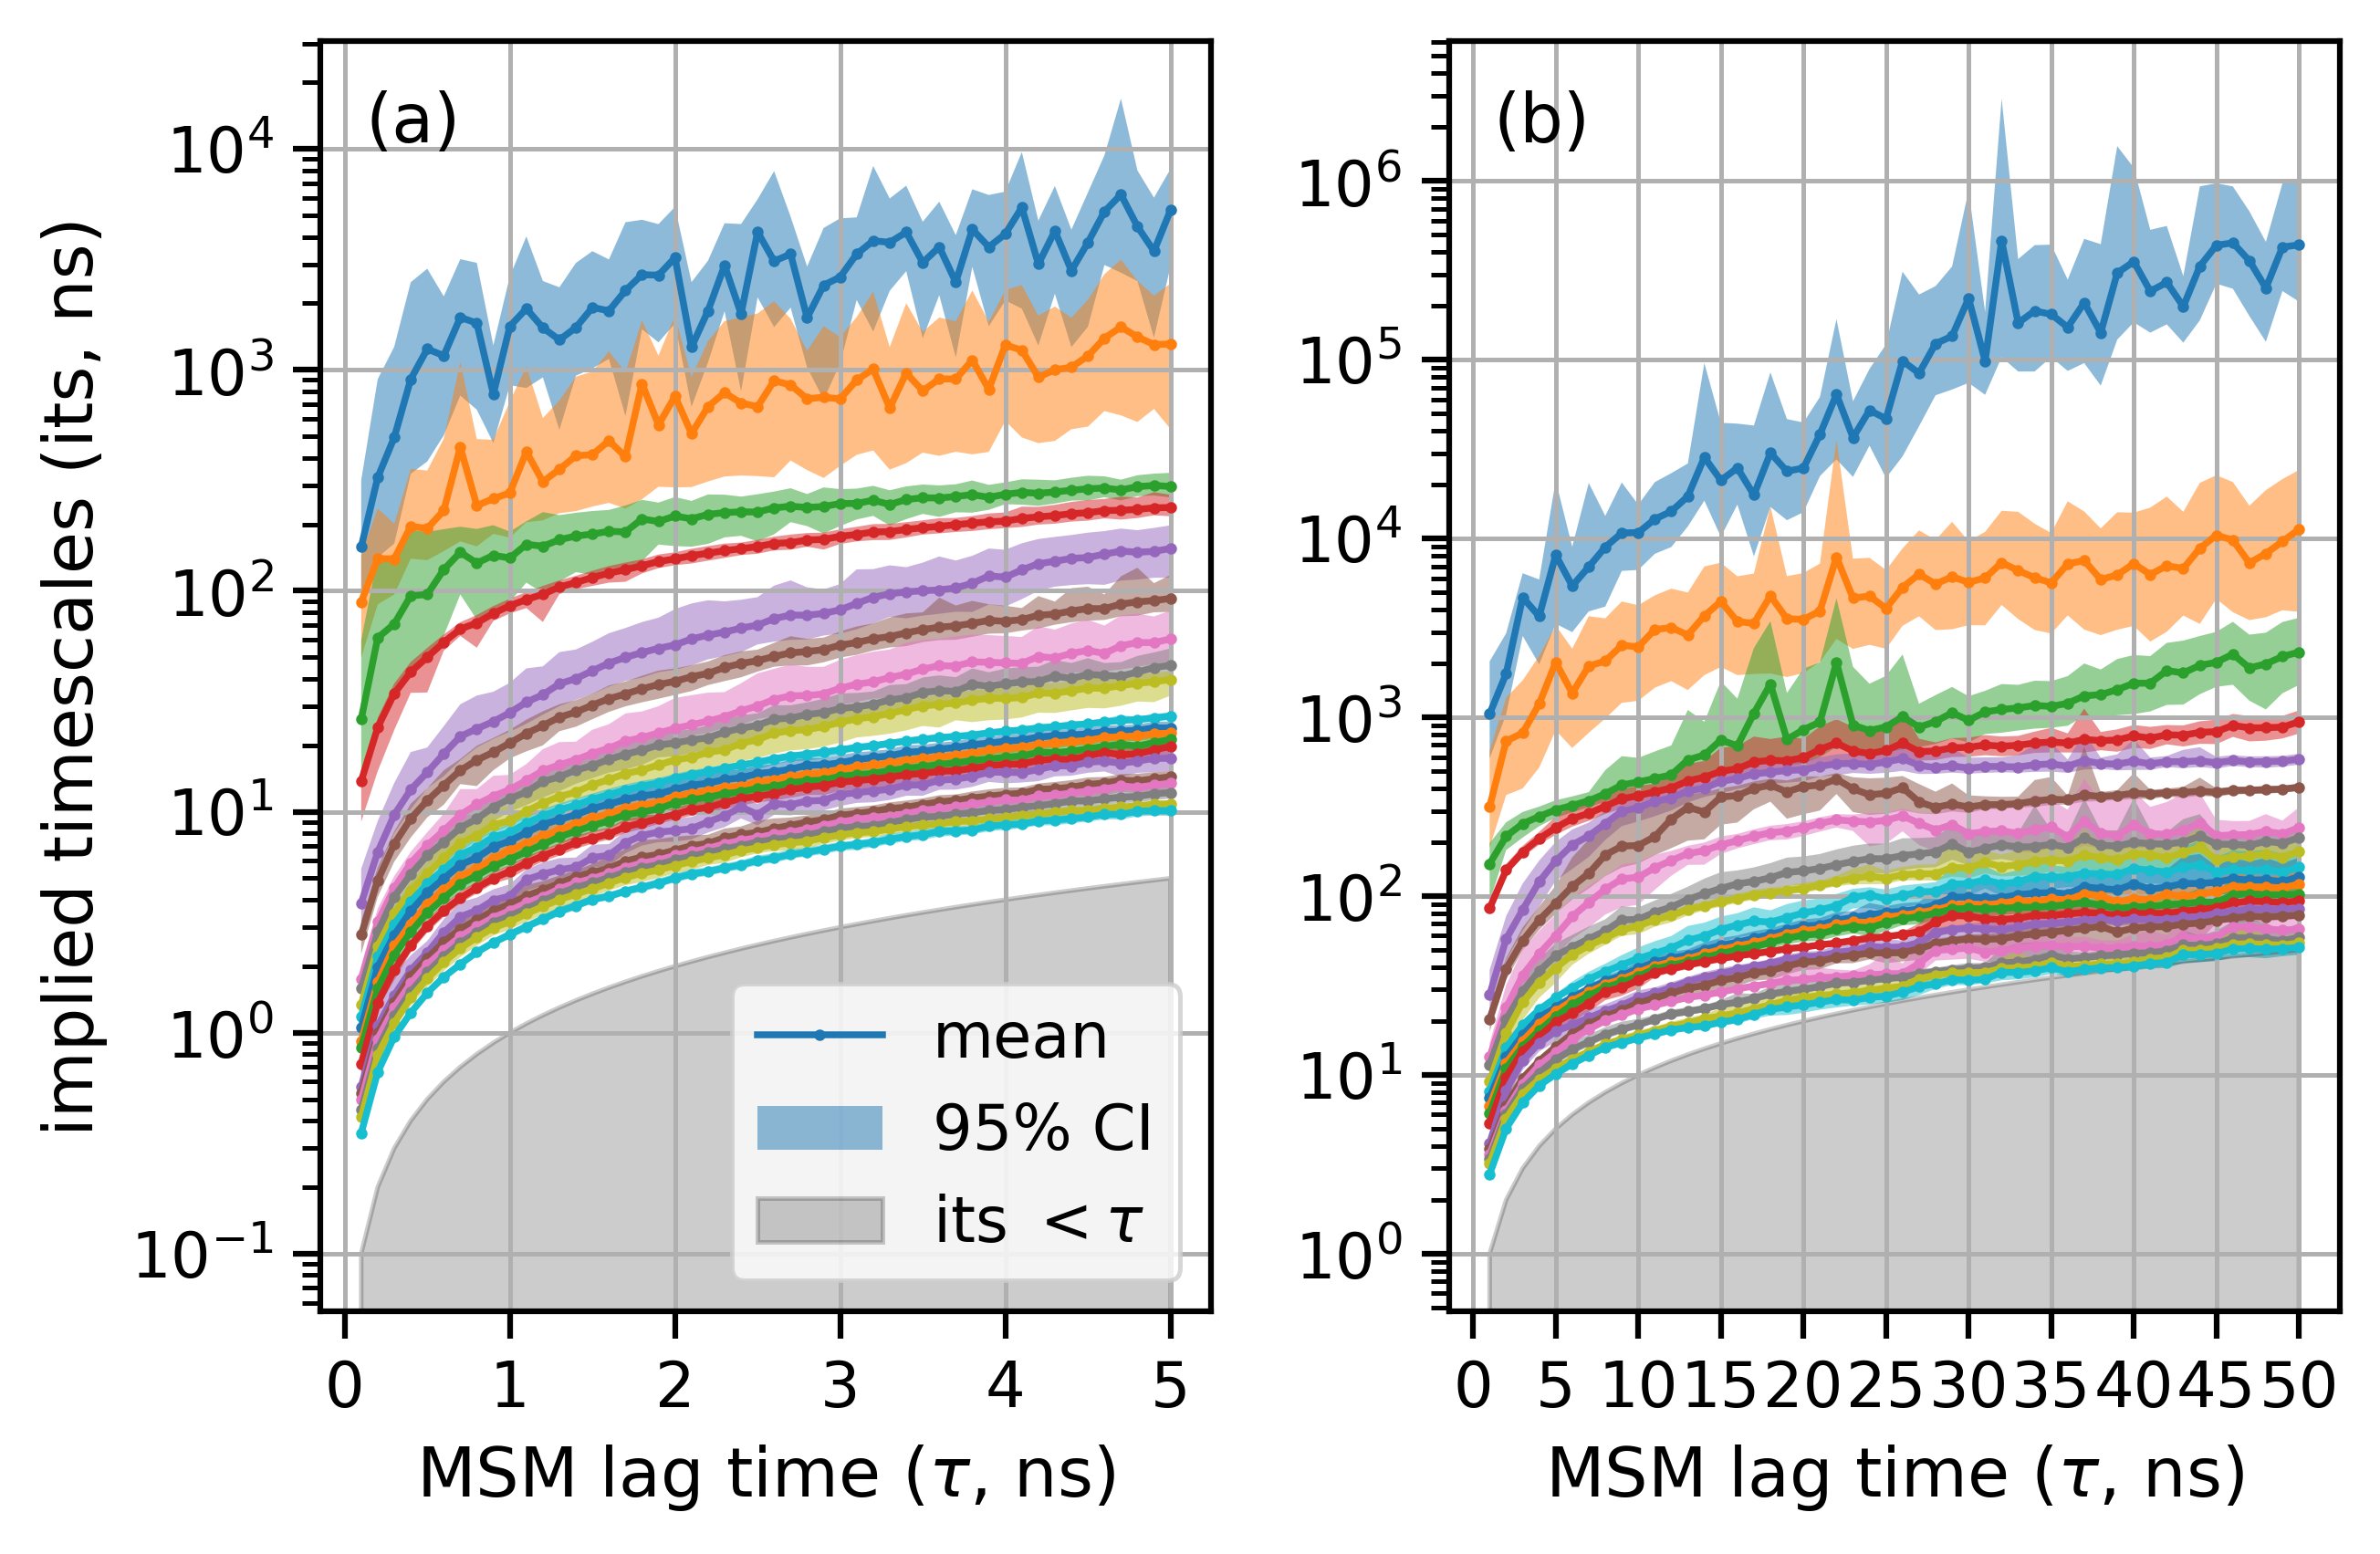
\includegraphics[width=0.8\linewidth]{chapters/msm_optimization/figures/aadh_implied_timescales.png}
\end{figure}

So far the response surface for AADH has been modelled and optimised with a combination of random hyperparameter sampling and Bayesian optimisation under two assumptions about the model specification: that $\tau(\mathrm{MSM}) = \SI{2}{\nano\second}$ and $r=4$ are reasonable assumptions about the lag time and number of slow relaxation processes. As these were established on the basis of the reference MSM it is important to test these assumptions are still reasonable with the final optimized MSM. 

To test the suitability of $\tau(\mathrm{MSM})$ the implied timescales of a series of MSMs fit with the optimum hyperparameters but different lag times are shown in figure \ref{fig:aadh_its}. Panel (a) shows shows the implied timescales for $\tau(\mathrm{MSM}) = \SIrange[range-phrase=-]{0.1}{5}{\nano\second}$ which clearly shows there is a slight increase in the top two implied timescales ($t_{2}$ and $t_{3}$ suggesting that $\tau(\mathrm{MSM})$ may be too small. Looking at the implied timescales over a larger range, $\tau(\mathrm{MSM}) = \SIrange[range-phrase=-]{0.1}{50}{\nano\second}$ (panel (b)), shows that there is a small plateau in $t_{2}$ and $t_{3}$  around  \SIrange{15}{20}{\nano\second}. It is therefore not possible on this evidence alone to say definitively whether $\tau(\mathrm{MSM})$ should be $2$ or $\SI{20}{\nano\second}$ or whether it makes a difference to non-quantitative aspects of the final model.  

At $\tau = \SI{2}{\nano\second}$ there is no clear separation of timescales between the first four relaxation processes (taking into account the uncertainty in $t_{2}$ and $t_{3}$), however there is a gap between $t_{5}$ and $t_{6}$ suggesting $r=5$ would be more appropriate than the $r=4$ previously chosen. This means the fourth relaxation process ($t_{5}$, shown in red in figure \ref{fig:aadh_its}) has not been factored into the response. In principle this means that there may be different hyperparameters which maximize VAMP-2, however given the similarity between $t_{4}$ and $t_{5}$ this may not be very plausible or significant, if true. At $\tau(\mathrm{MSM}) = \SI{20}{\nano\second}$ there is a clear separation between $t_{2}$ and $t_{3}$ suggesting $r=2$ is appropriate. In this case we have included potentially too many fast processes. While changing the value of $r$ will certainly change the value of the optimal hyperparameters, given the mixed evidence in the eigenvalue spectrum there is no reason to reject this optimized MSM. The associated question of how many metastable states and dominant relaxation processes actually matter for explaining the observed data will be investigated in section \ref{sec:aadh_hmm}. 

Knowledge of the response surface and of the eigenvalue spectrum suggests sensitivity analyses to understand the validity and robustness of the optimum MSM.  The goal of sensitivity analyses is to have faith that reasonable changes in model choices and hyperparameters do not materially affect inferences from the model. Typically we are concerned with inferring relaxation timescales ($t_{i}$), the character of the relaxation process ($\Psi_{i}$) and the lumping of the microstates into metastable states. The VAMP-2 score has served as a proxy for the quality of the inferences required from the model but this is not sufficient  for a number of reasons.  First, in general it may be sensitive to both the MSM lag time and the number of eigenfunctions used in the definition. Second, as figure \ref{fig:ala1_evcompare} has demonstrated, VAMP-2 is not sensitive to the discretisation error. This is also evident in the fact that in both iteration $1$ and $3$ (table \ref{tab:aadh_opt_results}) the optimal value of $n=10$ with only a very small difference in response at these values $\mu = 3.500$ and   $\mu=3.545$ cf. $\mu=3.558$). Third, the phenomenon of the Rashomon effect\cite{breiman2001} in statistical modelling, where  multiple \emph{different} statistical models result in the performance metric, could be at play here.

The standard validation check of MSMs, the Chapman-Kolmogorov test (section \ref{sec:model_validation}), relies on coarse graining transition matrix, which will be discussed in section \ref{sec:aadh_hmm}. The current discussion will center on the eigenvalue spectrum and qualitative aspects of the free energy surface and eigenfunctions. For the optimal MSM (hereafter labelled `base case'), these are all shown in figure \ref{fig:aadh_msm_best}: panels (a) - (c) show the eigenvectors of the first three relaxation processes ($\Psi_{2} - \Psi_{4}$) in the space of the first two TICA components. Panel (d) shows the implied timescales for the first $10$ relaxation processes (coloured according to whether they were included in the VAMP-2 score), and panel (e) shows the free energy surface in the space of the first two TICA components.

\begin{figure}
    \centering
    \mycaption[The optimised response surface of AADH]{\textsc{The optimised response surface of AADH, $f\left(\mathbf{x}; \mathcal{D}_{410}\right)$}. The response surface was estimated using both the randomly sampled and optimised hyperparameters. For each feature a single heat map are shown for $n=310$, with $\tau$ on the vertical axis and $m$ on the horizontal axis. All values of $m$ in the range $1\le m \le 10$ are shown. The white star denotes the approximate location of the maximum of the surface, the true maximum occurs at $\tau=\SI{10}{\nano\second}, m=2, n=310$. The value of the response surface is denoted by the color (lighter implies higher values) and with the text annotations.}
    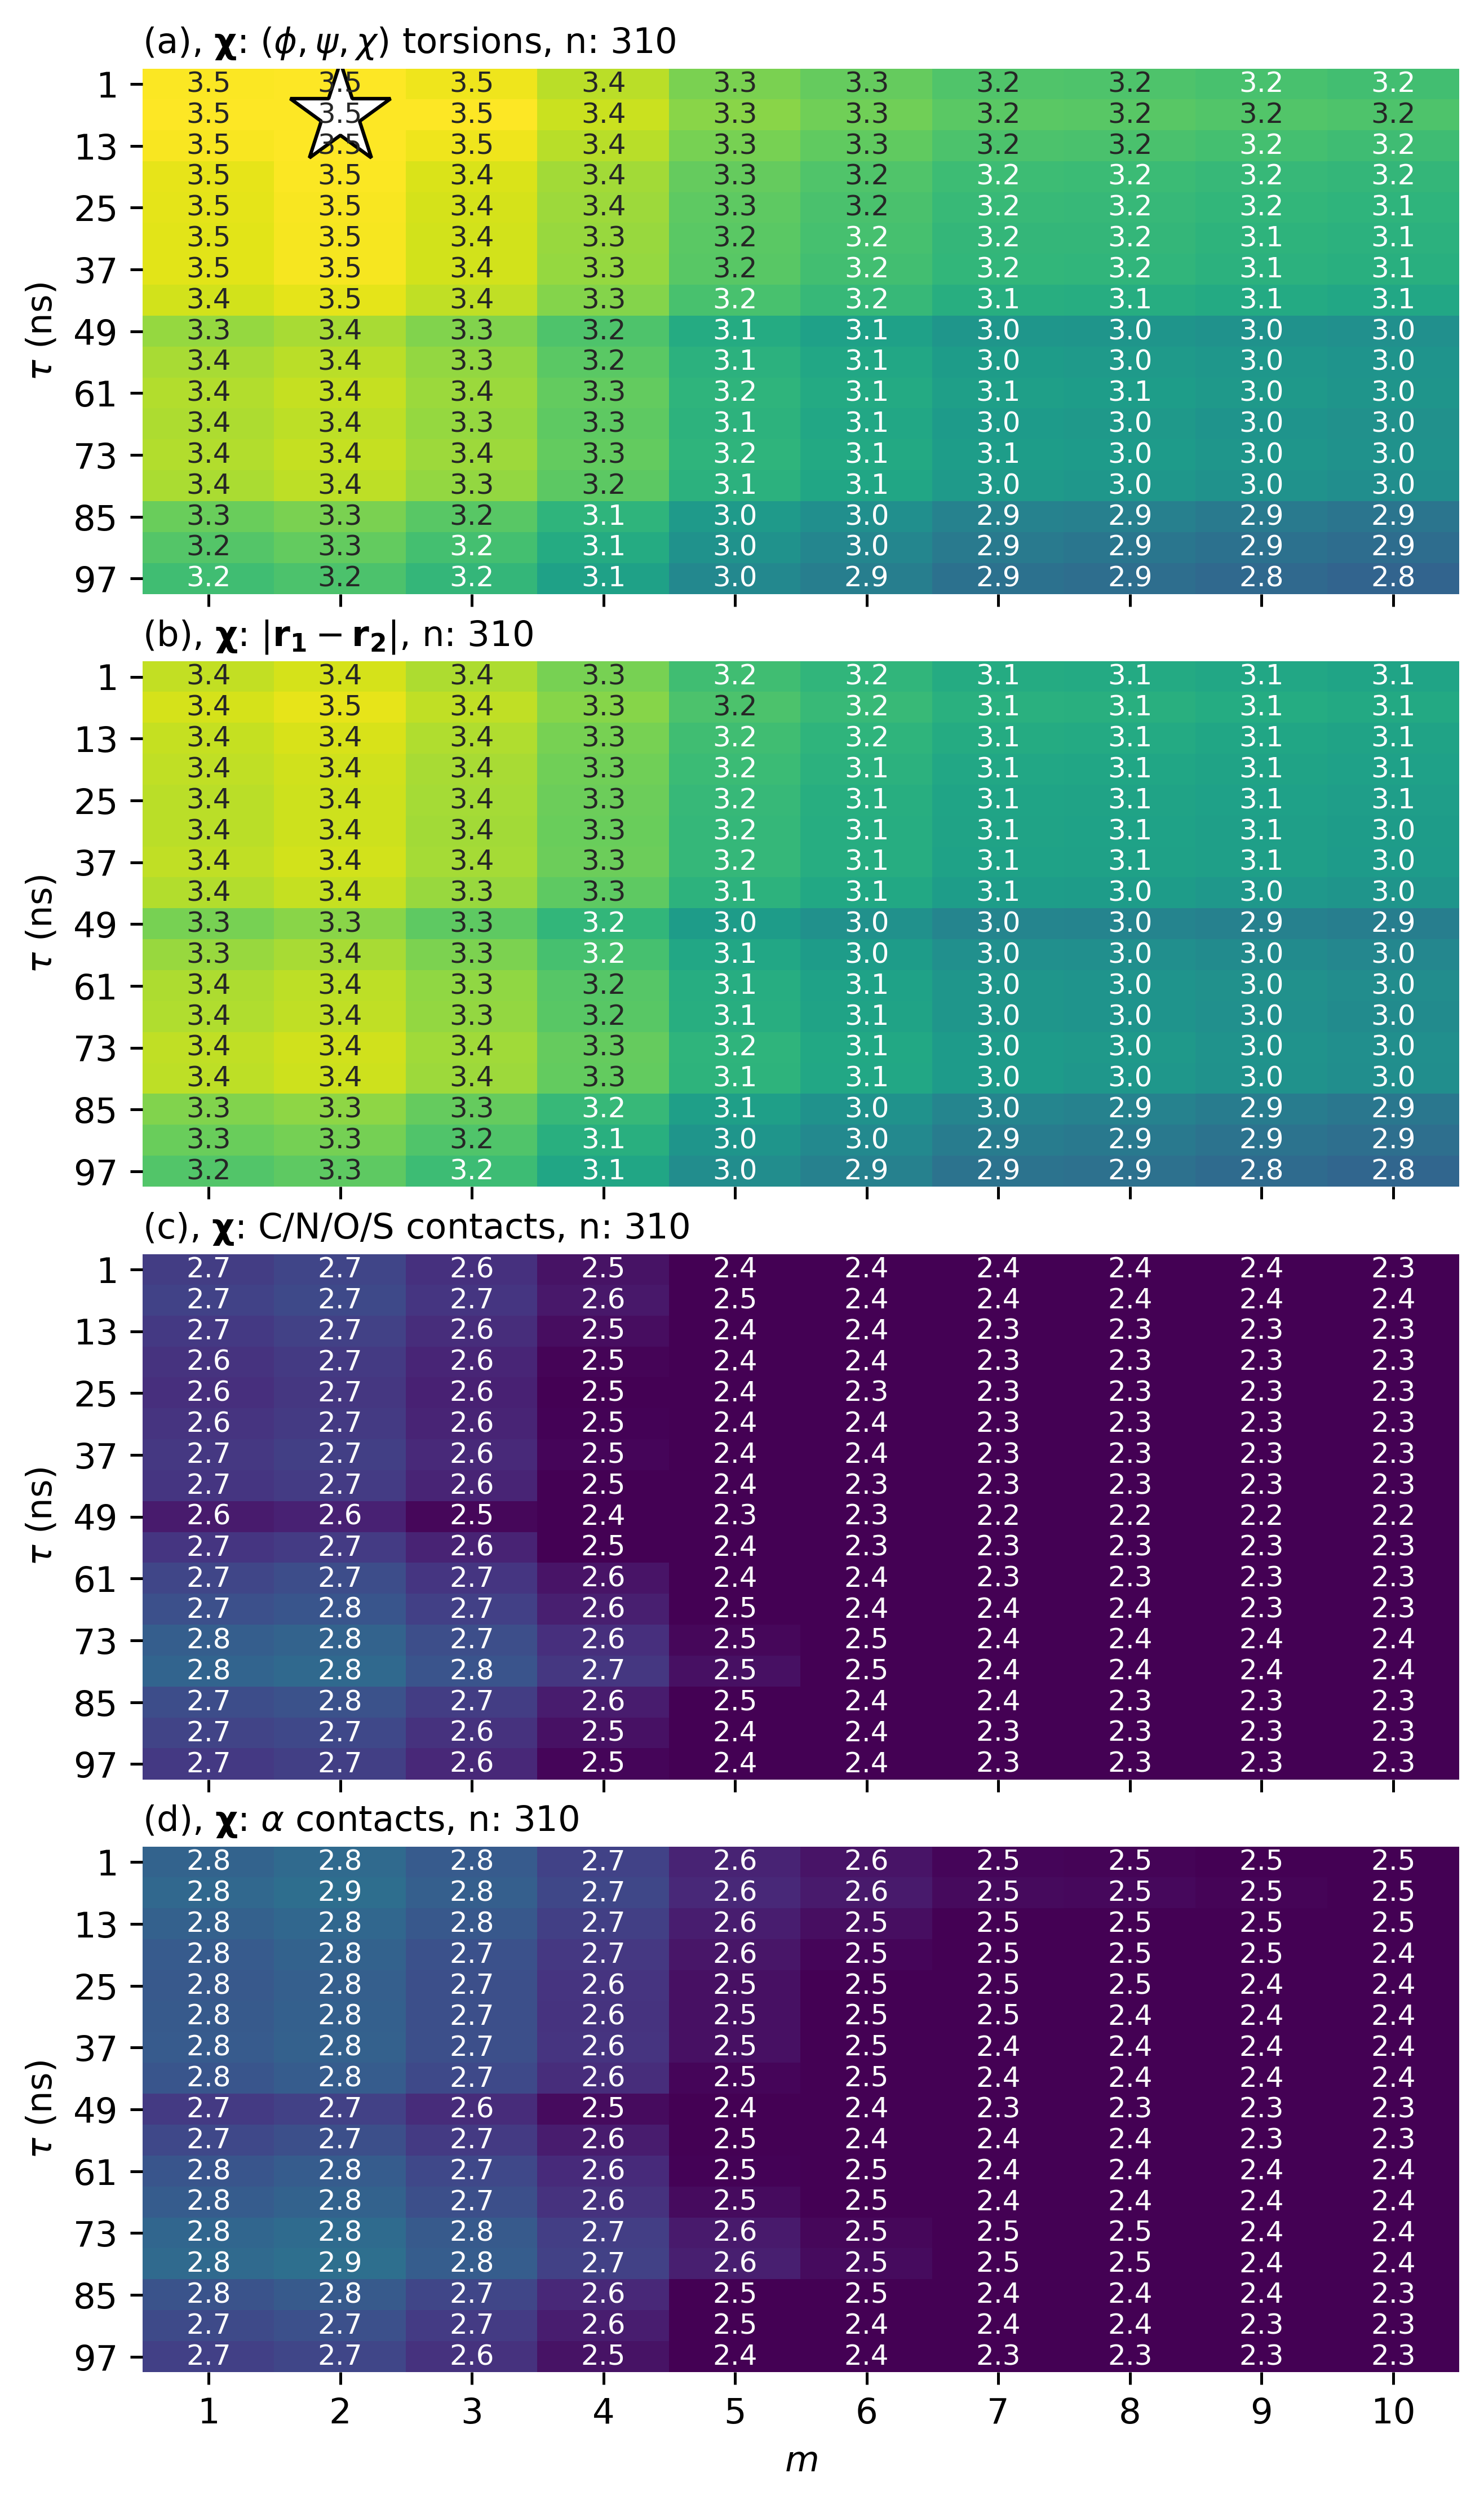
\includegraphics[width=0.6\textwidth]{chapters/msm_optimization/figures/aadh_response_surface_d_opt.png.png}
    \label{fig:aadh_rsm_opt}
\end{figure}


\begin{figure}
    \centering
    \mycaption[Base case MSM]{\textsc{Base case MSM}. The MSM was estimated with the optimum hyperparameters: $\chi= (\phi, \psi, \chi)$, $\tau=\SI{10}{\nano\second}$, $m=2$ and $n=310$. Panels (a), (b) and (c) show the non-trivial eigenvectors used in the VAMP-2 score, the horizontal and vertical axes are the first two TICA components. Panel (d) are the first ten implied timescales, colored according to whether they were used in the VAMP-2 score. The error bars are the $\SI{95}{\percent}$ credible intervals.  Panel (e) is the free energy with the same axes as panels (a) - (c). The MSM was estimated using MCMC with \num{1000} posterior samples.}
    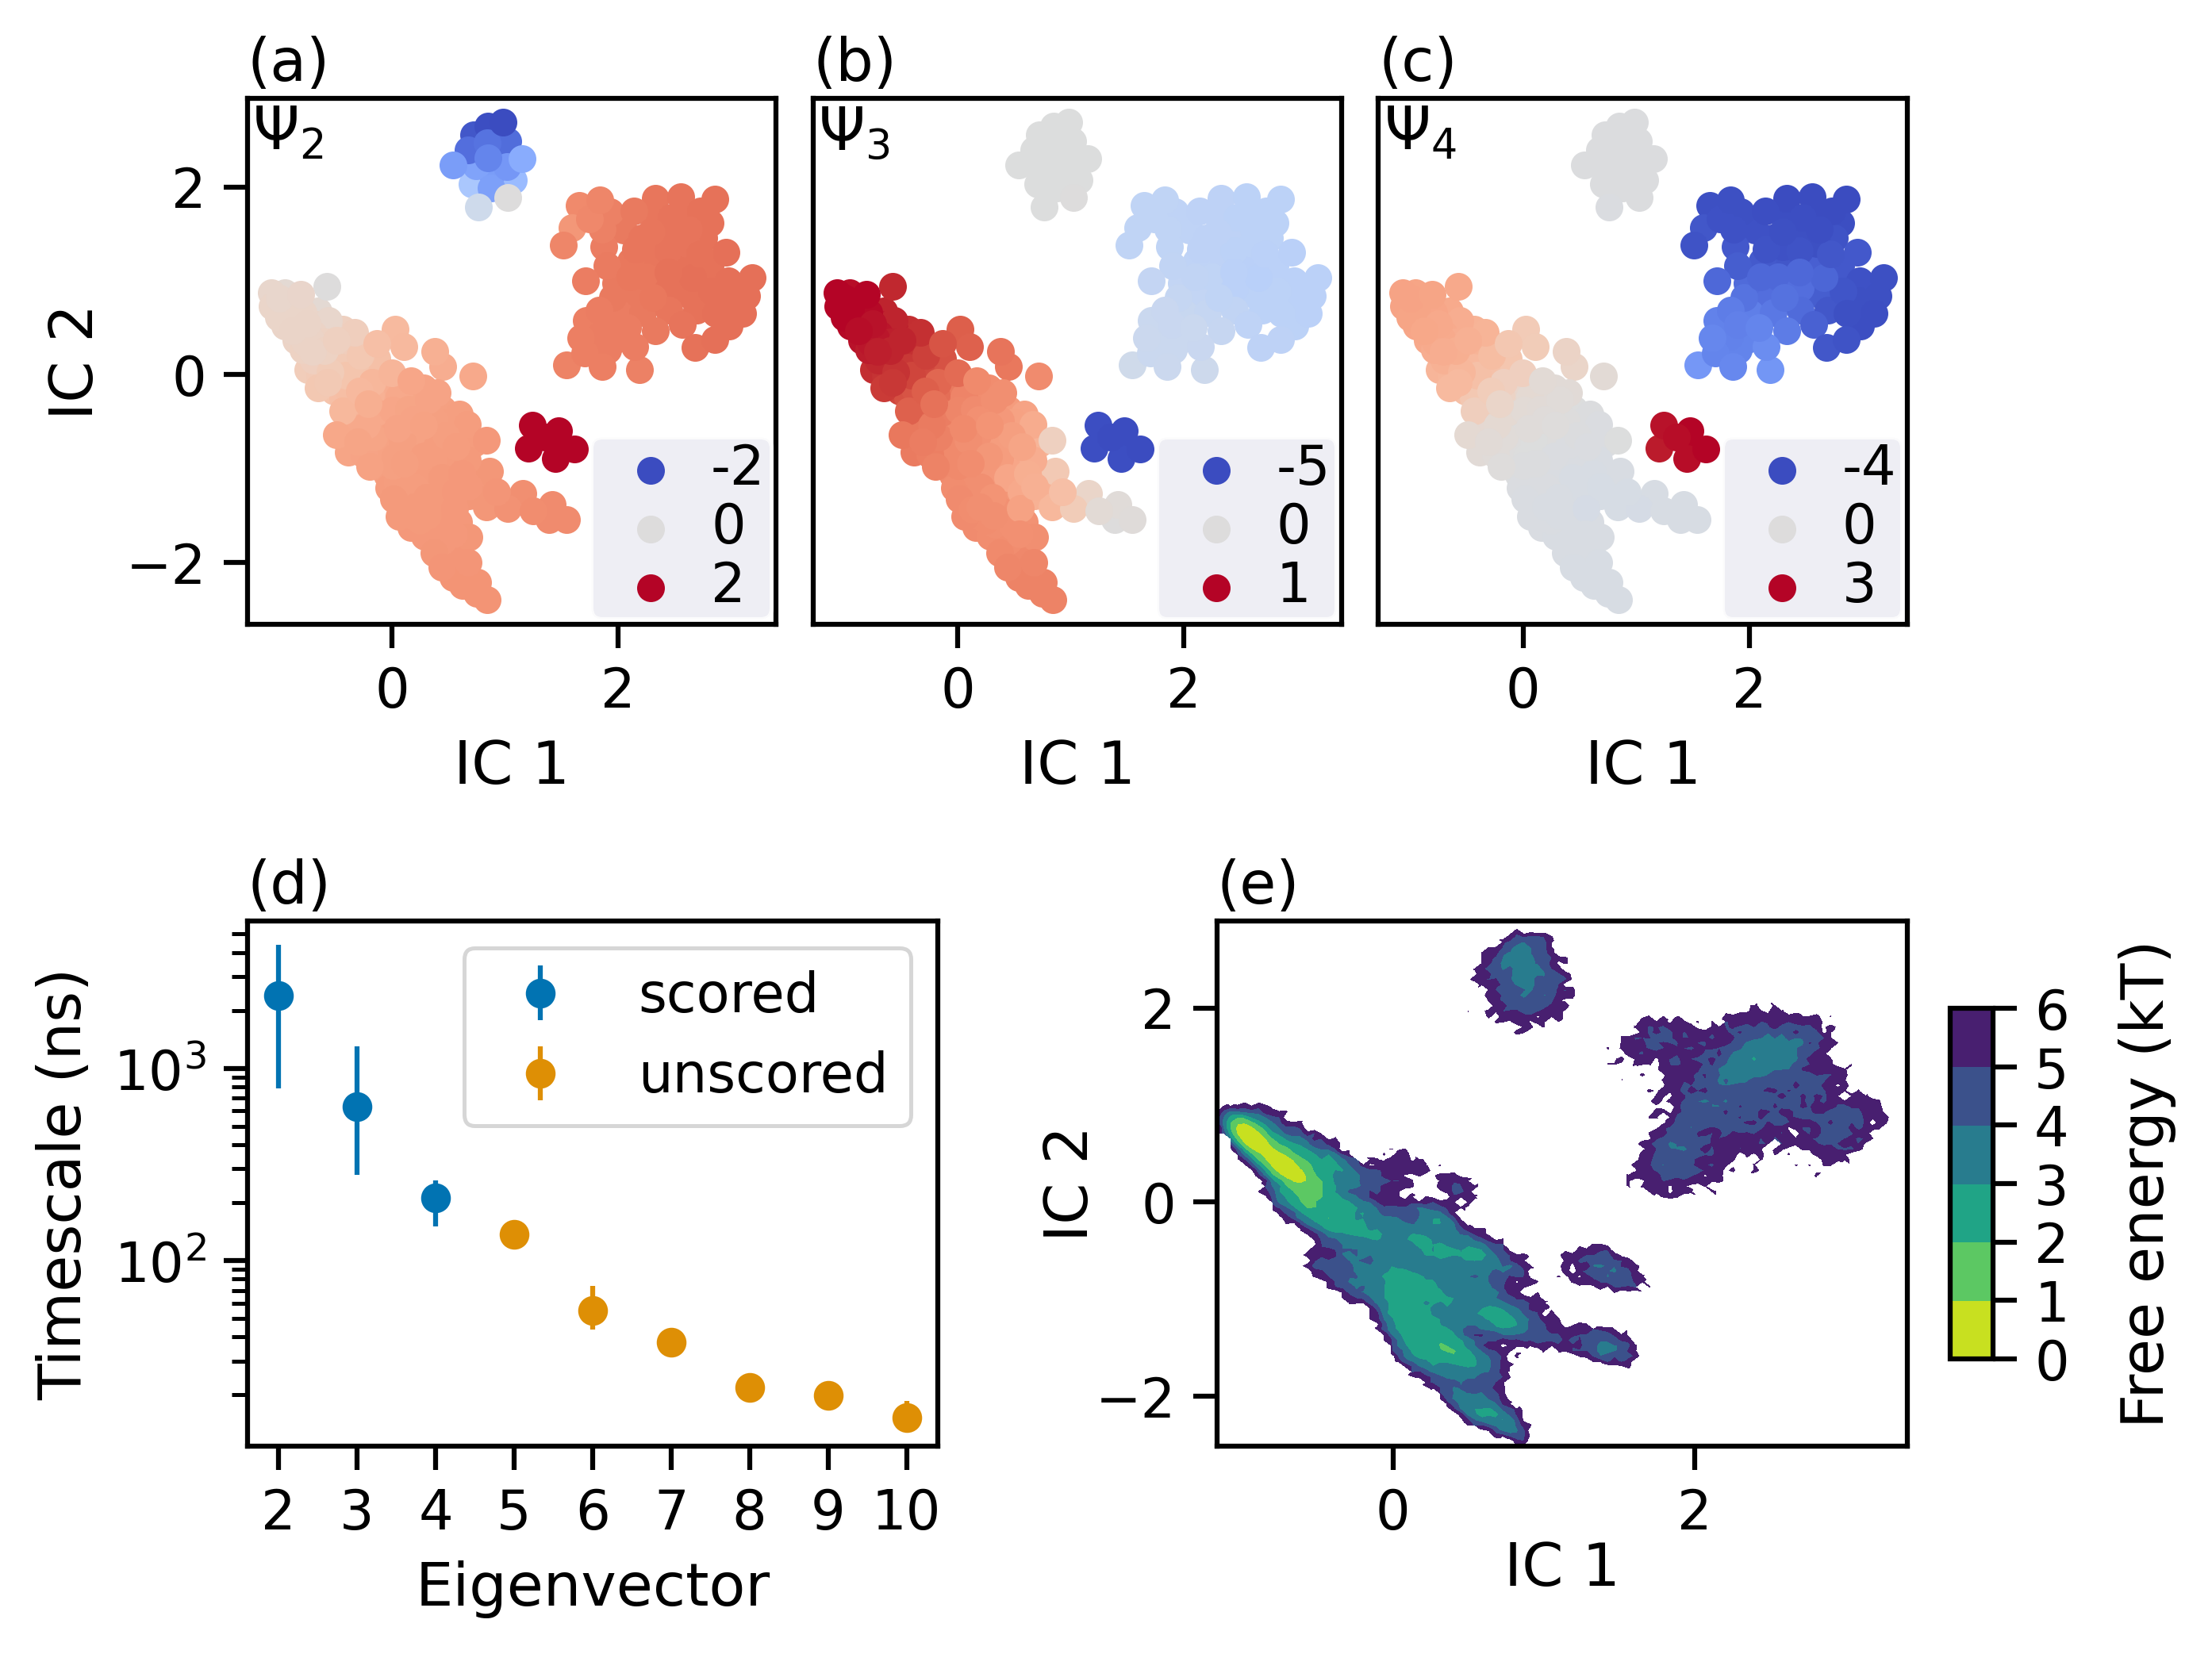
\includegraphics[width=0.8\textwidth]{chapters/msm_optimization/figures/aadh_msm_best.png}
    \label{fig:aadh_msm_best}
\end{figure}

\begin{figure}
    \centering
    \mycaption[Sensitivity 1 MSM]{\textsc{Sensitivity 1 MSM}. The MSM has the same hyperparameters as the base case but with $\tau(\mathrm{MSM})=\SI{20}{\nano\second}$. See caption of figure \ref{fig:aadh_msm_best} for details.}
    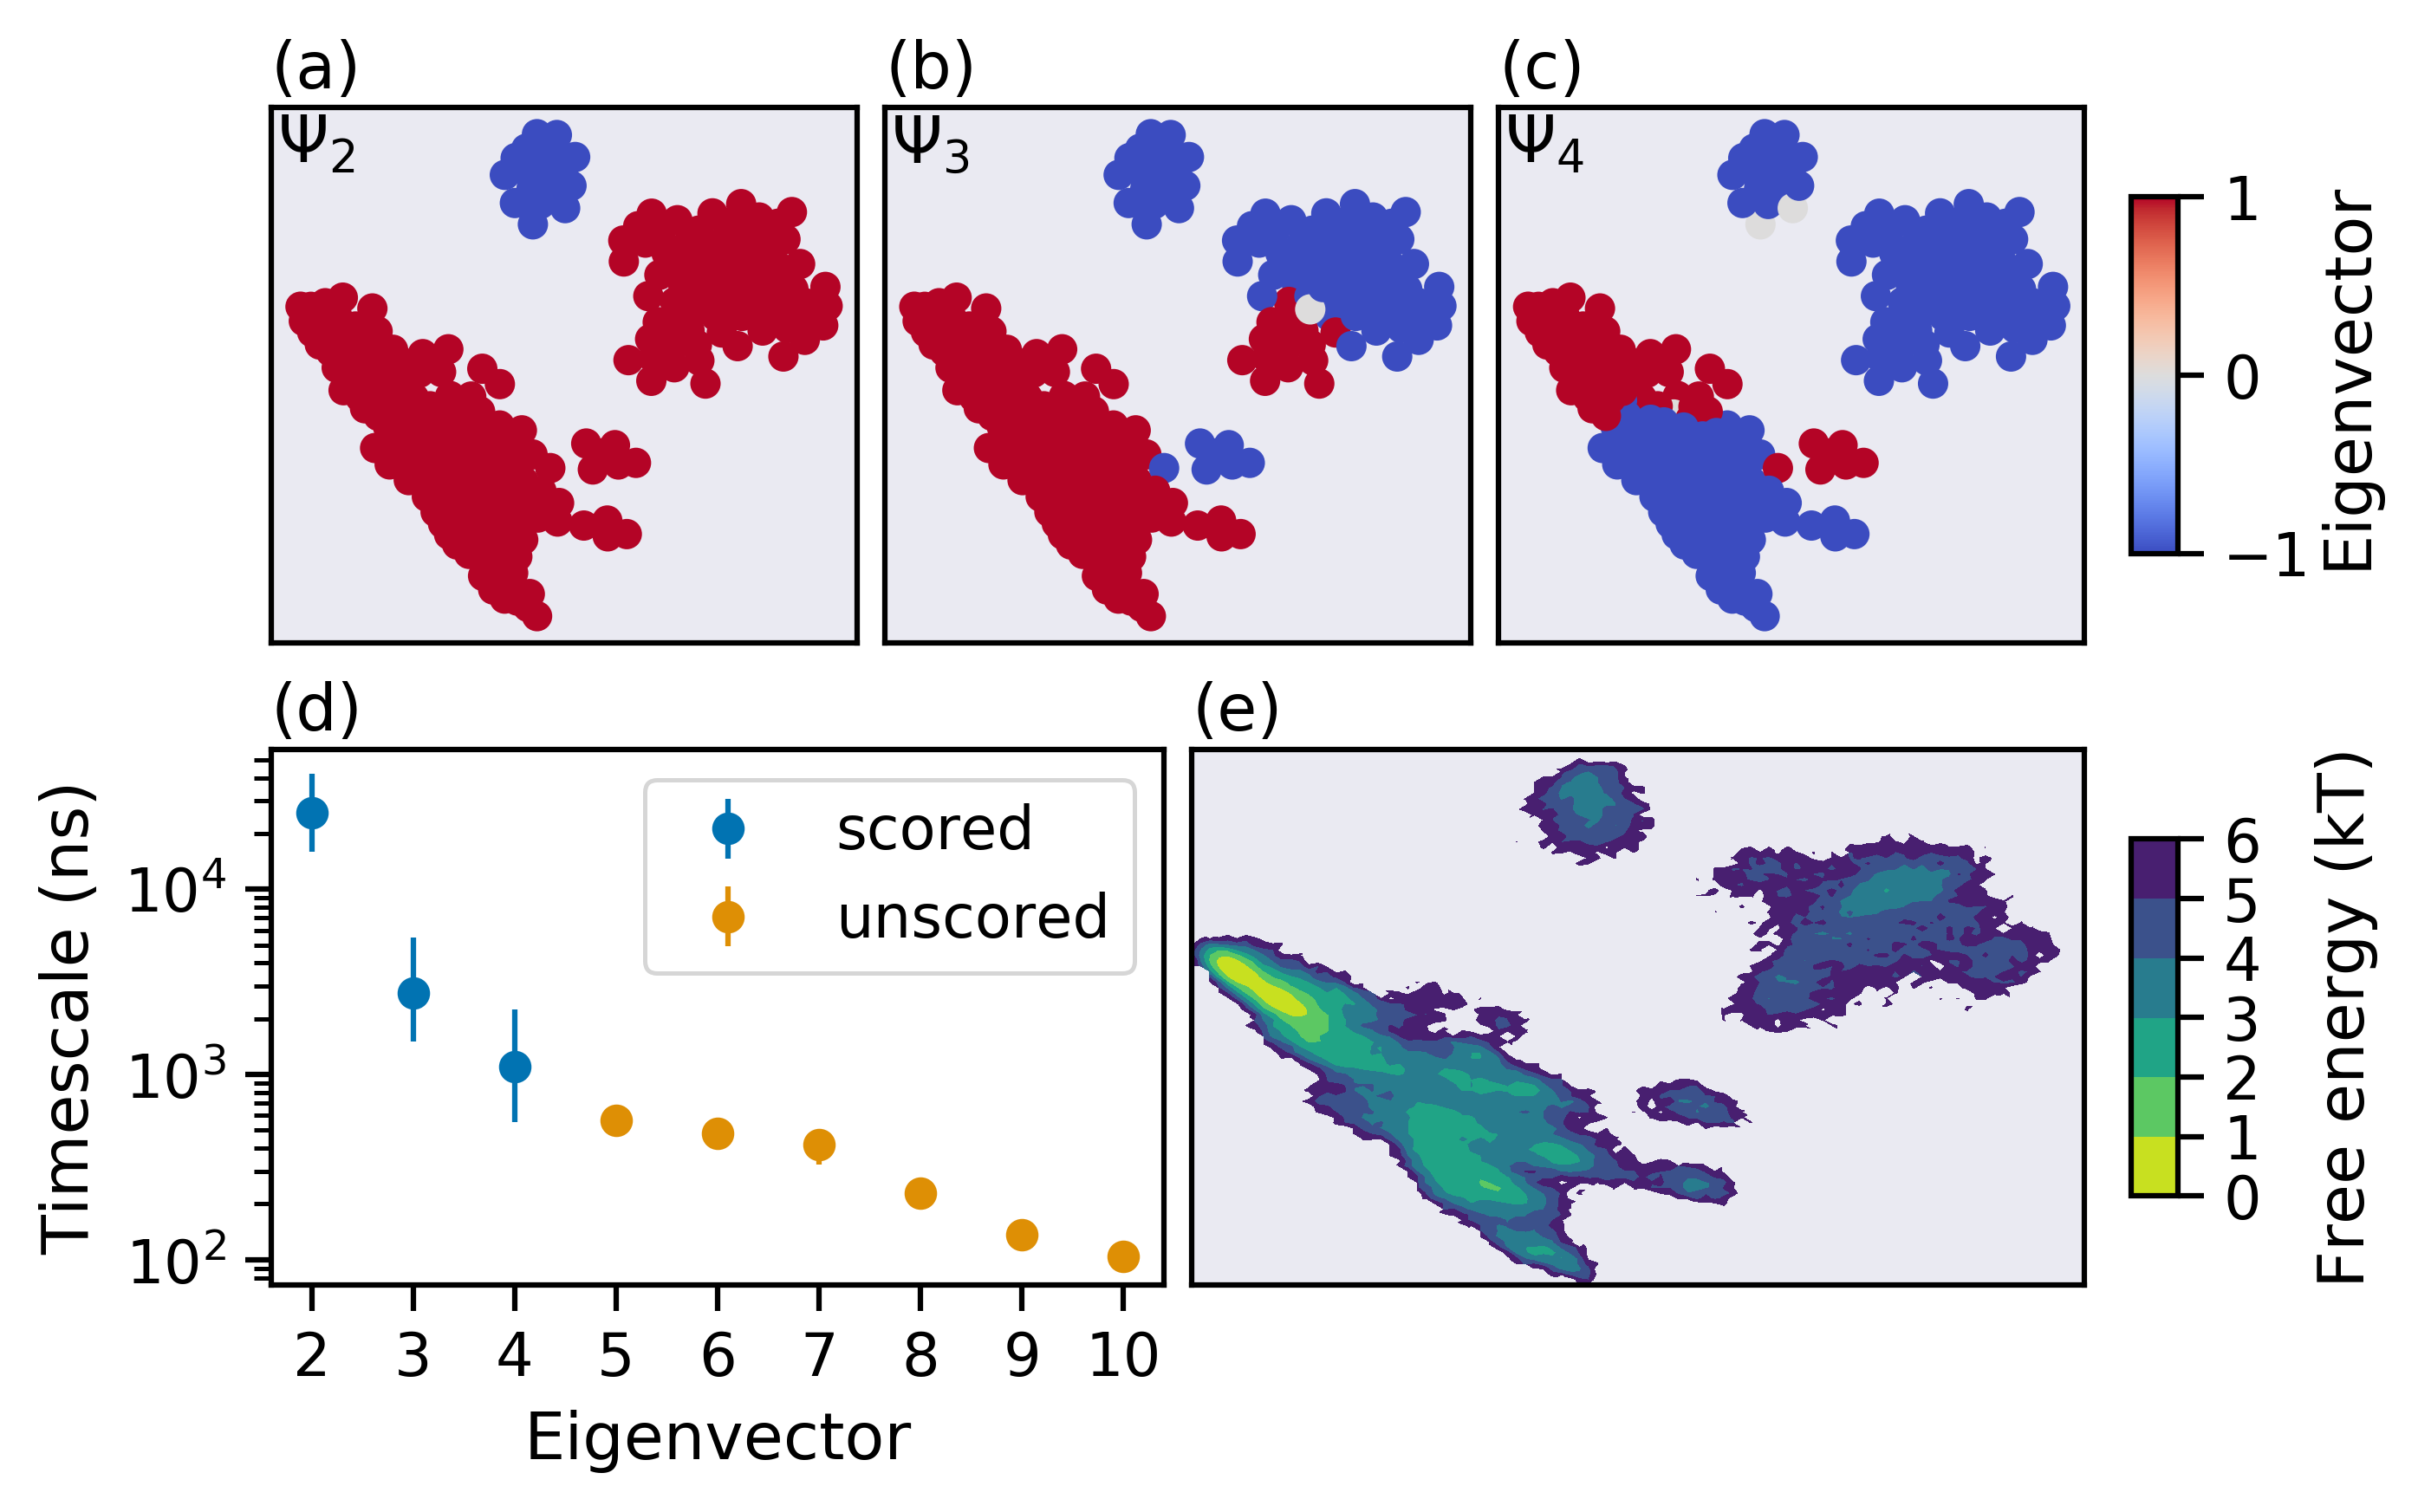
\includegraphics[width=0.8\textwidth]{chapters/msm_optimization/figures/aadh_msm_sens_1.png}
    \label{fig:aadh_msm_sens_1}
\end{figure}

Figure \ref{fig:aadh_msm_best} will serve as a base case for a number of sensitivity analyses, informed by the optimised response surface (figure \ref{fig:aadh_rsm_opt}) and eigenvalue spectrum (figure \ref{fig:aadh_its}). A summary of the hyperparameters for the base case and sensitivity cases are shown at the end of this section in table \ref{tab:aadh_final_msm_specs}. 

Sensitivity 1 changed the MSM lag time from $\SI{2}{\nano\second}$ to $\SI{20}{\nano\second}$ and is shown in figure \ref{fig:aadh_msm_sens_1}. As expected the absolute values of the implied timescales have increased, as has the relative separation between $t_{2}$ and $t_{3}$. 
% The values of relaxation timescales are summarised in table \ref{tab:sens_ts}.
This sensitivity case is included as,  while the sign structure is the same for the first and third relaxation process, it has changed for the second relaxation process.  Therefore the first, definitely slow, relaxation process is robust with respect to its sign structure. The second relaxation process which may or may not be dominant, changes its character as a function of the MSM lag time and will need to be further investigated. 

\begin{figure}
    \centering
    \caption[Sensitivity 2 MSM]{\textsc{Sensitivity 2 MSM}. This sensitivity used the best performing hyperparameters with a different value of $\chi$ to the base case. The hyperparameters were chosen to be $\chi= |\mathbf{r}_{1} - \mathbf{r}_{2}|$, $\tau = \SI{1}{\nano\second}, m=2, n=110$) and $\tau(\mathrm{MSM}) \SI{2}{\nano\second}$. See caption of figure \ref{fig:aadh_msm_best} for details.}
    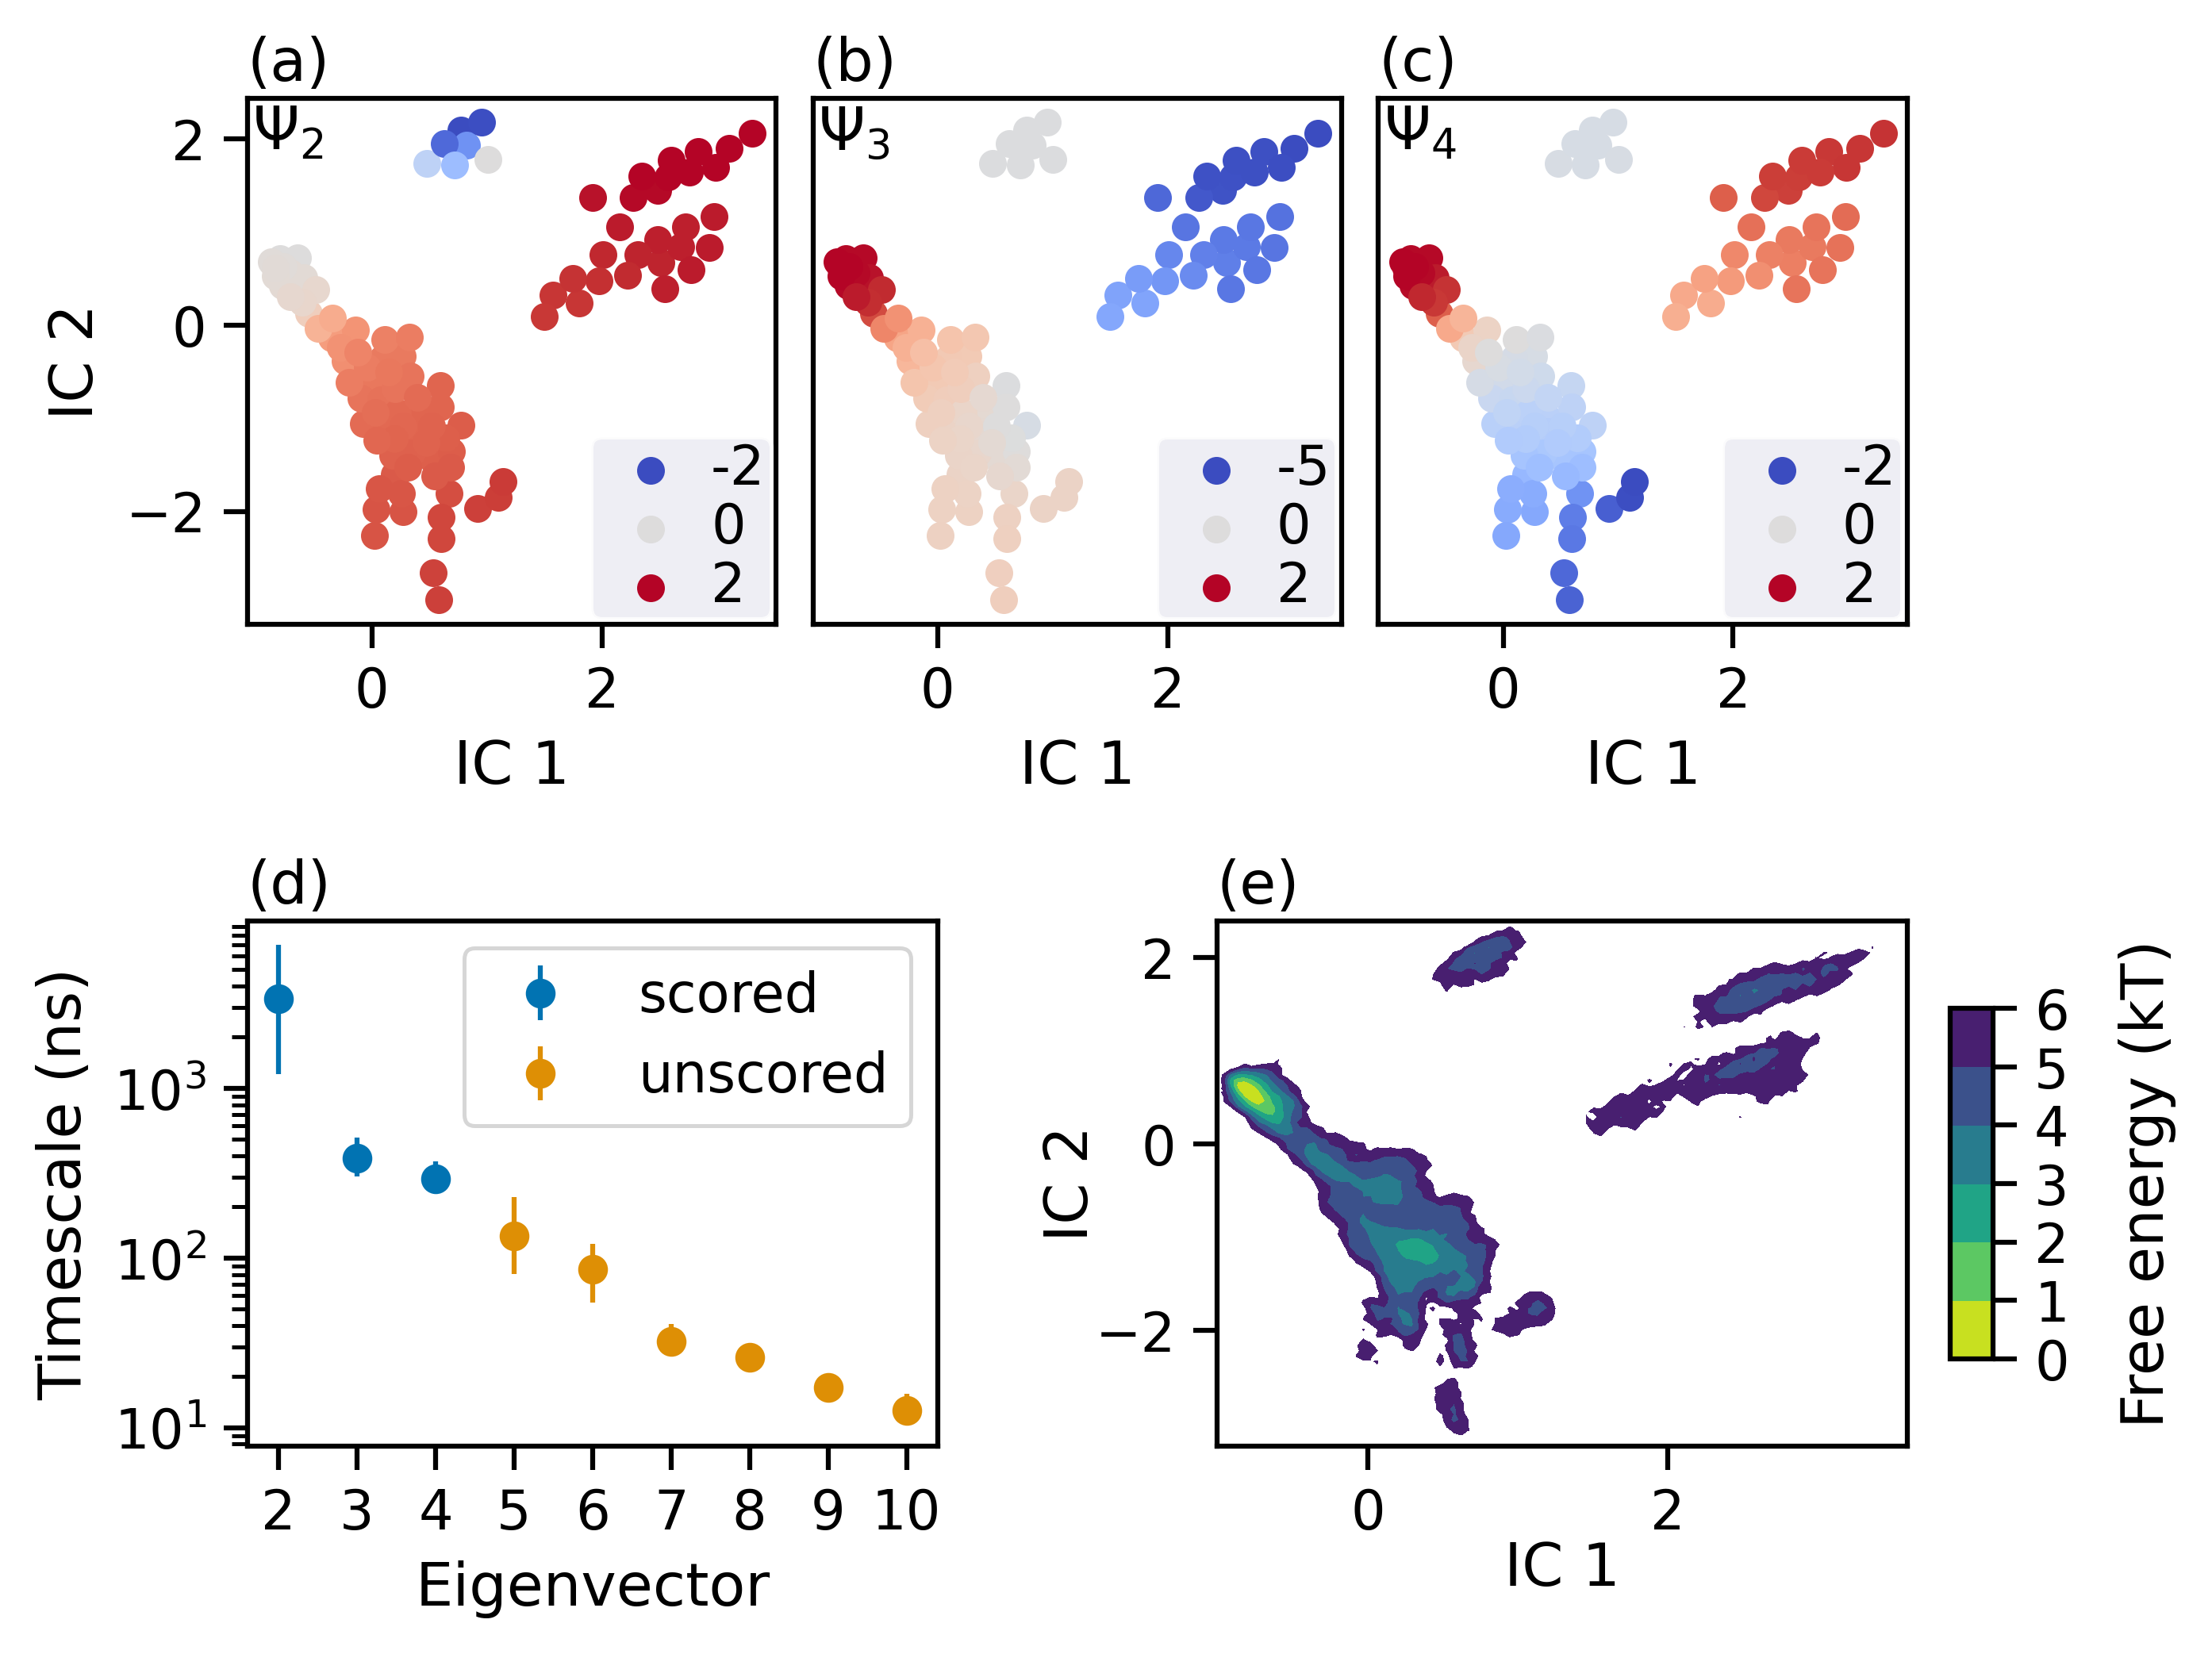
\includegraphics[width=0.8\textwidth]{chapters/msm_optimization/figures/aadh_msm_sens_2.png}
    \label{fig:aadh_msm_sens_2}
\end{figure}

Sensitivity 2 changed the hyperparameters to the best performing set with the interatomic distances feature ($\chi = |\mathbf{r}_{1} - \mathbf{r}_{2}|, \tau = \SI{1}{\nano\second}, m=2, n=110$) and is shown in figure \ref{fig:aadh_msm_sens_2}.  This was justified because of the similarity in the maximum response values (base case: $\mu=3.56 \pm 0.18$, sensitivity 2: $\mu=3.44 \pm 0.35$). There is a clear similarity between sensitivity 2 and the base case in both the free energy surface and the first relaxation processes' timescale ($t_{2} = \SI{2.7}{\micro\second}$ cf.$t_{2} = \SI{2.2}{\micro\second}$ in the base case) and sign structure of $\Psi_{2}$ and $\Psi_{3}$.  There is also a greater separation in timescales between $t_{2}$ and $t_{3}$ ($t_{2}/t_{3} \simeq 6$) than the base case ($t_{2}/t_{3} \simeq 2$). Taken together these two observations suggest that the interatomic distances potentially resolve the first relaxation processes similarly. 

\begin{figure}
    \centering
    \caption[Sensitivity 3 MSM]{\textsc{Sensitivity 3 MSM}. The hyperparameters were the same as the base case but with a  longer TICA lag time $\tau = \SI{85}{\nano\second}$.  See caption of figure \ref{fig:aadh_msm_best} for details.}
    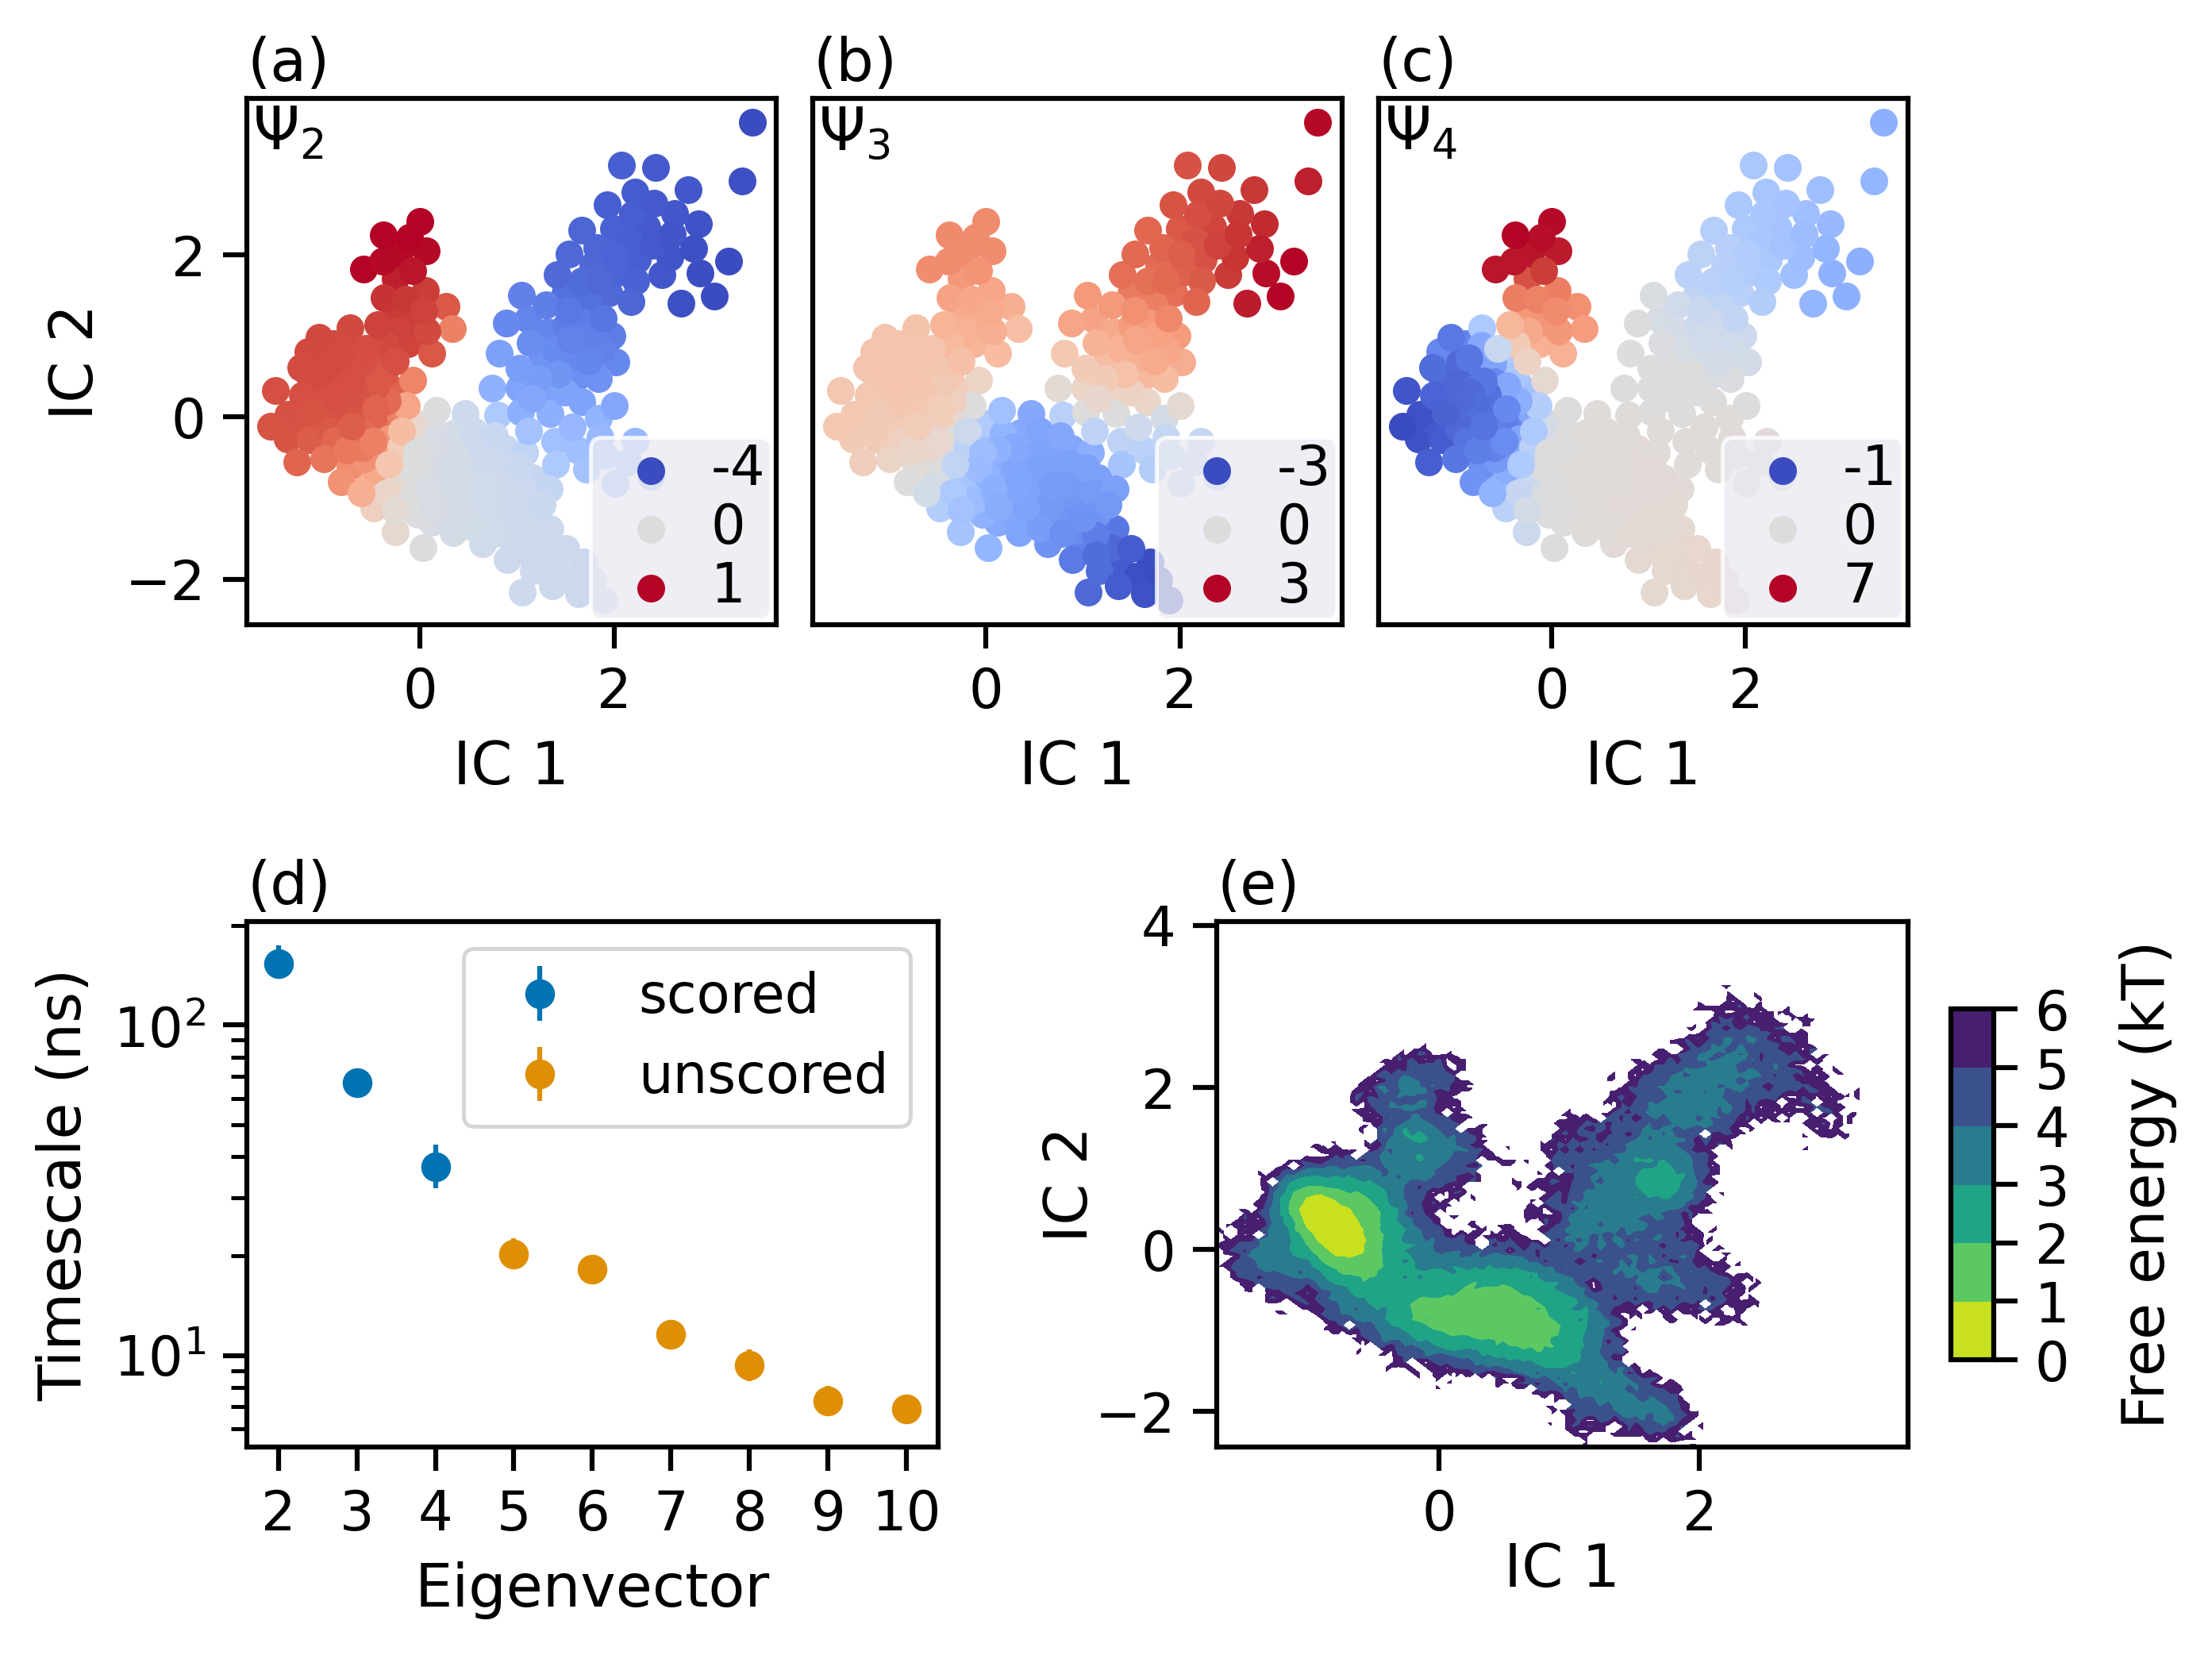
\includegraphics[width=0.8\textwidth]{chapters/msm_optimization/figures/aadh_msm_sens_3.png}
    \label{fig:aadh_msm_sens_3}
\end{figure}

\begin{figure}
    \centering
    \mycaption[Comparison of the base case and sensitivity 3 TICA eigenvectors]{\textsc{Comparison of the base case and sensitivity 3 TICA eigenvectors}. The TICA lag time for the base case was $\tau=\SI{10}{\nano\second}$ (blue) and for sensitivity 3 was $\tau=\SI{85}{\nano\second}$ (orange). The individual elements correspond to the weights associated with each of the $116$ dihedral angle features. Only the absolute values are shown. The elements were ordered according to the absolute value of the elements in the base case for each TICA component to highlight the differences. The normalized overlap between the base case ($\mathbf{v}_{1}$) and sensitivity three ($\mathbf{v}_{2}$) is calculated as $\mathbf{v}_{1}\cdot\mathbf{v}_{2}/|\mathbf{v}_{1}||\mathbf{v}_{2}|$.}
    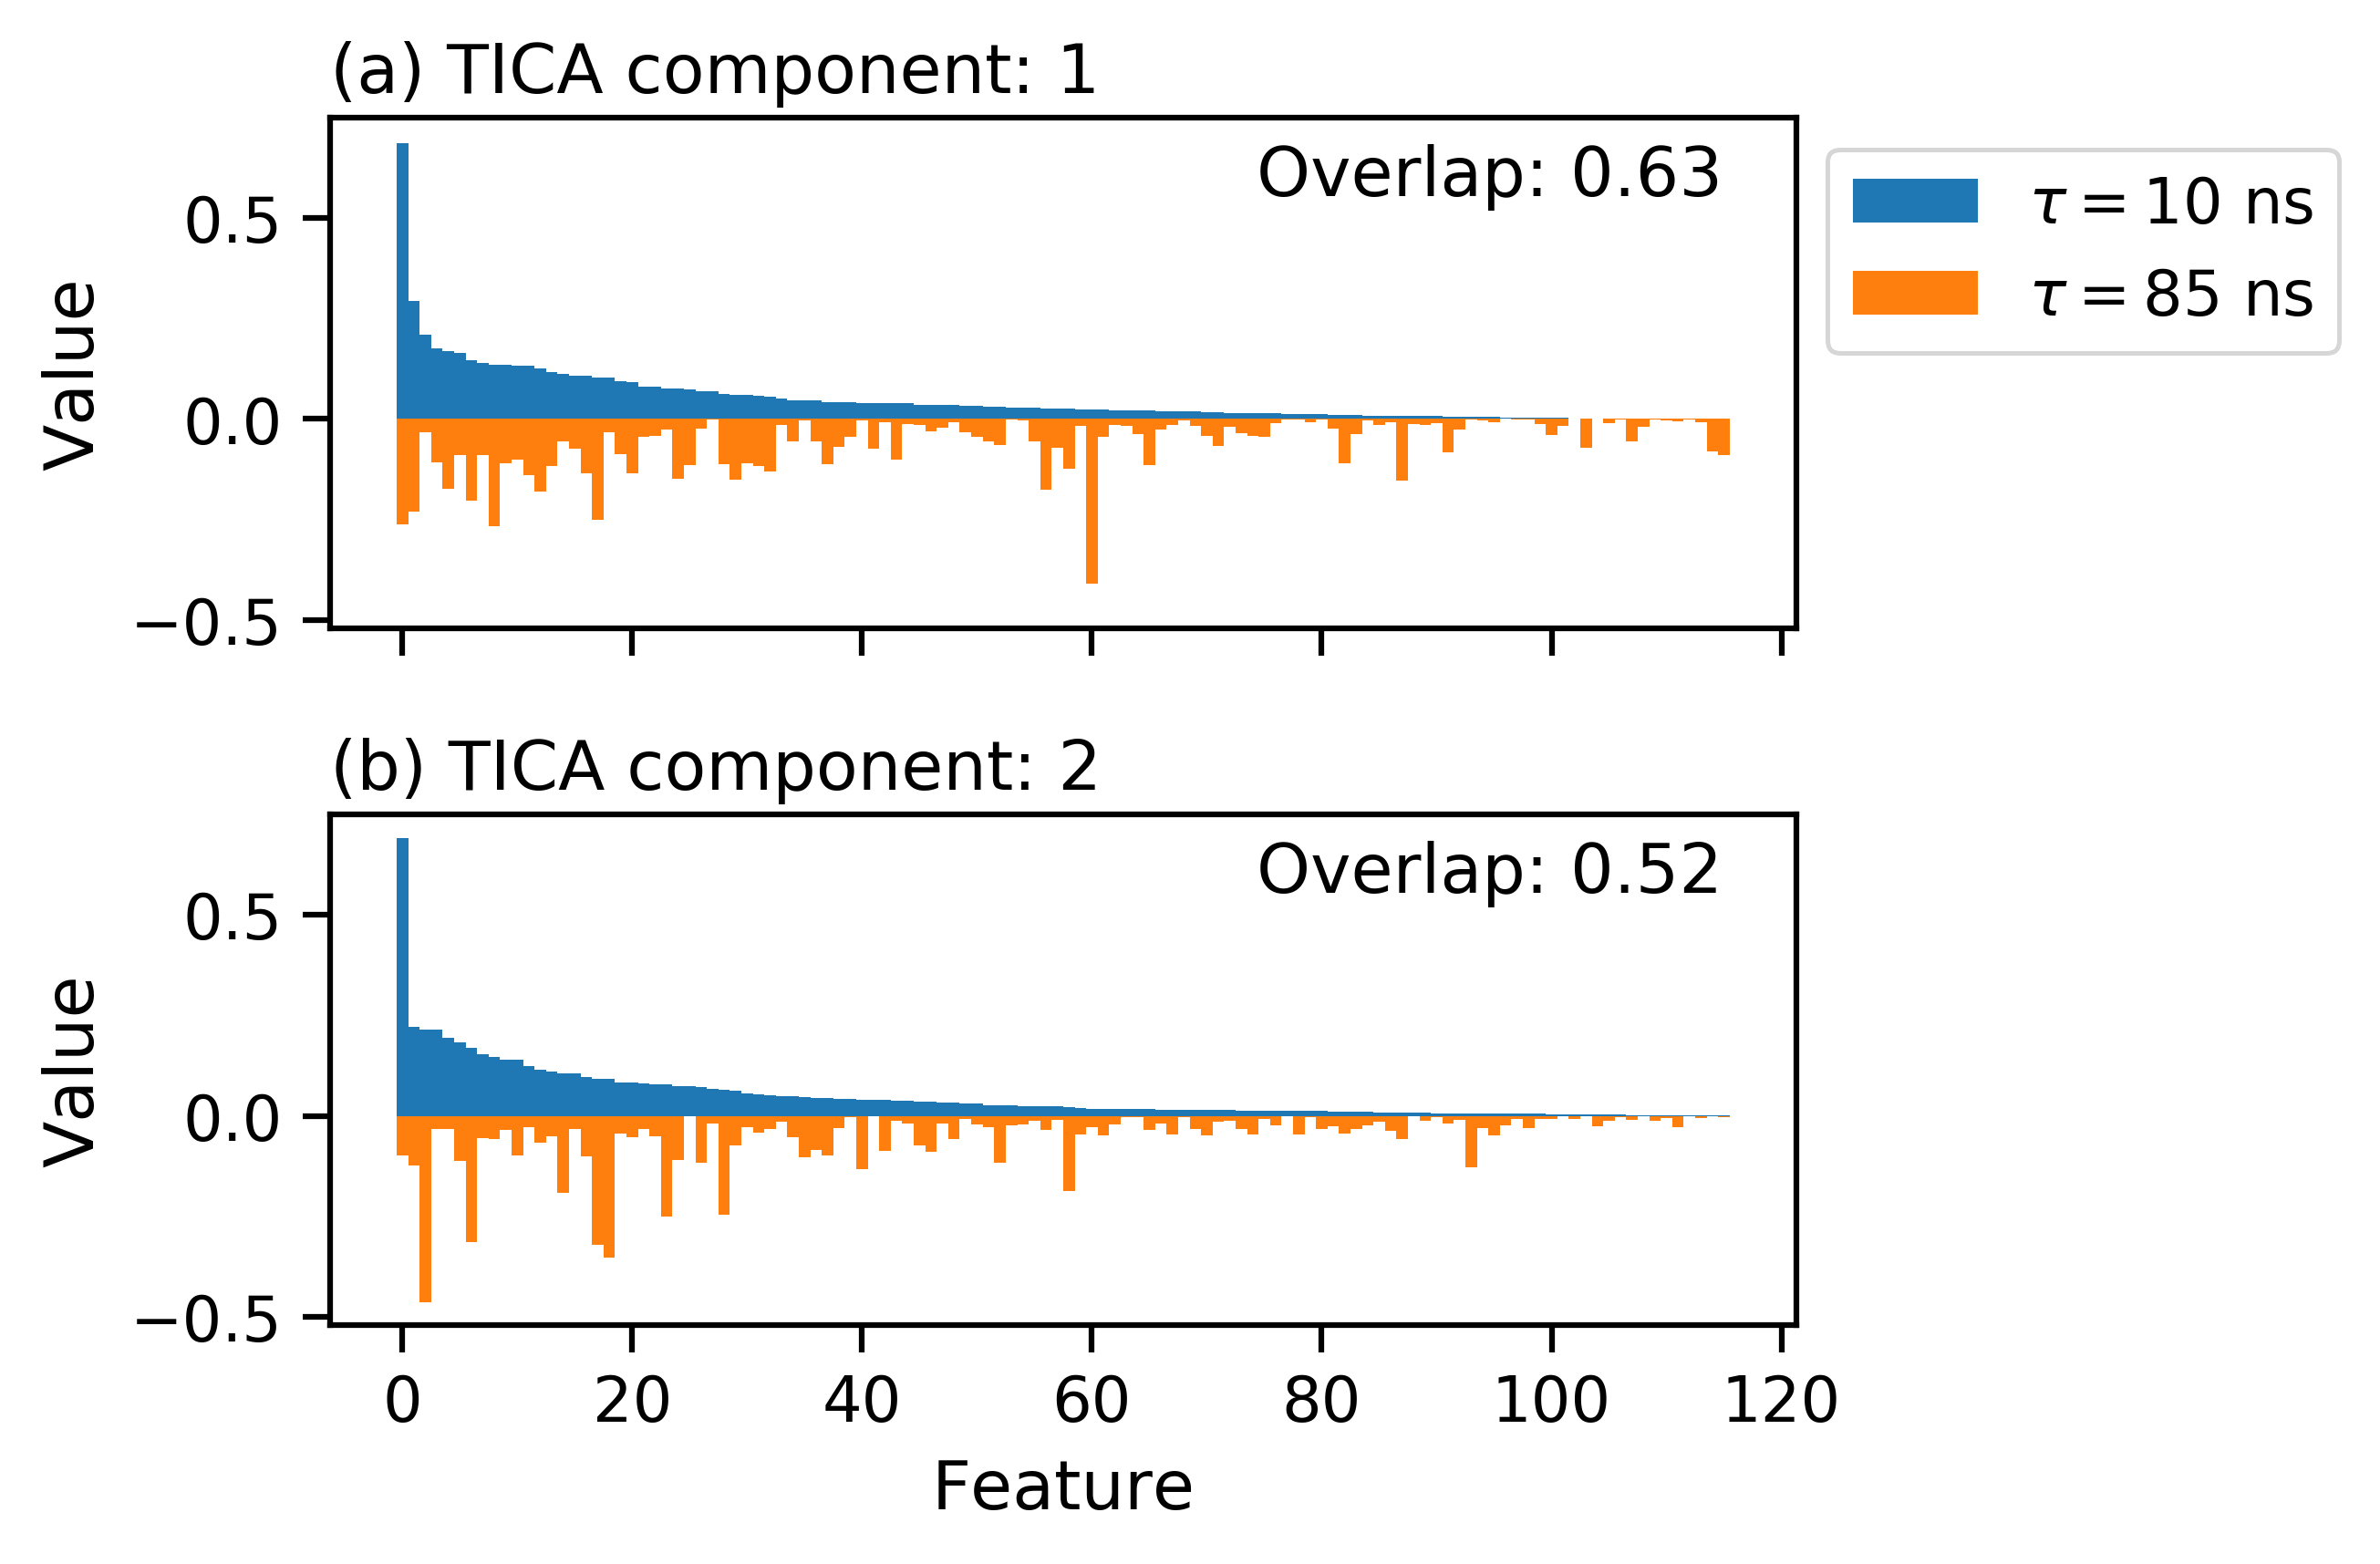
\includegraphics[width=0.8\textwidth]{chapters/msm_optimization/figures/aadh_msm_sens_3_tica.png}
    \label{fig:aadh_msm_sens_3_tica}
\end{figure}

Sensitivity 3, changed the value of $\tau$ to $\SI{85}{\nano\second}$ from to $tau = \SI{10}{\nano\second}$ in the base case and is shown in figure \ref{fig:aadh_msm_sens_3}.   This value of $\tau$ was chosen because the response at this point had the smallest  overlap with the incumbent (base case: $\mu=3.56 \pm 0.18$, sensitivity 3: $\mu=3.30 \pm 0.24$). It was the least similar of the values with overlapping distributions. Here there is a distinct difference in the absolute values of the timescales and the free energy surface compared to the base case. To further delineate the difference between the two TICA representations, figure \ref{fig:aadh_msm_sens_3_tica} shows the difference between the first two TICA components. The  TICA components of the base case are shown in blue with the magnitude of the individual elements (corresponding to the $116$ dihedral angle features) ordered in decreasing value. The corresponding elements for sensitivity 3 are shown in orange with the sign flipped. The normalized overlap between the two TICA components of the base case and sensitivity 3 are $0.63$ and $0.56$  for the first and second TICA components respectively. This is due to the different weights attached to each dihedral angle features. This suggest that the two TICA eigenvectors represent a qualitatively and quantitatively different model. Where this change comes in the response surface and and what the corresponding values of the response will determine whether this an example of the Roshomon effect. 


\begin{table}
    \centering
    \mycaption[Markov lag time and hyperparameters of selected models]{\textsc{Markov lag time and hyperparameters of selected models}. These models are the base case and sensitivity models to be coarse grained in section \ref{sec:aadh_hmm}. }
    \begin{tabular}{|l|l|l|l|l|}
        \hline
        Parameter & Base case & Sensitivity 1 & Sensitivity 2 & Sensitivity 3 \\
        \hline\hline
        Markov lag time, $\tau(\textrm{MSM})$ & \SI{2}{\nano\second} &  \SI{20}{\nano\second}& \SI{2}{\nano\second}& \SI{2}{\nano\second} \\
        Feature, $\chi$ & $(\phi, \psi, \chi)$ & $(\phi, \psi, \chi)$ & $|\mathbf{r}_{1}-\mathbf{r}_2|$ & $(\phi, \psi, \chi)$ \\
        TICA lag time, $\tau$ & \SI{10}{\nano\second} & \SI{10}{\nano\second}&\SI{1}{\nano\second} &\SI{85}{\nano\second} \\
        TICA components, $m$ & $2$ & $2$ & $2$ & $2$ \\
        Cluster centres, $n$ & $310$ & $310$ & $110$ & $310$ \\
        \hline
    \end{tabular}
    \label{tab:aadh_final_msm_specs}
\end{table}

\section{Coarse grained model}\label{sec:aadh_hmm}

\begin{figure}
    \centering
    \mycaption[Hidden state selection of AADH with the ICL]{\textsc{Hidden state selection of AADH with the ICL}. The base case is shown in panel (a), and the three sensitivity cases  in panels (b) - (c).  The coloured bars show the components of the ICL: the log-likelihood ($-2LL$) term is in blue, the BIC penalty term,  $d\cdot\log{N_{\mathrm{obs}}}$, is shown in green, and the classification entropy penalty term, $2\cdot EN$, is shown in red. The values are scaled so the minimum for each case is $1$, this value is denoted with an arrow and labelled  with number of hidden states. Models which failed to converge are missing.}
    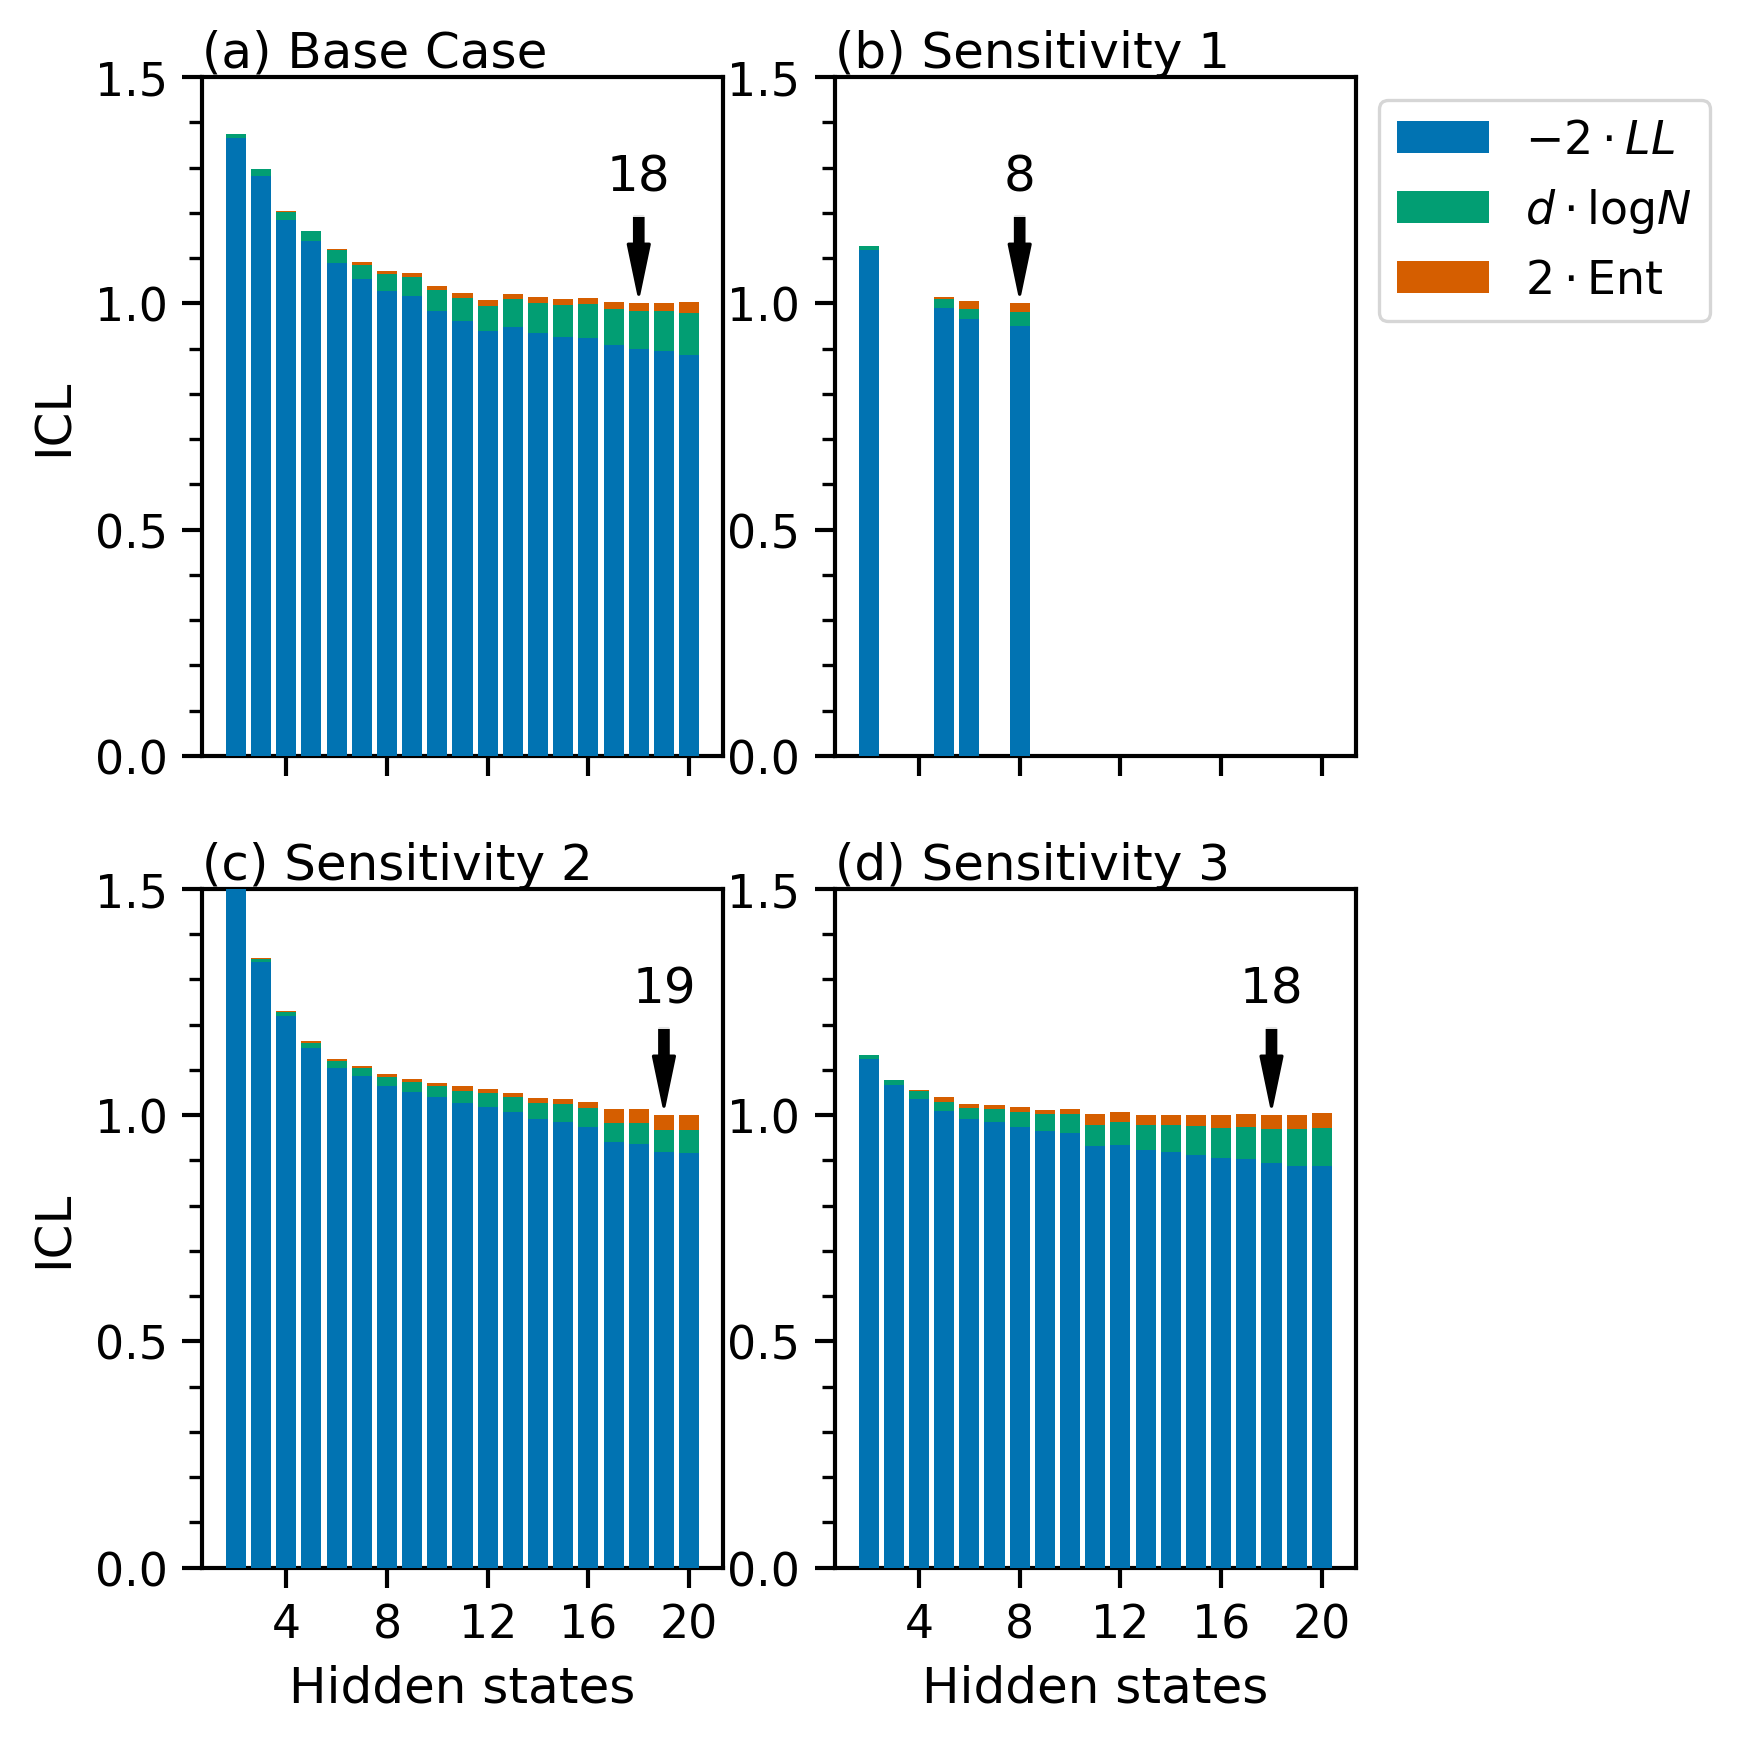
\includegraphics[width=0.8\textwidth]{chapters/aadh/figures/aadh_h_state_selection.png}
    \label{fig:aadh_h_selection_results}
\end{figure}

The aim of this section is to produce a coarse-grained picture of the conformational dynamics using a hidden Markov model. For each of the Markov state models defined in table \ref{tab:aadh_final_msm_specs}, maximum likelihood HMMs with between $2 - 20$ hidden states were estimated and the ICL calculated for each one. No striding of the data was performed. The number of hidden states was determined by the smallest value of the ICL ($g^{\mathrm{ICL}}$). For the selected number of hidden states a Bayesian HMM was estimated with four independent chains each with \num{4000} posterior samples, collected after \num{1000} burn-in steps. The trajectories were strided according to equation \ref{eqn:hmm_striding} to avoid optimistic bias in the error estimates\cite{trendelkamp-schroerEstimationUncertaintyReversible2015b}. Convergence of the samples was checked using the rank-normalized $\hat{R}$ statistic\cite{vehtariRanknormalizationFoldingLocalization2020} of the non-zero hidden transition matrix elements. If a converged Bayesian HMM could be estimated then a CK test was performed. 

Values of the ICL for each case is shown in figure \ref{fig:aadh_h_selection_results} which have been scaled for clarity. For reference the unscaled ICL values and the contribution due to the classification entropy are tabulated in table \ref{tab:aadh_h_state_selection}. The ICL behaves differently for AADH compared to the Prinz potential and selects large numbers of hidden states. As expected the log-likelihood increases with $g$ for each case, as does the BIC penalty term ($d\cdot\log{\left(N_{\mathrm{obs}}\right)}$, however unlike the results for the Prinz potential (figure \ref{fig:prinz_criteria_results}) the entropy term increases only negligibly. The number of selected states for each case is large (18, 8, 19, 18 for the base case and sensitivities 1 - 3 respectively) and in each case the number of strongly connected hidden states, $g^{\mathrm{s}}$, was less than the stipulated number of hidden states, $g$ (table \ref{tab:aadh_h_state_selection} also shows $g$ and $g^{\mathrm{s}}$ for all models). For example, the ICL selected $g^{\mathrm{ICL}}=18$ hidden states for the base case, figure \ref{fig:aadh_h_selection_results} panel (a). However, after re-estimating as a Bayesian HMM the largest strongly connected set within this model had  $g^{\mathrm{s}}=15$ hidden states. This was because, as described section \ref{sec:theory_hmm}, the trajectories were first strided so that the observations were approximately independent. This ensures that there are no optimistic biases in the resulting credible intervals. The striding interval was estimated from the data using  equation \ref{eqn:hmm_striding} which for the base case was $\Delta t = \SI{2}{\nano\second}$.  The effect of striding on connectivity was discussed in the context of the MSM count matrix in section \ref{sec:theory_count_mat} although the same principle applies here. Increasing the value of $\tau(\mathrm{MSM})$ will also decrease the connectivity of the count matrix if the hidden states are separated by timescales comparable to the new larger $\tau(\mathrm{MSM})$. This explains the failure to converge models 15 of the models at the longer lag time of sensitivity 1, figure \ref{fig:aadh_h_selection_results} panel (b).   


\begin{figure}
    \centering
    \mycaption[Base case HMM]{\textsc{Base case HMM}. Panel (a) shows the observed states (colour circles) in the space of the first two TICA components, IC 1 and IC 2. Each observed state, $j$ is assigned to the hidden state with the maximum a posteriori probability, i.e.  $\arg \max_{i} \mathrm{P}(h=i|s=j)$. Each colour corresponds to a hidden state, labelled $\numrange{1}{15}$. Panel (b) shows the median lifetimes of each state with \SI{95}{\percent} credible intervals. The horizontal width of the error bars and sizes of the markers are proportional to the stationary distribution of each hidden state. The Markov lag time is shown as a black horizontal line for comparison. Panel (c) shows the dominant hidden state relaxation process, $\Psi_{2}(h)$. Each observed state assigned to a hidden state $i$ is coloured according to the value of $\Psi_{2}(i)$ . Panel (d) shows the median implied timescales of the hidden state relaxation processes with \SI{95}{\percent} credible intervals. The Markov lag time is shown as a black horizontal line for comparison.}
    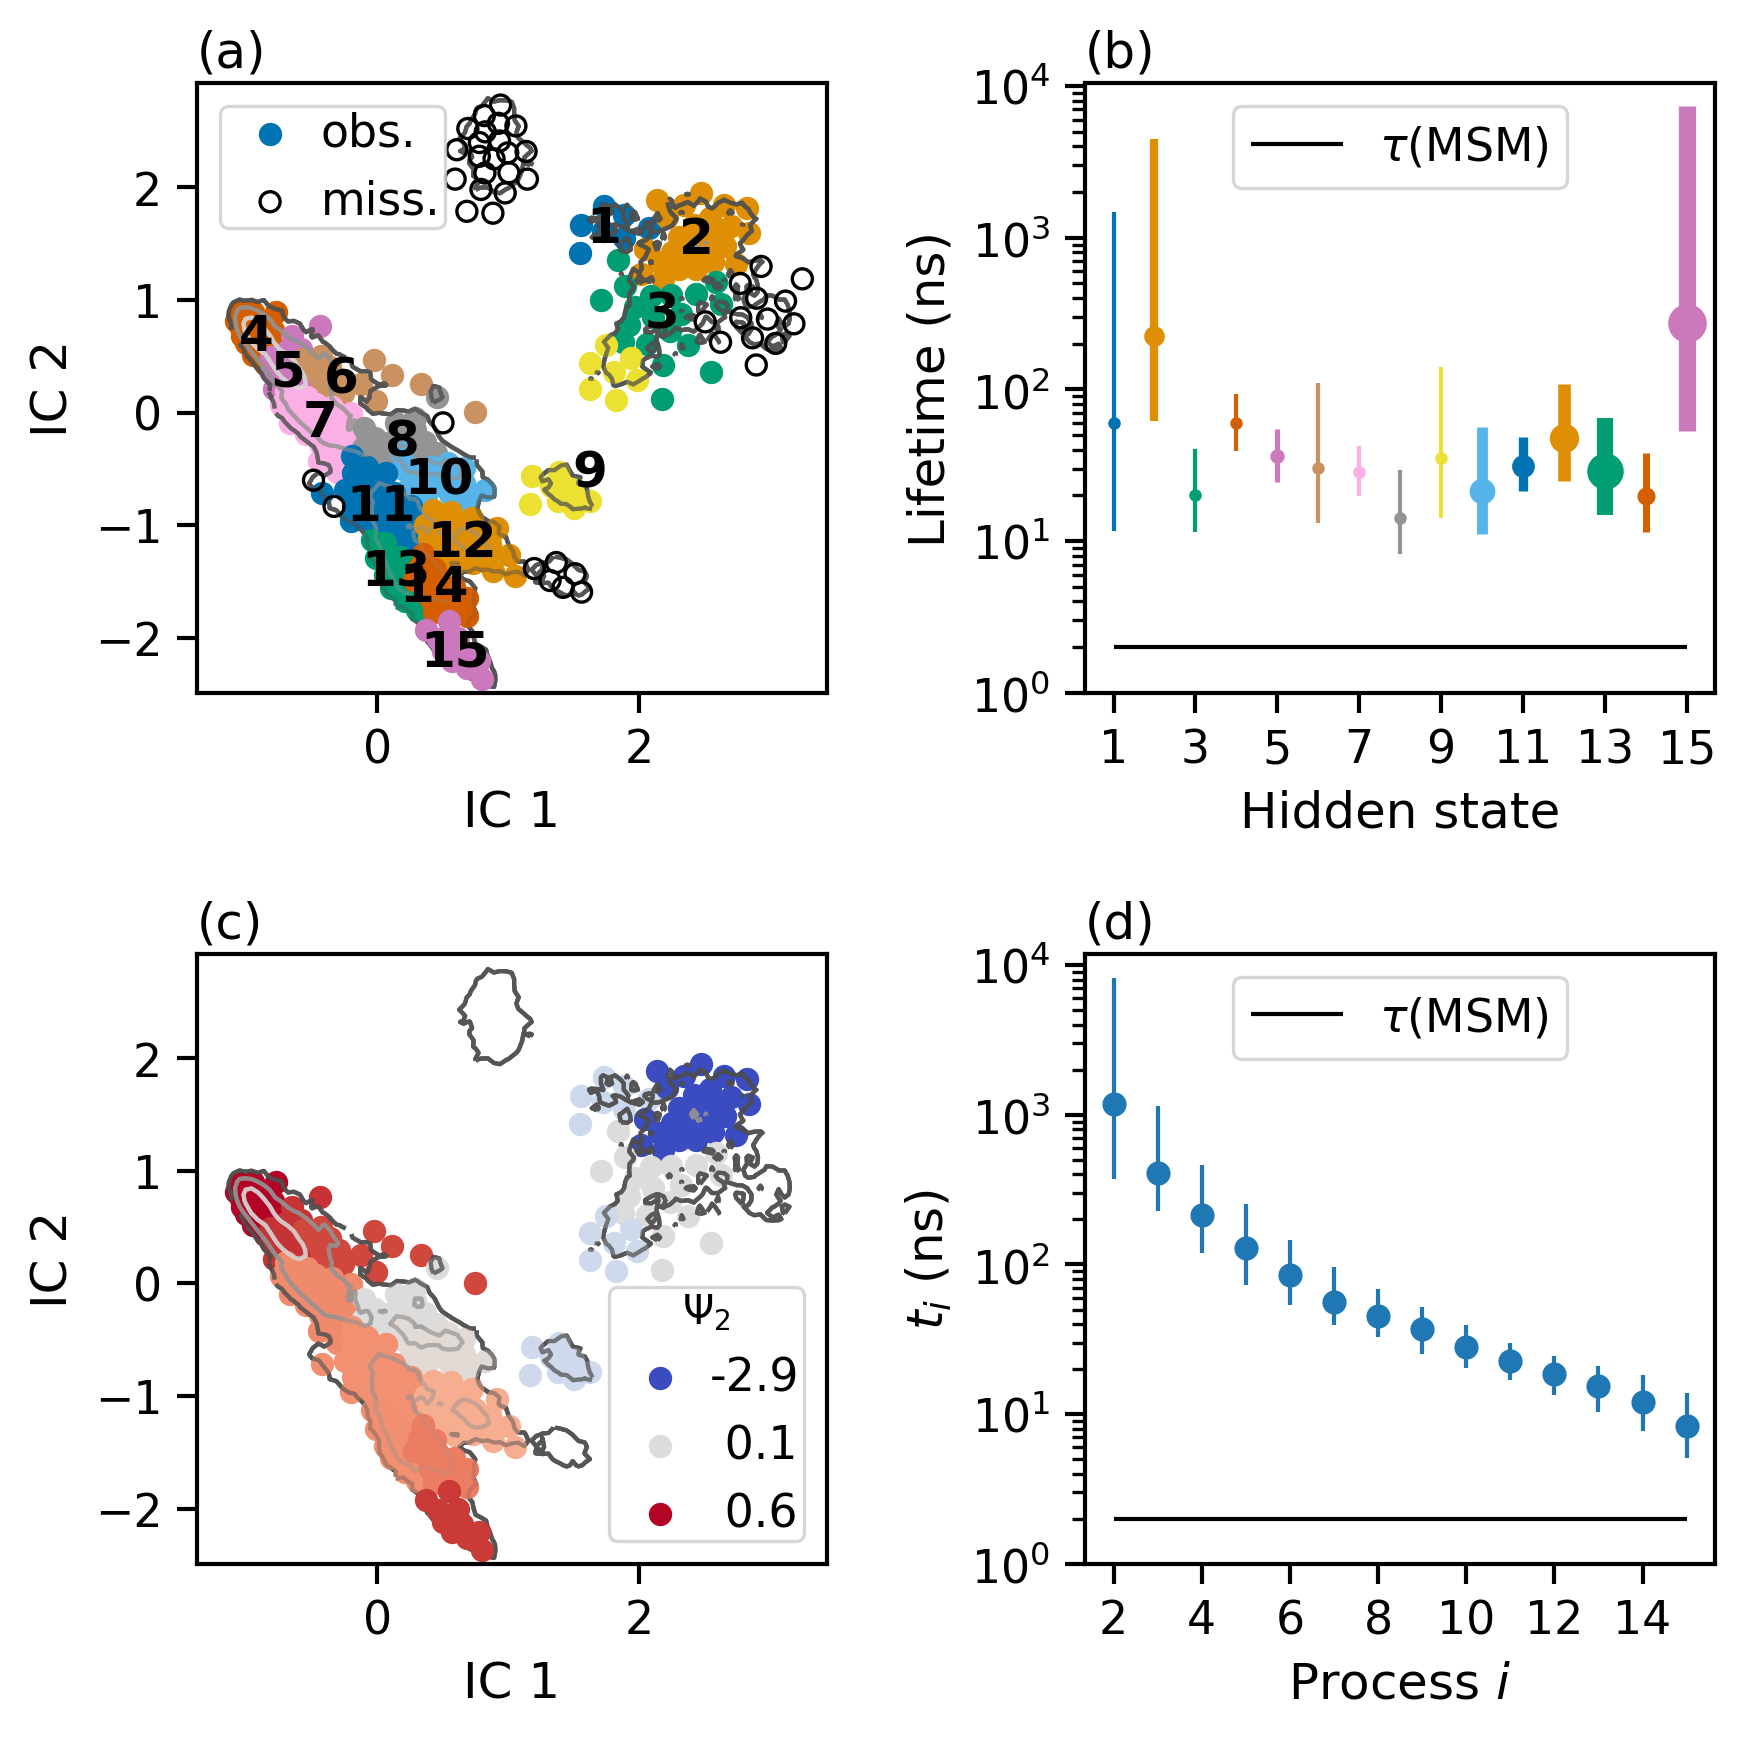
\includegraphics{chapters/aadh/figures/base_case_hmm.png}
    \label{fig:base_case_hmm}
\end{figure}

The base case with $g=18$ hidden states was re-estimated using Bayesian estimation so that the errors could be determined.  There was moderate convergence of the posterior chains with \SI{63}{\percent} of the transition matrix elements under the recommended threshold of $\hat{R}<1.01$ while the remaining elements had $\hat{R}<1.1$ (the full $\hat{R}$ statistics  are tabulated in table \ref{tab:aadh_base_case_rhat}). The final model is shown in figure \ref{fig:base_case_hmm}. Panel (a) shows the observed states assigned to the $15$ strongly connected hidden states in the space of the two TICA components (IC 1 and IC 2). There are $267$ out of $310$ observed states used in the model which constitute just under \SI{95}{\percent} of the observed states, the missing states are shown as unfilled black circles. However, the striding of the trajectories meant that only \SI{5}{\percent} of the total observations were used. All metastable state have short lifetimes in the range \SIrange{20}{60}{\nano\second} with two exceptions: state $h_2$ (\SI{223}{\nano\second} [\SIrange[range-phrase=-]{61.7}{4430}{\nano\second}]) and state $h_{15}$: (\SI{275}{\nano\second} [\SIrange[range-phrase=-]{53.4}{7400}{\nano\second}]). These two states are the two predominantly involved in the dominant relaxation process shown in panel (c) with a timescale of \SI{1180}{\nano\second} [\SIrange[range-phrase=-]{373}{8180}{\nano\second}]. This and the remaining timescales,  for comparison,  are shown in panel (d). 
There are two limitations to the base case hidden Markov model. First, the HMM could not be validated using the Chapman-Kolmogorov test because models with longer lag times resulted in further disconnections in the hidden state count matrix i.e., at lags of $\tau(\mathrm{MSM})> \SI{2}{\nano\second}$ the number of strongly connected hidden states was smaller than $15$. Second, missing observed states around $(\mathrm{IC 1}=0.9, \mathrm{IC 2}=2.3)$ (which collectively will be called $h_{-1}$) in figure \ref{fig:base_case_hmm} panel (a) are involved in the the dominant relaxation process in the  base case MSM, shown in figure \ref{fig:aadh_msm_best} panel (a). This process, with an implied timescale of \SI{2.21}{\micro\second} [\SIrange[range-phrase=-]{1.03}{5.21}{\micro\second}] is therefore not captured in the HMM.

No Bayesian HMM with ICL selected number of hidden states could be estimated for either sensitivity 1 (the base case with $\tau(\mathrm{MSM})=\SI{20}{\nano\second}$) or for sensitivity 3 (the  base case with $\tau = \SI{85}{\nano\second}$) because the trajectory striding required for accurate error estimation resulted in disconnected count matrix.  

\begin{figure}
    \centering
    \mycaption[Sensitivity 2 HMM]{\textsc{Sensitivity 2 HMM}.  Panel (a) shows the observed states (colour circles) in the space of the first two TICA components, IC 1 and IC 2. Each observed state, $j$ is assigned to the hidden state with the maximum a posteriori probability, i.e.  $\arg \max_{i} \mathrm{P}(h=i|s=j)$. Each colour corresponds to a hidden state, labelled \numrange{1}{13}. Panel (b) shows the median lifetimes of each state with \SI{95}{\percent} credible intervals. The horizontal width of the error bars and sizes of the markers are proportional to the stationary distribution of each hidden state. The Markov lag time is shown as a black horizontal line for comparison. Panel (c) shows the dominant hidden state relaxation process, $\Psi_{2}(i)$. Each observed state assigned to a hidden state $i$ is coloured according to the value of $\Psi_{2}(i)$ . Panel (d) shows the median implied timescales of the hidden state relaxation processes with \SI{95}{\percent} credible intervals. The Markov lag time is shown as a black horizontal line for comparison. }
    \label{fig:sensitivity_2_bhmm}
    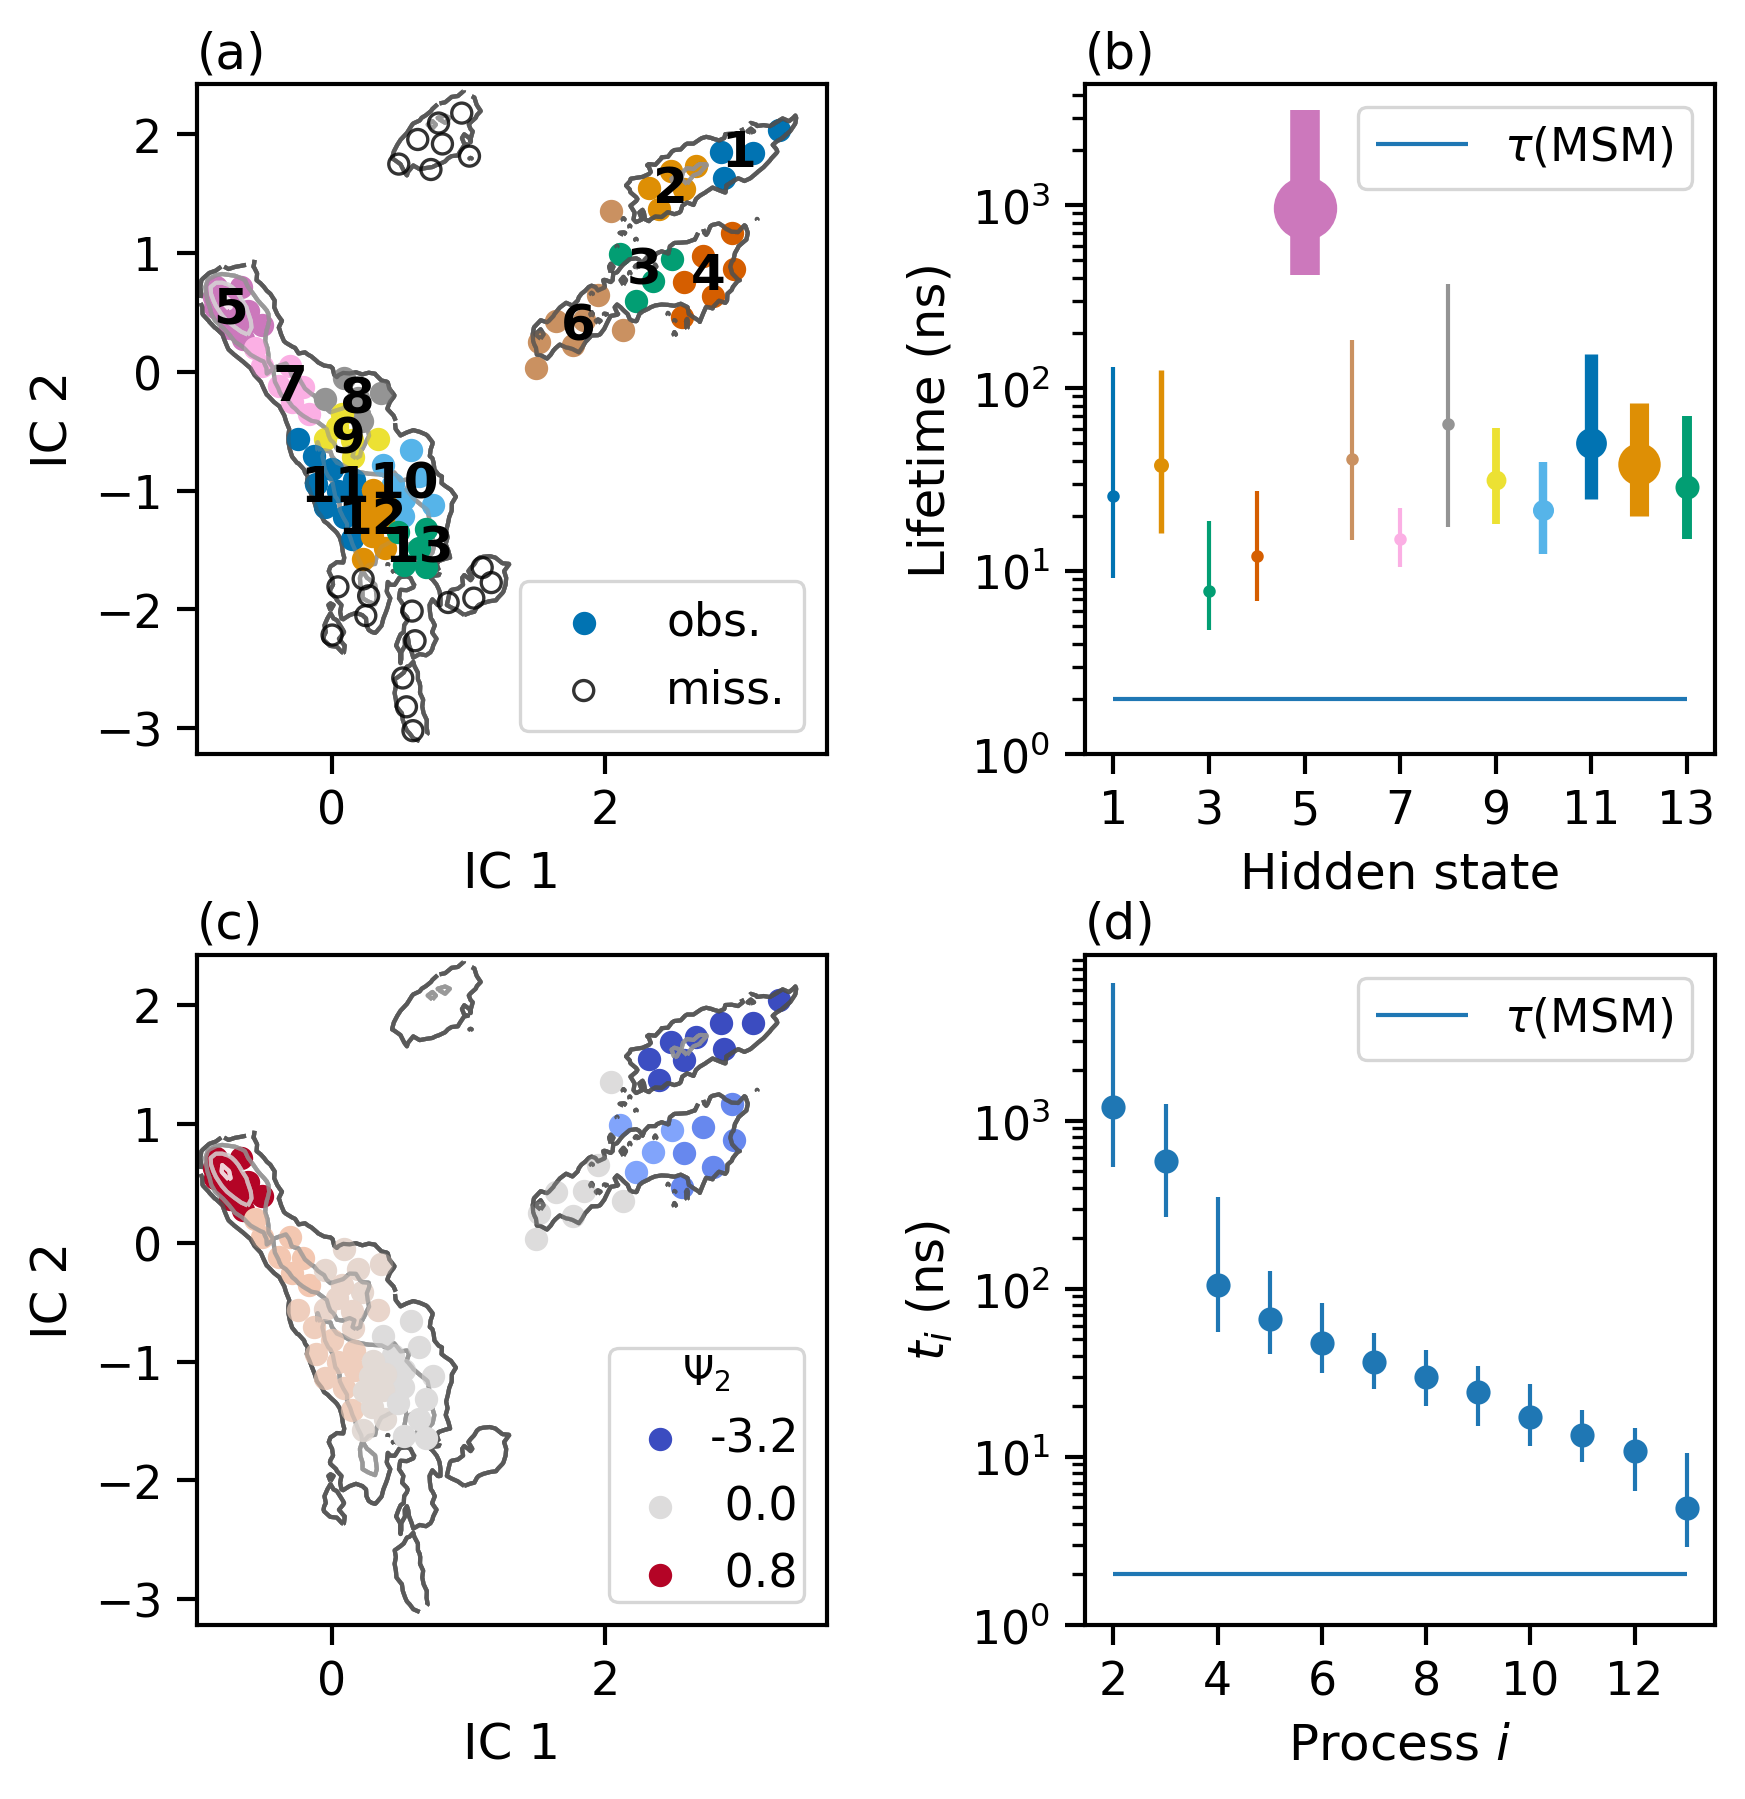
\includegraphics[width=0.8\textwidth]{chapters/aadh/figures/sensitivity_2_hmm.png}
\end{figure}

equation \ref{eqn:hmm_striding} which for the base case was $\Delta t = \SI{2}{\nano\second}$

A Bayesian HMM was estimated for sensitivity 2 which, after striding by  $\SI{2}{\nano\second}$ according to equation \ref{eqn:hmm_striding}, resulted in only $13$ hidden states forming a strongly connected set. Convergence of the model was mixed, \SI{60}{\percent} of the transition matrix elements were under the recommended threshold of $\hat{R}<1.01$,  however the remaining elements were unconverged with values up to $1.3$. The full list of $\hat{R}$ statistics can be found in table \ref{tab:sens_2_gelman_rubin}. The final model is shown in figure \ref{fig:sensitivity_2_bhmm}. Panel (a) shows the assignment of the observed states to the $13$ hidden states. Only $89$ of the $110$ observed states were used in the model (the missing states are shown as unfilled circles) constituting over \SI{92}{\percent} of the observed states. However, due to the striding only \SI{4}{\percent} of the observations were used. The hidden state lifetimes are shown in panel (b). All hidden states were short-lived with median lifetimes between \SIrange{8}{64}{\nano\second} except for state $h_5$, the most populous state, which has a lifetime of \SI{961}{\nano\second} [\SIrange[range-phrase=-]{416}{3310}{\nano\second}]. The dominant relaxation process, panel (c), involves population transfer between state $h_{5}$ and the four short-lived states $h_{1} - h_{4}$ with an implied timescale of \SI{1210}{\nano\second} [\SIrange[range-phrase=-]{533}{6590}{\nano\second}]. This and the remaining implied timescales are shown in panel (d). 

The sensitivity 2 HMM suffers from the same drawbacks as the the base case model and for the same reasons: the model could not be validated by the CK test and it is missing observed states important in the dominant relaxation process identified in the corresponding MSM, shown in figure \ref{fig:aadh_msm_sens_2}. The collection of observed states in the region $(\mathrm{IC 1}=0.8, \mathrm{IC 2}=1.9)$ (which collectively will be called $h_{-1}$) in figure \ref{fig:sensitivity_2_bhmm} panel (a) are involved in the the dominant process in the  base case MSM, shown in figure \ref{fig:aadh_msm_sens_2} panel (a). This process, with an implied timescale of \SI{2.69}{\micro\second} [\SIrange[range-phrase=-]{1.35}{4.61}{\micro\second} is therefore not captured in the HMM.

\section{Conformational landscape of AADH}\label{sec:aadh_landscape}

\begin{figure}
    \centering
    \mycaption[Donor-acceptor distances of the hidden states]{\textsc{Donor-acceptor distances of the hidden states}. The mean and \SI{95}{\percent} quantiles of the distribution for the OD1---C1 and OD2---C1  for each hidden state in the base case (panels (a) and (c) respectively) and sensitivity 2 (panels (b) and (d) respectively) HMMs. The colour scheme matches the colours in figures \ref{fig:base_case_hmm} and \ref{fig:sensitivity_2_bhmm}. In addition, the missing states $h_{-1}$ are shown in black. The horizontal blue line is distance estimated using QM/MM in reference \cite{ranaghanInitioQMMM2017}.}
    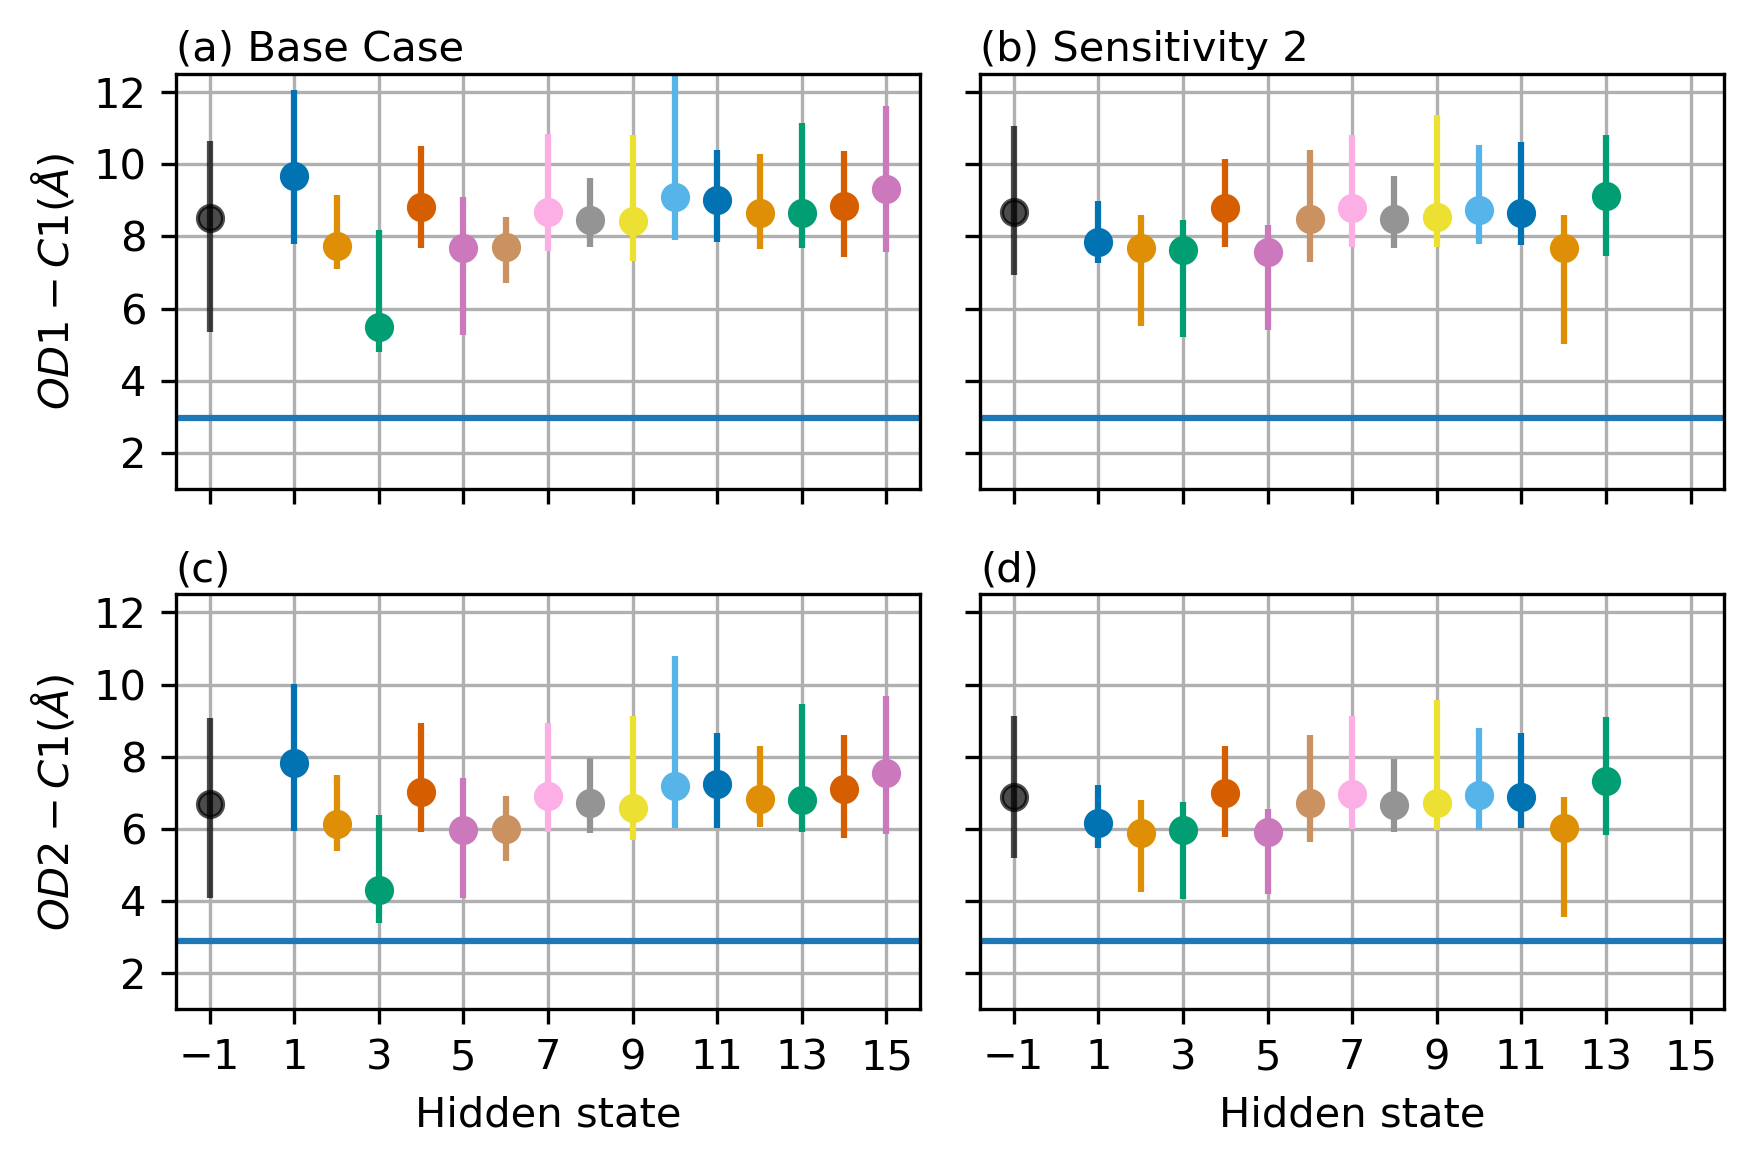
\includegraphics[width=0.8\textwidth]{chapters/aadh/figures/bond_dist_h_states.png}
    \label{fig:addh_bond_dist_h_state}
\end{figure}

Although the validity of the base case and sensitivity 2 models as a description of the dynamics has not been established, understanding their implications for the conformational dynamics will complete their description and help guide further work in this area. 

As already established in section \ref{sec:aadh_validation} the sampled conformations in the D active site do not correspond to reactive conformations established in QM/MM studies.  However, within the sampled conformations the base case HMM resolves hidden states with variable degrees of reactive character as determined  by their acceptor-donor bond lengths (TTW-C1---Asp128-OD1/OD2 bond length) as shown in figure \ref{fig:addh_bond_dist_h_state}. The base case $h_{3}$ has a smaller donor-acceptor bond length to both both acceptors (OD1 and OD2), \SI{5.5}{\angstrom} and \SI{4.3}{\angstrom} respectively. The other base case hidden states (including the `missing' state $h_{-1}$) have donor-acceptor lengths between \SIrange{7.7}{9.7}{\angstrom} to OD1 and \SIrange{6.0}{7.8}{\angstrom} to OD2. 

\begin{figure}[p]
    \centering
    \mycaption[Base case HMM as a network]{\textsc{Base case HMM as a network}. Each orange circle is a hidden state with area proportional to its stationary distribution. Arrows connect states $i$ and $i$ where the flux, $\tilde{\pi}_{i}\tilde{T}_{ij}$, is greater than $\SI{0.01}{\percent}$. The orientation of the states mirrors their position in the TICA plane. Representative structures are shown for $h_{-1}, h_{2}, h_{3}, h_{4}, h_{13}, h_{15}$. The most important TICA dihedrals are shown in blue. The yellow bonds are the C---OD1/OD2 on the Asp 128 residue (D128) and the CI---HI2/3 bonds on TTW 109 (X109). Rates of interconversion are shown for those states connected to $h_{3}$. }
    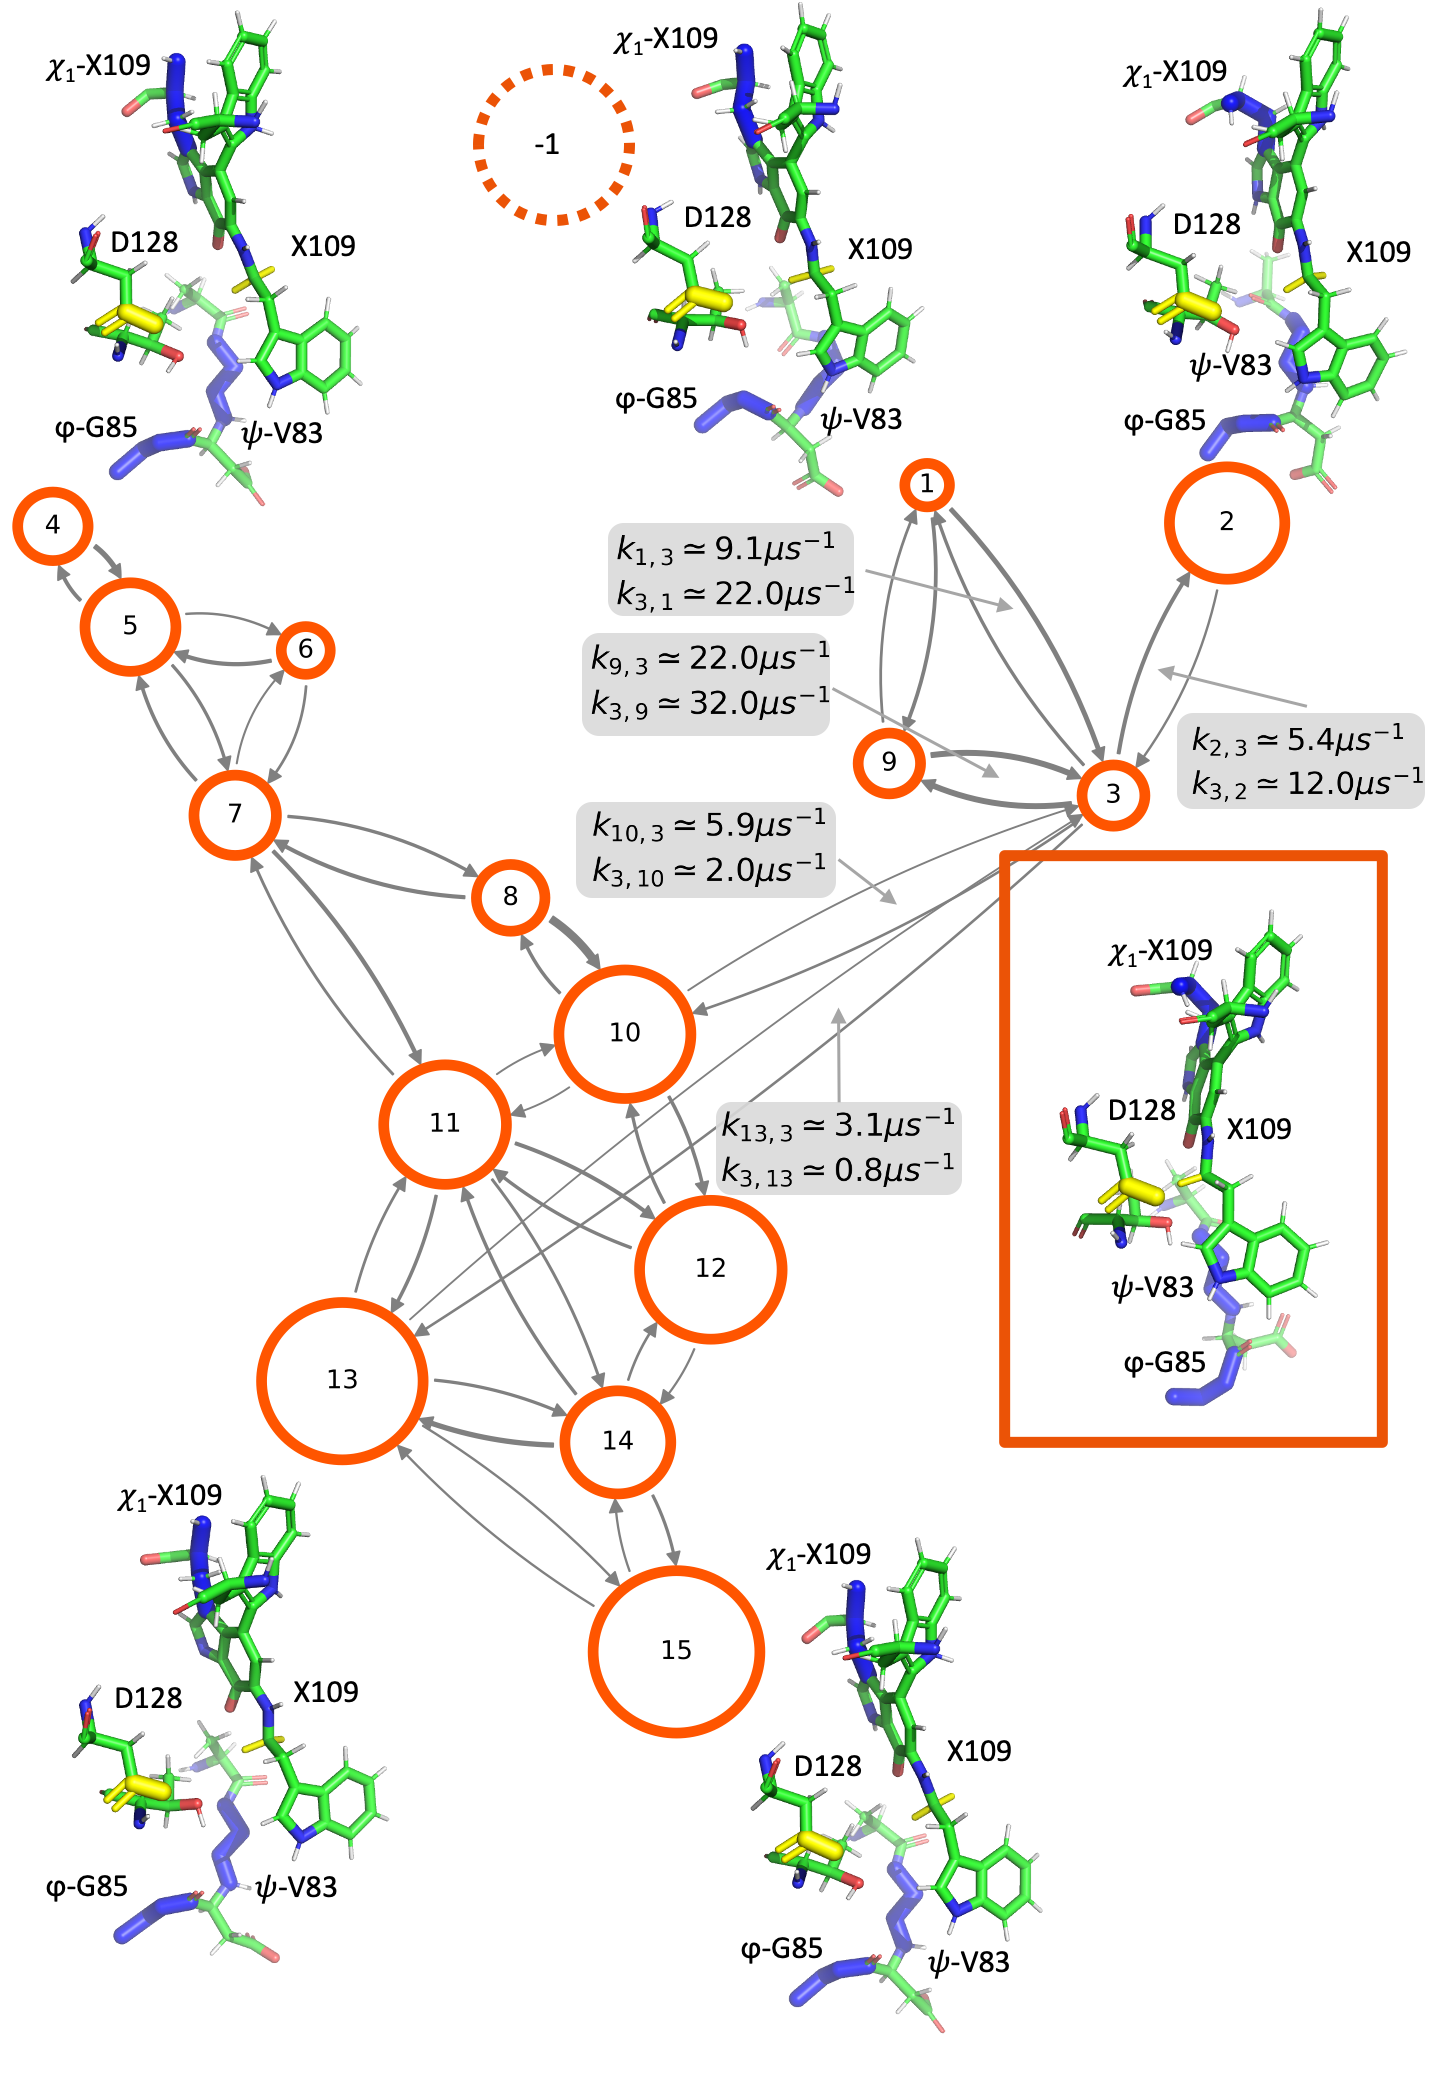
\includegraphics[width=0.9\textwidth]{chapters/aadh/figures/base_case_network_plot.png}
    \label{fig:aadh_base_case_network}
\end{figure}

 The dominant relaxation process (figure \ref{fig:base_case_hmm} panel (a)) transfers population between the relatively populous $h_{2}$ ($\tilde{\pi}_{2} = \SI{10.3}{\percent} [\SIrange[range-phrase=-]{0.1}{73.4}{\percent}]$) to state $h_{15}$ ($\tilde{\pi}_{15}=\SI{23.4}{\percent} [\SIrange[range-phrase=-]{1.6}{91.3}{\percent}$]). From $h_{2}$ to $h_{15}$ the donor-acceptor distance increases from approximately \SI{7.7}{\angstrom} \& \SI{6.1}{\angstrom} to \SI{9.3}{\angstrom} \& \SI{7.5}{\angstrom} to OD1 \& OD2 respectively. However, this process proceeds through the `reactive' state $h_{3}$ with the smallest pair donor-acceptor distances, \SI{5.5}{\angstrom} \& \SI{4.3}{\angstrom}.  
 
 This mechanism is shown in the network plot, figure \ref{fig:aadh_base_case_network}. In this figure the hidden states $i$ and $j$ are only shown connected if the flux between them, $\tilde{\pi}_{i}\tilde{T}_{i,j}$, is greater than \SI{0.01}{\percent}. This is to simplify the picture - the full rate matrix is tabulated in table \ref{tab:base_case_rate_matrix}. The `missing' state $h_{-1}$ is also shown as a disconnected, dashed circle, for reference. Representative structures for a selection of the important states are also shown. In each of these structures bond to OD1, OD2, CI-2, CI-3, are highlighted in yellow and the three most important dihedral angles an highlighted in blue. These angles correspond to the top two largest TICA components in both IC 1 ($\chi_1$-X109 (TTW109) and $\phi$-G85) and IC 2($\chi_1$-X109 and $\psi$-V83). 
 
\begin{figure}
    \centering
    \mycaption[Distribution of important dihedral angles in the base case HMM]{\textsc{Distribution of important dihedral angles in the base case HMM}. The $\chi_{1}$ dihedral angle of TTW 109 for hidden state 2, 3, 13, and 15 are shown in panels (a) - (d); the $\psi$ backbone dihedral of Val83 in panels (e)-(h); and the $\phi$ backbone dihedral of Gly85 in panels (i) - (l). Angles are shown in degrees and have been shifted so that they lie in the range \SIrange{0}{360}{\degree}.}
    \label{fig:aadh_base_case_dihedrals}
    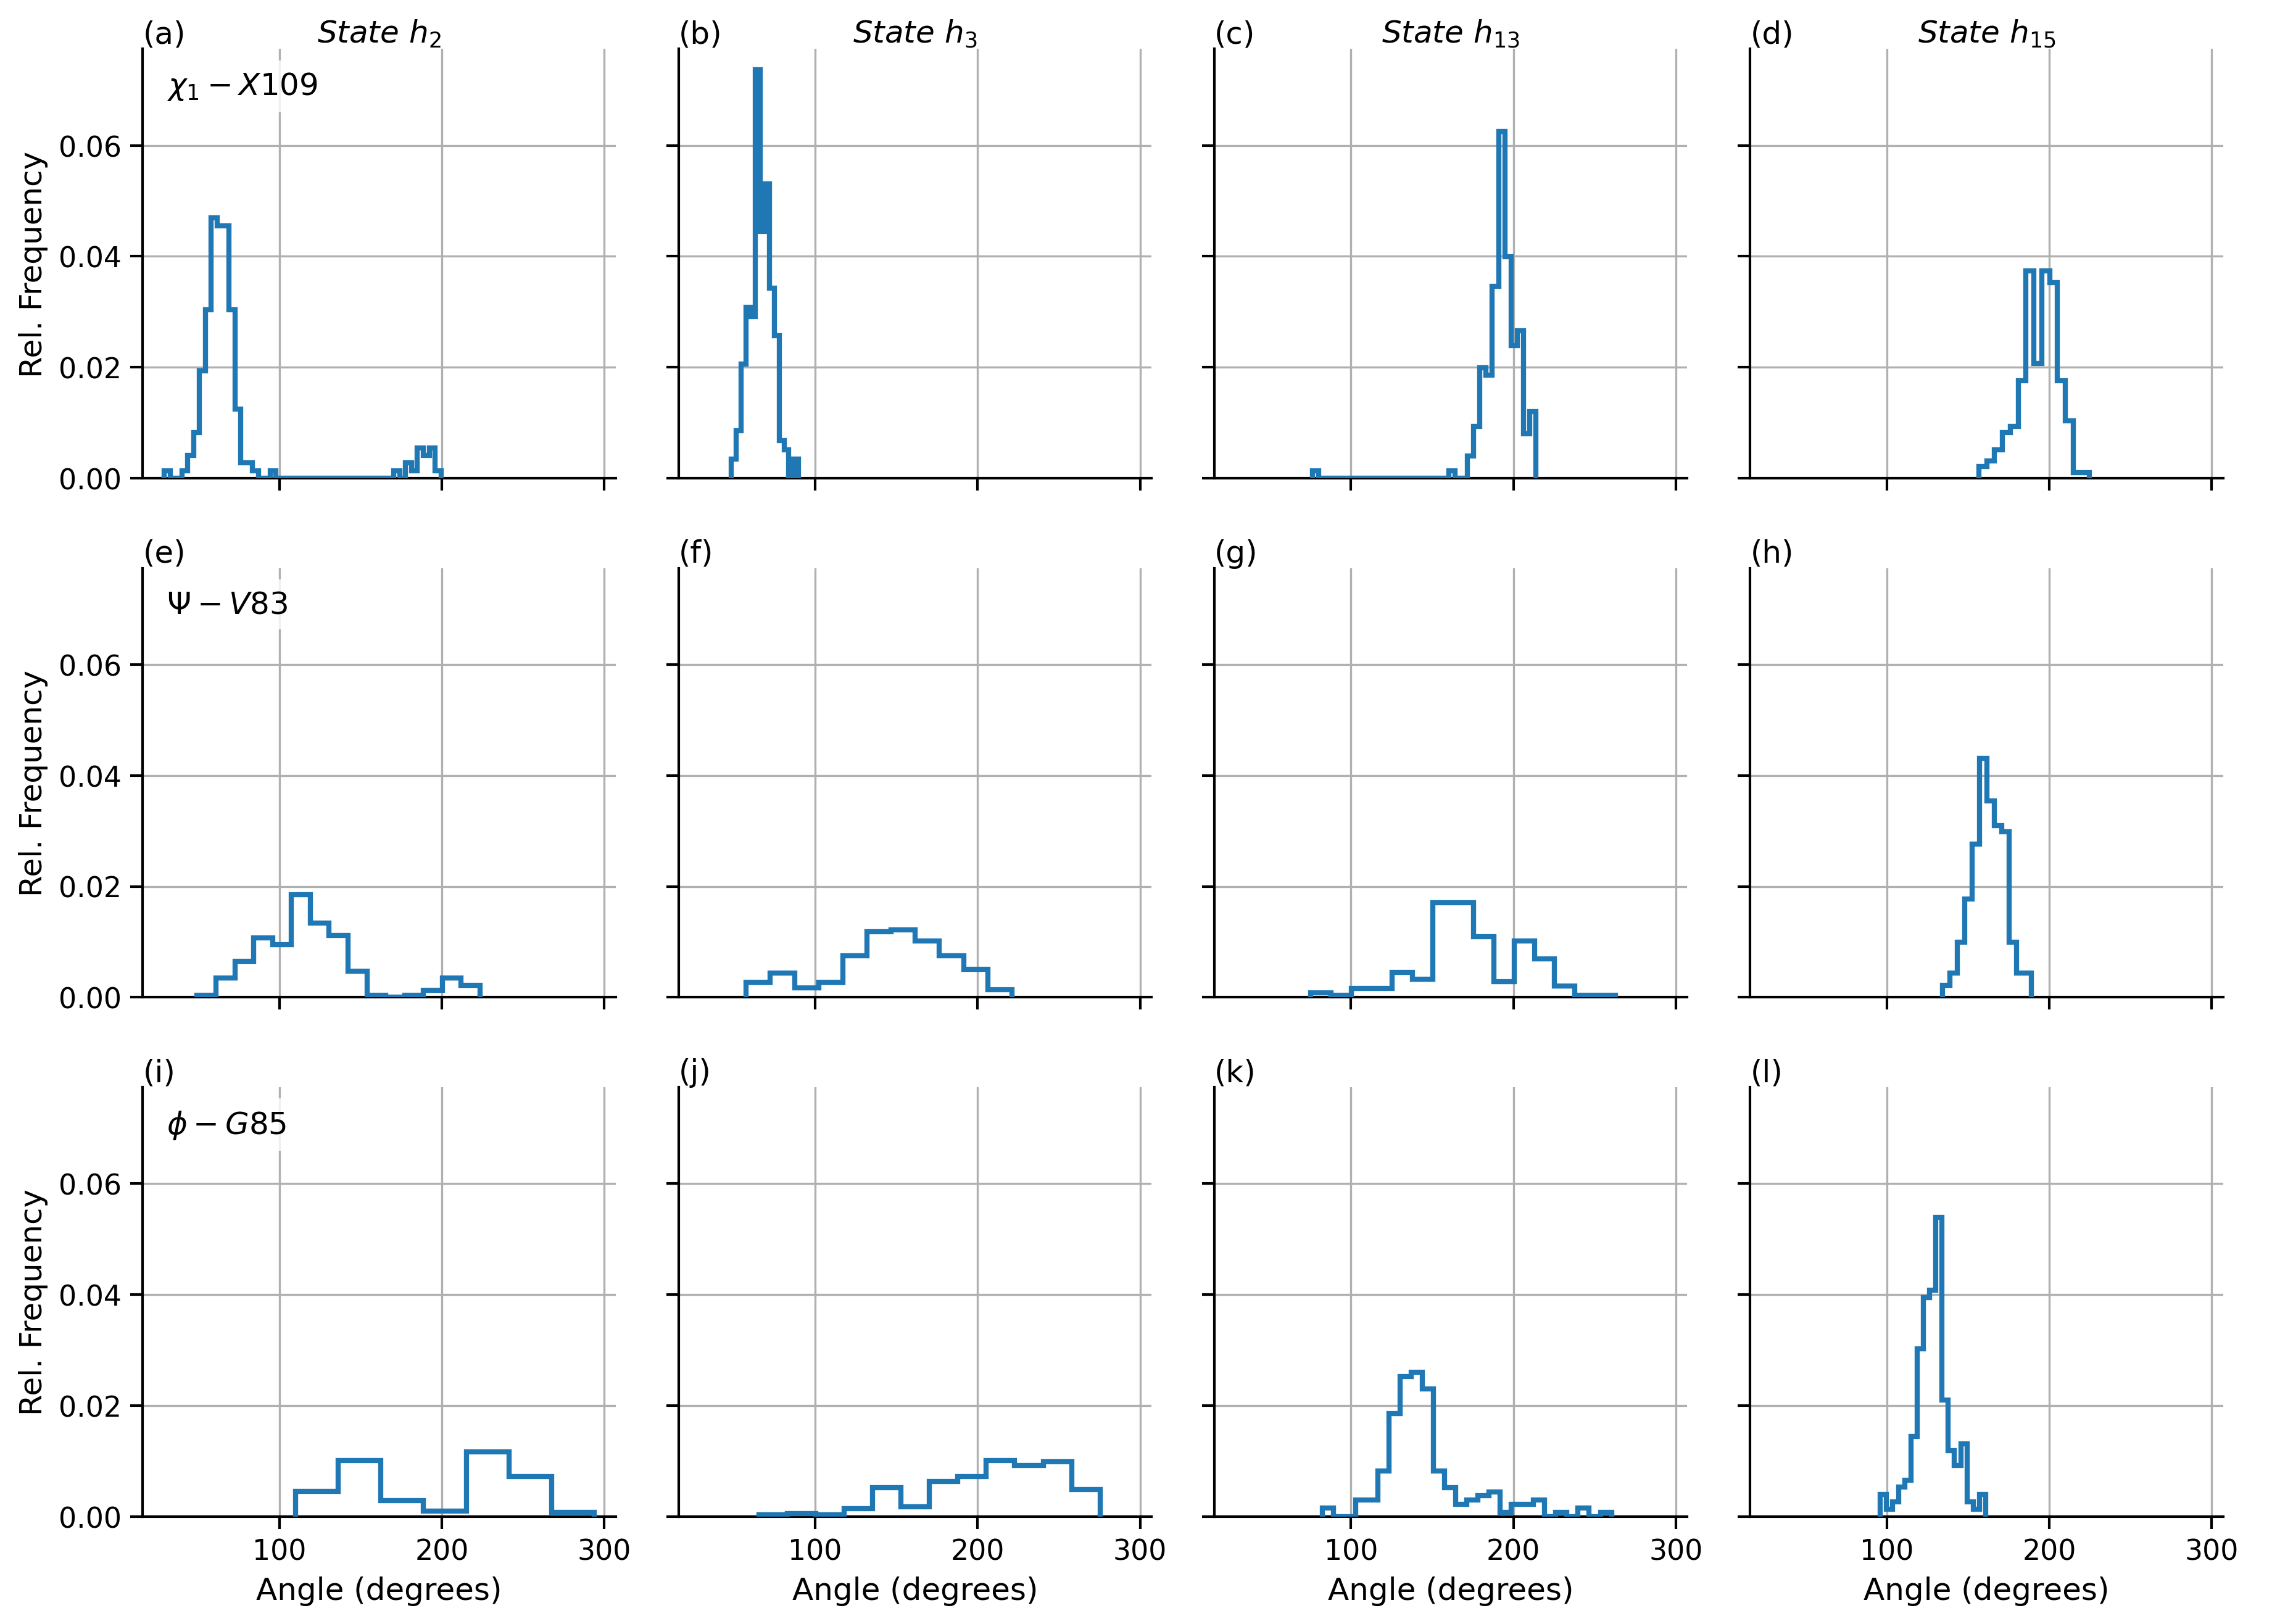
\includegraphics[width=0.8\textwidth]{chapters/aadh/figures/base_case_important_dihedrals.png}
\end{figure}

 In order to understand the slowest  relaxation process in the base case HMM, consider the pathway $h_{2}\rightarrow h_{3} \rightarrow h_{13} \rightarrow h_{15}$. This is the highest flux pathway i.e. the pathway which at each point selects the highest flux connection. The change in the dihedral angles can be seen in the accompanying structures in figure \ref{fig:aadh_base_case_network} and in the distributions plotted in figure \ref{fig:aadh_base_case_dihedrals}.
 The first step, $h_2 \rightarrow h_{3}$, proceed primarily through an increase in both $\phi$-G85 (figure \ref{fig:aadh_base_case_dihedrals} panels (i) and (j)) and $\psi$-V83 (panels (e) and (f)). The second step, $h_{3} \rightarrow h_{13}$, proceeds at a relatively slow rate of  \SI{0.8}{\per\micro\second} [\SIrange[range-phrase=-]{0.0}{4.2}{\per\micro\second}] with a large increase in the $\chi_1$-X109 angle (\ref{fig:aadh_base_case_dihedrals} panels (b) and (c)) from approximately $70^{\circ}$ to $190^{\circ}$. The final step $h_{13}$ to $h_{15}$ proceeds with a decrease in the variance of the $\phi$-G85 and $\psi$-V83 distributions.


The picture arising from the coarse graining sensitivity 2 is very different to the base case, even though the difference in the estimated VAMP-2 score for the MSM was small, base case: $\mu=3.56 \pm 0.18$, sensitivity 2: $\mu=3.44 \pm 0.35$.   First, the hidden states of sensitivity 2 show no large differences in their donor-acceptor lengths which all lie between \SIrange[range-phrase=-]{7.6}{9.1}{\angstrom} to OD1 and \SIrange[range-phrase=-]{5.9}{7.3}{\angstrom} to OD2 as shown in figure \ref{fig:addh_bond_dist_h_state} panels (b) and (d). The stationary distribution is distributed primarily in a single state, $h_{5}$ ($\tilde{\pi}_{5} = \SI{30.12}{\percent}\ [\SIrange{5.27}{68.33}{\percent}]$) and is an order of magnitude more long lived ($\SI{961}{\nano\second}\ [\SIrange[range-phrase=-]{416}{3310}{\nano\second}]$) than either base case $h_{2}$ ($\SI{223}{\nano\second}\ [\SIrange[range-phrase=-]{61.7}{4430}{\nano\second}]$) or $h_{15}$ ($\SI{275}{\nano\second}\ [\SIrange[range-phrase=-]{53.4}{7400}{\nano\second}]$, $h_{15}$). 

Sensitivity 2 state $h_{5}$ is structurally most similar to the base case state $h_{6}$. This was determined by looking at the distributions of RMSDs shown in figure \ref{fig:sens_2_overlap}. The RMSD distribution within each base case hidden state (`BC-BC') and between the base case and sensitivity 2 $h_{5}$ (`BC-S2') were compared to the distribution of RMSD within sensitivity 2 $h_{5}$ (`S2-S2'). For base case state $h_{6}$ distributions were similar and the two states were determined to be the same.  However, base case $h_{6}$ has a much shorter lifetime ($\SI{30.4}{\nano\second}\ [\SIrange[range-phrase=-]{13.2}{110}{\nano\second}]$) and smaller stationary distribution ($\SI{1.6}{\percent}\ [\SIrange[range-phrase=-]{0.1}{5.8}{\nano\second}]$). Despite these differences, the dominant timescale process in both base case and sensitivity two are similar ($\SI{1210}{\nano\second}\ [\SIrange[range-phrase=-]{533}{6590}{\nano\second}]$ for sensitivity 2 and  $\SI{1180}{\nano\second}\ [\SIrange[range-phrase=-]{373}{8180}{\nano\second}]$ for the base case). Despite the small difference in the VAMP-2 scores for the MSMs, the coarse grained models of the base case and sensitivity 2 result in very different models. While this is expected of different features, the similar implied timescales  and the similar VAMP-2 scores suggest that the being able to distinguish between these models will require further analysis and potentially more data collection. 


\section{Conclusions}\label{sec:aadh_conclusions}
AADH is an important system for studying the effects of enzyme dynamics on catalysis due to the large and temperature independent kinetic isotope effect. Previous computational and experimental work determined the mechanism and estimated the free energy barriers using tryptamine as a substrate. The role of dynamics in explaining the temperature independent KIE in AADH is still unresolved. `Active dynamics` on the picosecond timescale have been suggested as facilitating tunneling, while  `passive dynamics', i.e. conformational dynamics, coupled with extensions of transition state theory, have also been suggested as explaining the behaviour of AADH's KIE. 

To investigate the role of conformational dynamics in AADH, \SI{10}{\micro\second} of molecular dynamics simulations of the previously studied Schiff base intermediate were produced. A Markov lag time of $\tau=\SI{2}{\nano\second}$ and the number of dominant eigenvalues, $r=4$, were determined from an exploratory Markov state model. The validity of the simulations was limited however. An error in the preparation of the simulation resulted in a missing an disulphide bond adjacent to the active site in the H chain. The conformations of the H and D chains were radically different although surprisingly the H active site was more similar to the reactive conformations found in previous QM/MM studies. This could be linked to the large conformational change in a loop in chain D which is not observed in chain H, although this was not investigated. In addition, a number of unobserved residues were not modelled and there was significant correlation between each trajectory's initial configuration. 

The response surface of an MSM of the active site, with four hyperparameters ($\chi$, $\tau$, $m$ and $n$), was modelled with a Gaussian process. This highlighted some of the weaknesses of GPs for modelling these types of response surface. First, the conditional structure of the predictor space meant that the RMSD feature was not able to be incorporated into the response surface - a known problem for for GPs in this setting. Second, although standard model selection techniques were used to select the most appropriate GP kernel and input warping, the selected model fit the model with varying success. In particular, the fit of the response surface for the best performing feature, $(\phi, \psi, \chi)$  was less satisfactory than the other features. Third, the hyperparameters which failed to produce a converged MSM were ignored in the response surface modelling. This is ignoring valuable information and in future work this should be incorporated, although it is not clear how this may be achieved effectively. 

However, modelling the hyperparameter response as a GP had a number of practical benefits on top of those mentioned in chapter \ref{chap:msm}. First, it allowed the relevance of hyperparameters to rigorously defined and interpreted for both quasi-continuous (i.e. $\tau, m$ and $n$) as well as categorical (i.e. $\chi$) hyperparameters. This led to the conclusion that the the TICA lag time, $\tau$, is more important in determining the VAMP-2 score than the number of microstates, $n$, in line with the findings from chapter \ref{chap:msm}. This will increase efficiency hyperparameter selection in follow up work on this system, and may generalize to other systems.  Second, the relevance of the hyperparameters was able to guide efficient visualisation of the five-dimensional response surface, enabling suitable sensitivity analysis to be performed. Making use of the relevance in this way will be useful for not only MSMs but for understanding and optimising other complex statistical and machine learning models. 

Bayesian optimisation was used to optimise the MSM response, although this did not affect the final set of hyperparameters appreciably. Despite this, the optimisation step was important to confirm the convergence of the MSM response surface. By seeding the optimisation algorithm with fewer observations, BO was able to find the maximum of the response surface with a smaller overall number of MSM evaluations. Although not conclusive, this work will hopefully encourage further research in this area to further reduce the amount of computational resources necessary for optimising MSMs. 

The ICL was used to select the number of hidden states in maximum likelihood HMMs used to coarse grain the base case and sensitivity analysis MSMs. The selected HMMs were re-estimated using a Bayesian analysis in order to quantify the uncertainty in the model observables. This method is attractive because maximum likelihood models are relatively quick to estimate and the ICL requires negligible extra calculations. The more laborious Bayesian fitting procedure can then be reserved for models with higher probability of being useful. This meant that a large number of models could be quickly assessed for goodness-of-fit. However, this approach was not satisfactory for a number of reasons. First, the difference in the way the maximum likelihood and Bayesian HMMs are estimated means that the number of reversibly connected hidden states differed between the Maximum likelihood and Bayesian approaches. This renders the interpretation of the ICL (as the model with the greatest evidence for observed and hidden state structure) meaningless. Second, in the case of sensitivity 1 and 3 the selected Bayesian models could not be estimated at all. Additionally, the base case and sensitivity 2 models could not be validated via a Chapman-Kolmogorov test. This may be the result of the large number of hidden states selected by the ICL or due to the effectively small amount of data. In order to resolve this issue and to better understand the potential for the ICL in model selection for biomolecular HMMs more independent simulation data is needed. 

Despite the limitations of the base case model, the picture arising shows the active site has a ensemble of short lived (\SIrange{20}{300}{\nano\second}) metastable states, with one state with a significantly shorter donor-acceptor distance than the others (approximately $\SI{4}{\angstrom})$. This state is a flux bottle neck state between two long lived states which interconvert on a timescale of approximately $\SI{1.2}{\micro\second}$, primarily as the result of a rotation in the $\chi_1$ dihedral angle on the TTW residue. The reason why this process proceeds through bottle neck state has not been elucidated. Sensitivity 2 is a model with a similar, but smaller, value of VAMP-2 score for the corresponding MSM, but the picture arising does not back up that from the base case model. This either sheds doubt on the robustness of the conclusions from base case model, or on the ability of VAMP-2 score to differentiate between models with the amount of data collected here. A program of future work to address these issues and extend this work is presented in chapter \ref{chap:conclusions}.  









% \begin{figure}
%     \centering
%     \mycaption{The ratio of implied timescales (panels (a), (c), (e), (g)) and eigenvalues (panels (b), (d), (f), (h)) for base case and three sensitivity cases respectively. The values were estimated from a  corresponding  Bayesian MSM using 1000 draws from the posterior. The error bars are the \SI{95}{\percent} credible intervals}
%     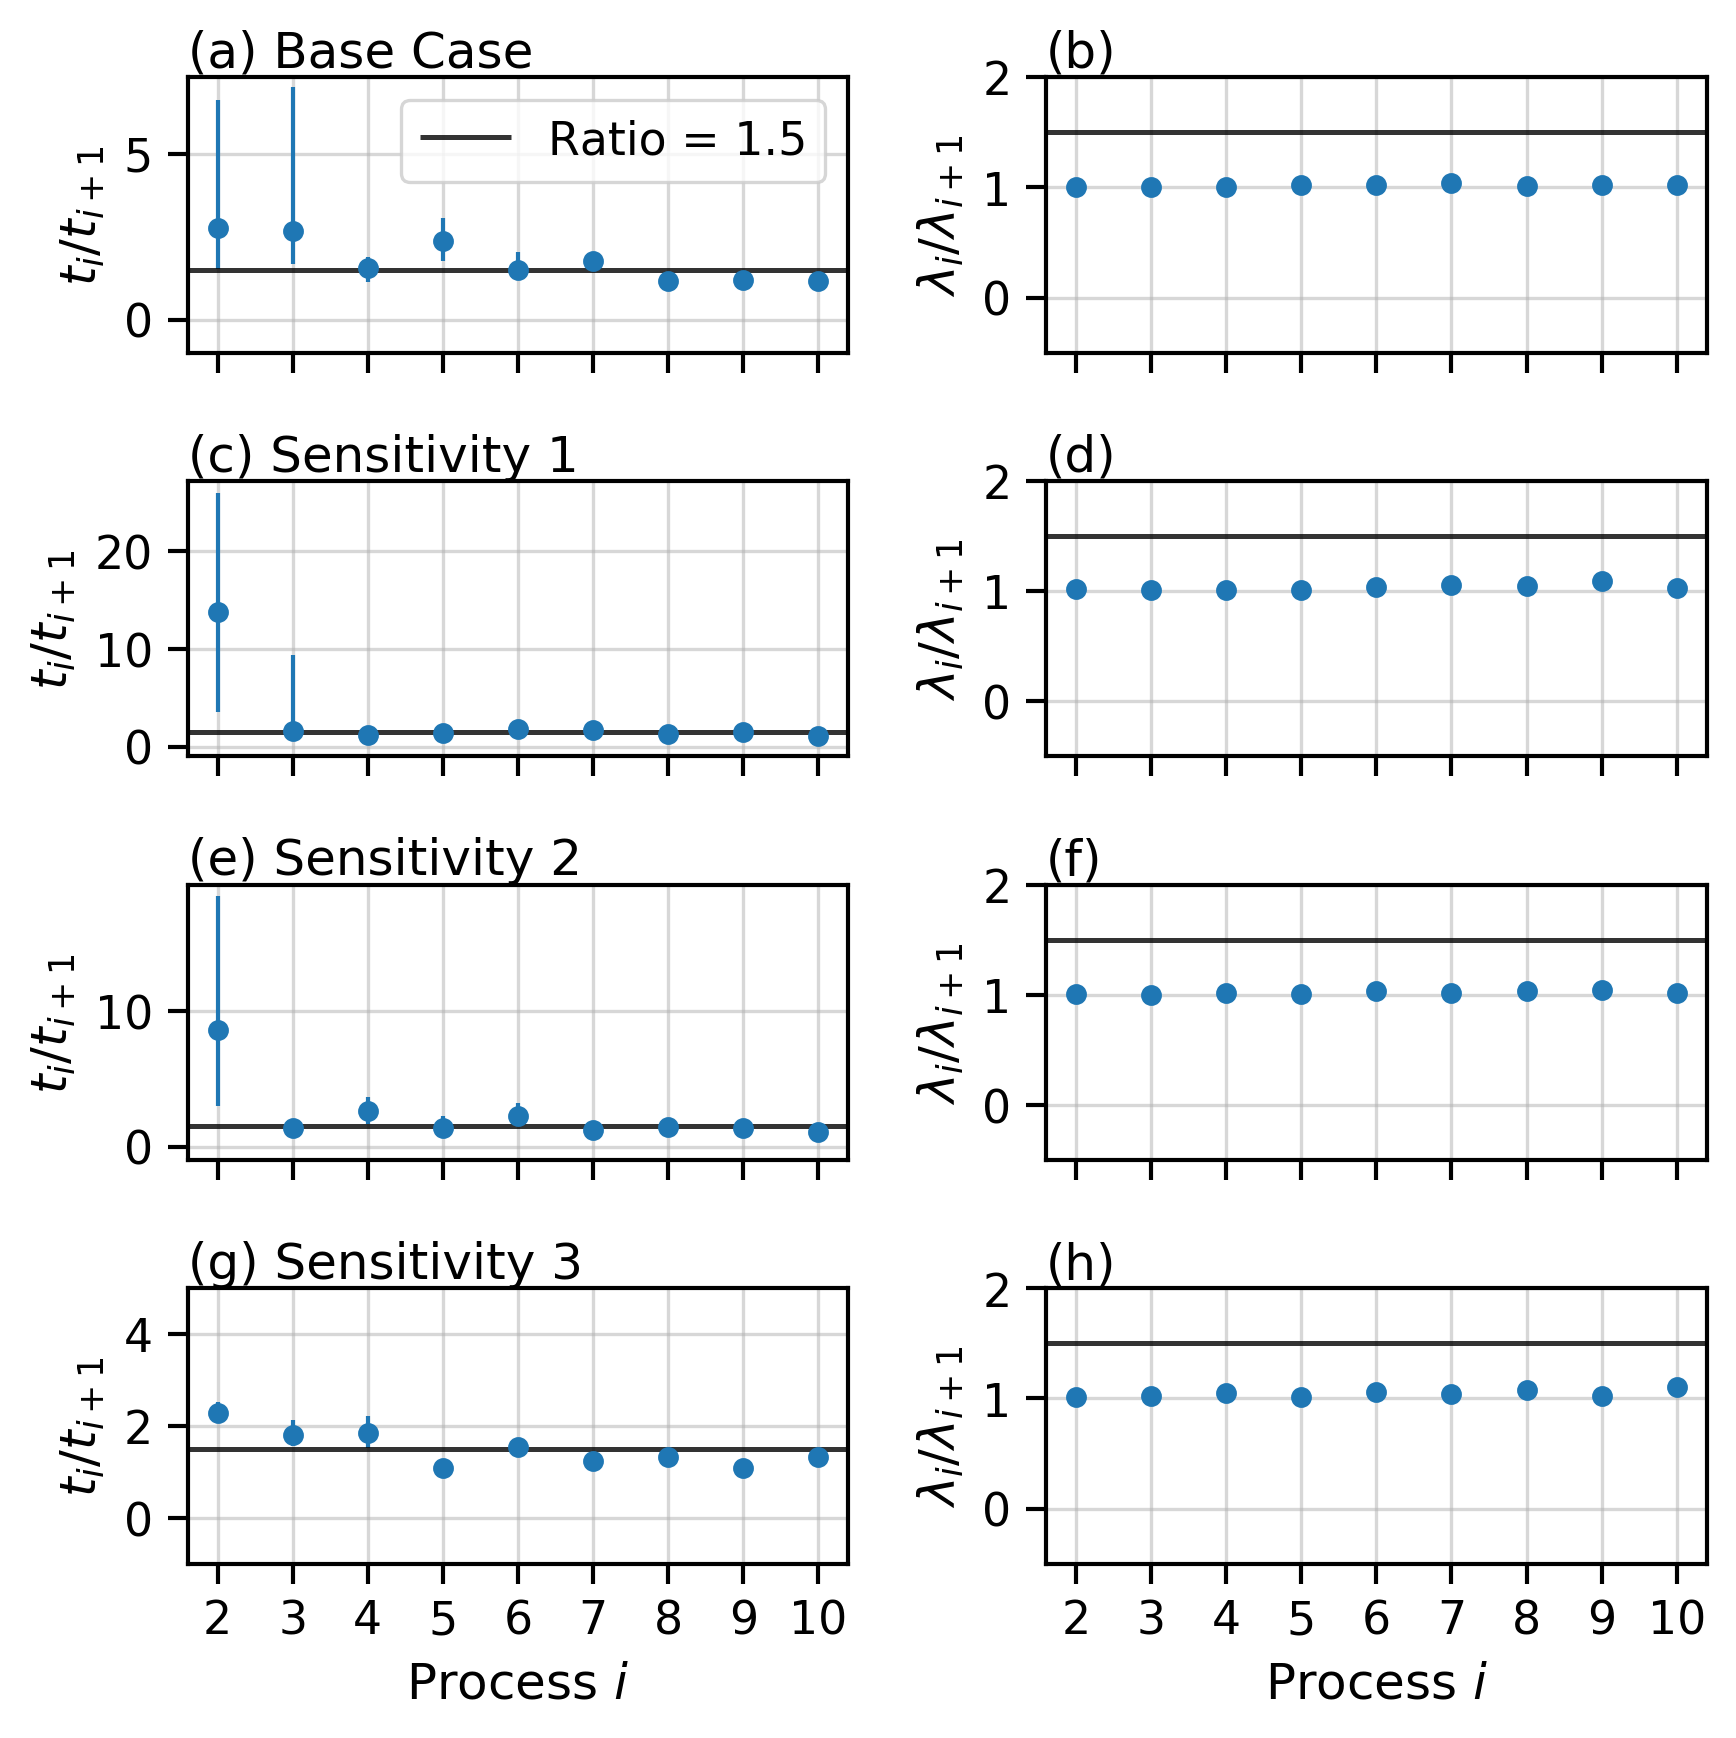
\includegraphics[width=0.8\textwidth]{chapters/aadh/figures/aadh_its_evs.png}
%     \label{fig:aadh_its_evs_results}
% \end{figure}
% \begin{table}
%     \centering
%     \mycaption{Mean implied timescales and $\SI{95}{\percent}$ credible intervals (in nanoseconds) of the relaxation processes 2 - 10 for the base case and three sensitivities.}

%     \begin{tabular}{|l|l|l|l|l|}
%     \hline
%      &             Base Case &            Sensitivity 1 &         Sensitivity 2 &      Sensitivity 3 \\
%     Process &                       &                          &                       &                    \\
%     \hline\hline
%     2       &  2,117 (1,033, 5,214) &  25,843 (15,913, 41,797) &  2,694 (1,352, 4,606) &   152 ( 138,  169) \\
%     3       &     988 ( 479, 1,669) &     2,748 (1,510, 5,458) &      408 ( 312,  716) &    67 (  64,   71) \\
%     4       &      231 ( 195,  276) &      1,101 ( 553, 2,256) &      304 ( 234,  397) &    36 (  31,   43) \\
%     5       &      138 ( 129,  149) &         563 ( 497,  668) &      155 (  79,  252) &    20 (  19,   23) \\
%     6       &       54 (  43,   73) &         482 ( 412,  566) &       80 (  52,  115) &    18 (  17,   20) \\
%     7       &       38 (  33,   43) &         418 ( 327,  463) &       30 (  26,   38) &    12 (  11,   13) \\
%     8       &       23 (  21,   26) &         228 ( 205,  249) &       25 (  22,   29) &     9 (   8,   10) \\
%     9       &       21 (  18,   23) &         137 ( 115,  163) &       17 (  15,   18) &     7 (   7,    8) \\
%     10      &       16 (  15,   19) &         105 (  99,  110) &       12 (  11,   15) &     7 (   6,    7) \\
%     \hline
%     \end{tabular}
%     \label{tab:sens_ts}
% \end{table}